\documentclass{article}


% if you need to pass options to natbib, use, e.g.:
%     \PassOptionsToPackage{numbers, compress}{natbib}
% before loading neurips_2022
% \PassOptionsToPackage{sort,numbers,compress}{natbib}
% \PassOptionsToPackage{sort,authoryear,compress}{natbib}

% ready for submission
% \usepackage{neurips_2022}
\usepackage[utf8]{inputenc} % allow utf-8 input
\usepackage[T1]{fontenc}    % use 8-bit T1 fonts
\usepackage[normalem]{ulem}
\usepackage[margin=1in]{geometry}
\usepackage[numbers,sort]{natbib}
\usepackage{amsmath}
\usepackage{amsthm, amssymb, thmtools, thm-restate}
\usepackage{bbm}
\usepackage{minitoc}
\usepackage{subfigure}
\usepackage{algorithm}
\usepackage{algorithmicx}
\usepackage{algpseudocode}
\usepackage{nicefrac}
\usepackage{booktabs}       % professional-quality tables
\usepackage{amsfonts}       % blackboard math symbols
\usepackage{nicefrac}       % compact symbols for 1/2, etc.
\usepackage{microtype}      % microtypography
\usepackage{xcolor}         % colors
\usepackage{url}            % simple URL typesetting
\usepackage{hyperref}
\usepackage{enumitem}
\usepackage[capitalise]{cleveref}
\usepackage{authblk}
\bibliographystyle{unsrtnat}

\newcommand{\red}[1]{\textcolor{red}{#1}}
\newcommand{\blue}[1]{\textcolor{blue}{#1}}
\def\*#1{\boldsymbol{#1}}


\newtheorem{theorem}{Theorem}
\newtheorem{lemma}{Lemma}
\newtheorem{proposition}{Proposition}
\newtheorem{corollary}{Corollary}
\newtheorem{observation}{Observation}
\newtheorem{definition}{Definition}
\newtheorem{claim}{Claim}
\newtheorem{fact}{Fact}
\newtheorem{assumption}{Assumption}
\crefname{assumption}{Assumption}{Assumptions}
\newtheorem{example}{Example}
\crefname{example}{Example}{Examples}

\declaretheorem[name=Theorem]{thm}
\crefname{thm}{Theorem}{Theorems}
\declaretheorem[name=Lemma]{lem}
\crefname{lem}{Lemma}{Lemmas}
\declaretheorem[name=Proposition]{prop}
\crefname{prop}{Proposition}{Propositions}
\declaretheorem[name=Corollary]{cor}
\crefname{cor}{Corollary}{Corollaries}

\allowdisplaybreaks

\hypersetup{
    colorlinks,
    linkcolor={blue!50!black},
    citecolor={blue!50!black},
    urlcolor={blue!80!black}
}

\title{Maximizing Communication Efficiency for Large-scale Training via 0/1 Adam}

\newcommand{\myparagraph}[1]{\textbf{#1}\hspace{0.5em}}
\newcommand{\myalgo}{\textbf{0/1 Adam}}
% Todonotes is useful during development; simply uncomment the next line
%    and comment out the line below the next line to turn off comments
%\usepackage[disable,textsize=tiny]{todonotes}
\usepackage[textsize=tiny]{todonotes}

\newcommand{\yucheng}[1]{\textcolor{red}{Yucheng: #1}}
\allowdisplaybreaks

\author[2]{Yucheng Lu\thanks{Corresponds to: yl2967@cornell.edu.}}
\author[1]{Conglong Li}
\author[1]{Minjia Zhang}
\author[2]{Christopher De Sa}
\author[1]{Yuxiong He}
\affil[1]{Microsoft}
\affil[2]{Department of Computer Science, Cornell\ University}
\date{}

\newcommand {\minjia}[1]{{\color{orange}\sf{[Minjia: #1]}}}

\begin{document}

\maketitle

\begin{abstract}
As a popular paradigm for juggling data privacy and collaborative training, federated learning~(FL) is flourishing to distributively process the large scale of heterogeneous datasets on edged clients. Due to bandwidth limitations and security considerations, it ingeniously splits the original problem into multiple subproblems to be solved in parallel, which empowers \textit{primal dual} solutions to great application values in FL. In this paper, we review the recent development of classical \textit{federated primal dual} methods and point out a serious common defect of such methods in non-convex scenarios, which we say is a ``dual drift'' caused by dual hysteresis of those longstanding inactive clients under partial participation training. To further address this problem, we propose a novel \textit{\textbf{A}ligned \textbf{Fed}erated \textbf{P}rimal \textbf{D}ual}~(\textit{\textbf{A-FedPD}}) method, which constructs virtual dual updates to align global consensus and local dual variables for those protracted unparticipated local clients. Meanwhile, we provide a comprehensive analysis of the optimization and generalization efficiency for the \textit{A-FedPD} method on smooth non-convex objectives, which confirms its high efficiency and practicality. Extensive experiments are conducted on several classical FL setups to validate the effectiveness of our proposed method. 
\end{abstract}
%%%%%%%%%%%%%%%%%%%%%%%%%%%%%%%%%%%%%%%%%%%%%%%%%%
\section{Introduction}
\label{main:sec:introduction}
%%%%%%%%%%%%%%%%%%%%%%%%%%%%%%%%%%%%%%%%%%%%%%%%%%

\glsresetall

% \ljh{Just a draft. need polishing and proofreading}
A \gls{np}~\citep{garnelo2018conditional,garnelo2018neural} meta-learns a stochastic process describing the relationship between inputs and outputs in a given data stream, where each task in the data stream consists of a meta-training set of input-output pairs and also a meta-validation set. The \gls{np} then defines an implicit stochastic process whose functional form is determined by a neural network taking the meta-training set as an input, and the parameters of the neural network are optimized to maximize the predictive likelihood for the meta-validation set. This approach is philosophically different from the traditional learning pipeline where one would first elicit a stochastic process from the known class of models (e.g., \glspl{gp}) and hope that it describes the data well. An ideal \gls{np} would assume minimal inductive biases and learn as much as possible from the data. In this regard, \glspl{np} can be framed as a ``data-driven'' way of choosing proper stochastic processes.

 An important design choice for a \gls{np} model is how to capture the uncertainty in the random functions drawn from stochastic processes. When mapping the meta-training set into a function, one might employ a deterministic mapping as in \citet{garnelo2018conditional}. However, it is more natural to assume that there may be multiple plausible functions that might have generated the given data, and thus encode the functional (epistemic) uncertainty as a part of the \gls{np} model. \citet{garnelo2018neural} later proposed to map the meta-training set into a fixed dimensional \emph{global latent variable} with a Gaussian posterior approximation. While this improves upon the vanilla model without such a latent variable~\citep{le2018empirical}, expressing the functional uncertainty only through the Gaussian approximated latent variable has been reported to be a bottleneck~\citep{louizos2019functional}. To this end, \citet{lee2020bootstrapping} and \citet{lee2022neural} propose to apply bootstrap to the meta-training set to use the uncertainty arising from the population distribution as a source for the functional uncertainty.

In this paper, we take a rather different approach to define the functional uncertainty for \glspl{np}. Specifically, we utilize the martingale posterior distribution~\citep{fong2021martingale}, a recently developed alternative to conventional Bayesian inference. In the martingale posterior, instead of eliciting a likelihood-prior pair and inferring the Bayesian posterior, we elicit a joint predictive distribution on future data given observed data. Under suitable conditions on such a predictive distribution, it can be shown that the uncertainty due to the generated future data indeed corresponds to the uncertainty of the Bayesian posterior. Following this, we endow a \gls{np} with a joint predictive distribution defined through neural networks and derive the functional uncertainty as the uncertainty arising when mapping the randomly generated future data to the functions. Compared to the previous approaches of either explicitly positing a finite-dimensional variable encoding the functional uncertainty or deriving it from a population distribution, our method makes minimal assumptions about the predictive distribution and gives more freedom to the model to choose the proper form of uncertainty solely from the data. Due to the theory of martingale posteriors, our model guarantees the existence of the martingale posterior corresponding to the valid Bayesian posterior of an implicitly defined parameter. 
% \ed{Does the following make sense: }
Furthermore, working in the space of future observations allows us to incorporate the latent functional uncertainty path with deterministic path in a more natural manner.
% \ljh{It would be good to have more concrete motivation to prefer the martingale posteriors over conventional Bayesian inference; what would be an advantage of doing that, aside from the fact that we don't need to choose likelihood and prior?} \ed{I'll have a think about this, and will also do some proofreading. Because of the time difference and my job hours, timing might be a bit tricky tomorrow. When would be the best time for me to proofread?}

We name our extension of \glspl{np} with the joint predictive generative models as the \gls{mpnp}. Throughout the paper, we propose an efficient neural network architecture for the generative model that is easy to implement, flexible, and yet guarantees the existence of the martingale posterior. We also propose a training scheme to stably learn the parameters of \glspl{mpnp}. Using various synthetic and real-world regression tasks, we demonstrate that \gls{mpnp} significantly outperforms the previous \gls{np} variants in terms of predictive performance.





% \gls{npf}~\citep{garnelo2018conditional, garnelo2018neural} is a class of parametric models which defines stochastic processes over given data using neural networks.
% Unlike classical stochastic processes (e.g. \glspl{gp}), \gls{npf} learns to fit a proper stochastic processes from data under meta-learning framework.
% The deterministic version of \gls{npf}, \glspl{cnp}~\citep{garnelo2018conditional} deterministically map each dataset to a certain stochastic process which does not consider functional uncertainty.
% In order to compensate for this problem, \glspl{np}~\citep{garnelo2018neural} introduce a global latent variable which captures functional uncertainty.
% \citet{le2018empirical} empirically shows that considering functional uncertainty in \glspl{np} improves the diversity in function realizations and the predictive performance for data.

% Although \glspl{np} tries to capture functional uncertainty, there is some limitations for \glspl{np} to well capture uncertainty with a Gaussian latent variable.
% To overcome this problem, there are some prior works which applying advanced functional uncertainty modeling strategies~\citep{lee2020bootstrapping}\citep{lee2022neural} instead of a global latent variable.
% \gls{bnp}~\citep{lee2020bootstrapping} employs the residual bootstrapping strategy to make more robust uncertainty estimation even for the data-model mismatch situation. 
% However, \gls{bnp} requires a high computational cost compared to \gls{np} due to it's residual bootstrapping strategy.
% \gls{neubnp}~\citep{lee2022neural} employs the recent computationally efficient bootstrapping of the neural network called Neural Bootstrapper~\citep{shin2021neural}.
% However, \gls{neubnp} multiplies Dirichlet distributed random bootstrap weights to features of context dataset which disturbs model to well recovers the given dataset.

% This paper presents a novel extension of \gls{npf} which introduces functional uncertainty by changing posterior uncertainty on function parameters as predictive uncertainty on the unseen data conditional on the observed data...

\section{Related Work}
\label{sec:related work}
\textbf{Communication-efficient training.}
There has been various lines of research focusing on improving communication efficiency in large-scale training, such as using asynchrony \citep{niu2011hogwild,lian2015asynchronous,xie2020zeno++}, decentralization \citep{lian2017can,lu2021optimal}, gradient quantization \citep{alistarh2017qsgd,wen2017terngrad}, gradient sparsification \citep{wangni2017gradient,wang2018atomo}, local steps \citep{stich2018local,lin2018don}, etc. 
In this paper we study the aggressive 1-bit compression, which was first introduced in \citep{seide20141} to speed up speech model training, where an algorithm called 1-bit SGD is proposed. After that, \citet{wen2017terngrad} proposes adding 0 as an additional numerical level and \citet{liu2018signsgd} discusses the use of zero-th order oracle in 1-bit SGD. \citet{chen2019distributed,balles2018dissecting,xu2019signprox} study the correlation and combination between 1-bit SGD and other techniques. Convergence analysis on 1-bit SGD is given in \citep{bernstein2018signsgd,karimireddy2019error,safaryan2021stochastic}. 
\citet{bernstein2018signsgd2,sohn2019election,le2020distributed,lyu2021dp} investigate the robustness of 1-bit SGD.
Among all the variants of 1-bit communication, the design with error feedback mechanism has shown to work best both empirically \citep{seide20141} and theoretically \citep{karimireddy2019error}.
Other lines of research applies 1-bit communication to various scenarios such as federated learning \citep{jin2020stochastic,yue2021federated}, decentralized learning \citep{lu2020moniqua,koloskova2019decentralized}, meta learning \citep{fan2021sign}, etc. Perhaps the closest works to this paper are \citep{tang20211,li20211}, which propose using two-stage training to enable 1-bit Adam and 1-bit Lamb, respectively. Different from those two work, 0/1 Adam addresses non-linearity challenges in adaptive optimizers by considering both extreme quantization and local steps. Furthermore, we also study how to apply extreme communication compression on GPT-style models, which to the best our knowledge is still under-explored.  

\textbf{Adaptive learning rate optimizers.}
One of the most popular adaptive optimizers is Adam, which was first introduced in \citep{kingma2014adam}. It uses both first and second moment information of stochastic gradient to perform optimizer steps and has shown significant benefits on training deep learning models. \citet{reddi2019convergence} spots the issue of Adam convergence and provides a variant called AMSGrad while \citet{zaheer2018adaptive} argues the Adam only converges with large batch sizes.
Multiple lines of theoretical study on Adam are given in \citep{fang2019convergence,alacaoglu2020new,defossez2020simple}.
Additionally,
\citet{chen2018convergence,zhou2018convergence,lu2020mixml,danilova2020recent,zou2019sufficient} provide more general analysis on Adam-type optimizers.
Subsequently, other variants of Adam are proposed in \citep{luo2019adaptive,chen2019zo,huang2018nostalgic,wang2019sadam, zhou2018adashift, zhuang2021momentum,zhuang2020adabelief}. 
Unlike these methods, which focus on improving the convergence of generic optimizations for DNN models, our work studies how to maximize the communication efficiency of Adam in large-scale distributed training settings. 

% the communication efficiency of Adam in data-center model training.
% We emphasize there is a major distinction between these previous works and {\myalgo}, as they 
% investigates how to improve Adam statistically while {\myalgo} studies the communication efficiency of Adam in data-center model training.
\section{A Closer Look at Non-linearity in Adam}
\label{sec:motivation}
\begin{figure*}[t!]
  \centering
  \subfigure[$\|\*v_t-\*v_{t-1}\|$]{
  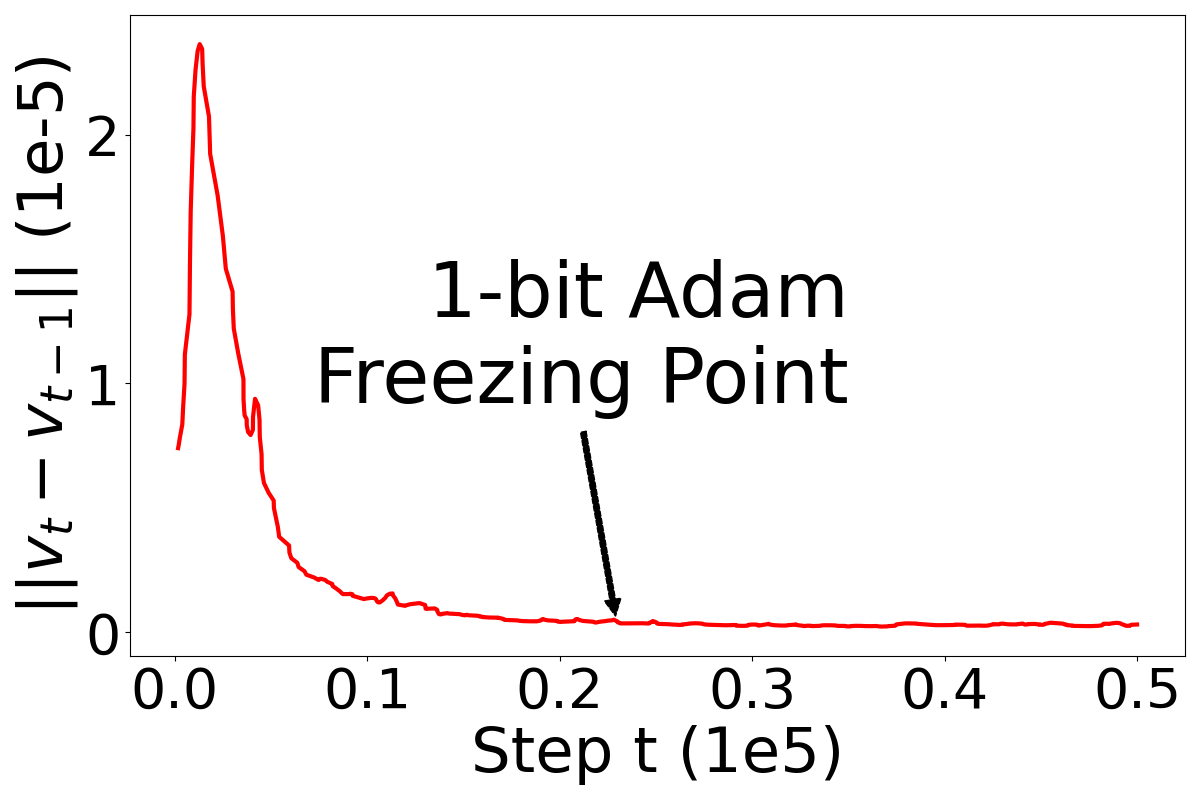
\includegraphics[width=0.23\textwidth]{./sections/figure/v_diff.png}\label{fig:profile_bert_large:var_diff_time}}
  \subfigure[$\|\*v_t^{(0)}-\*v_t\|$]{
  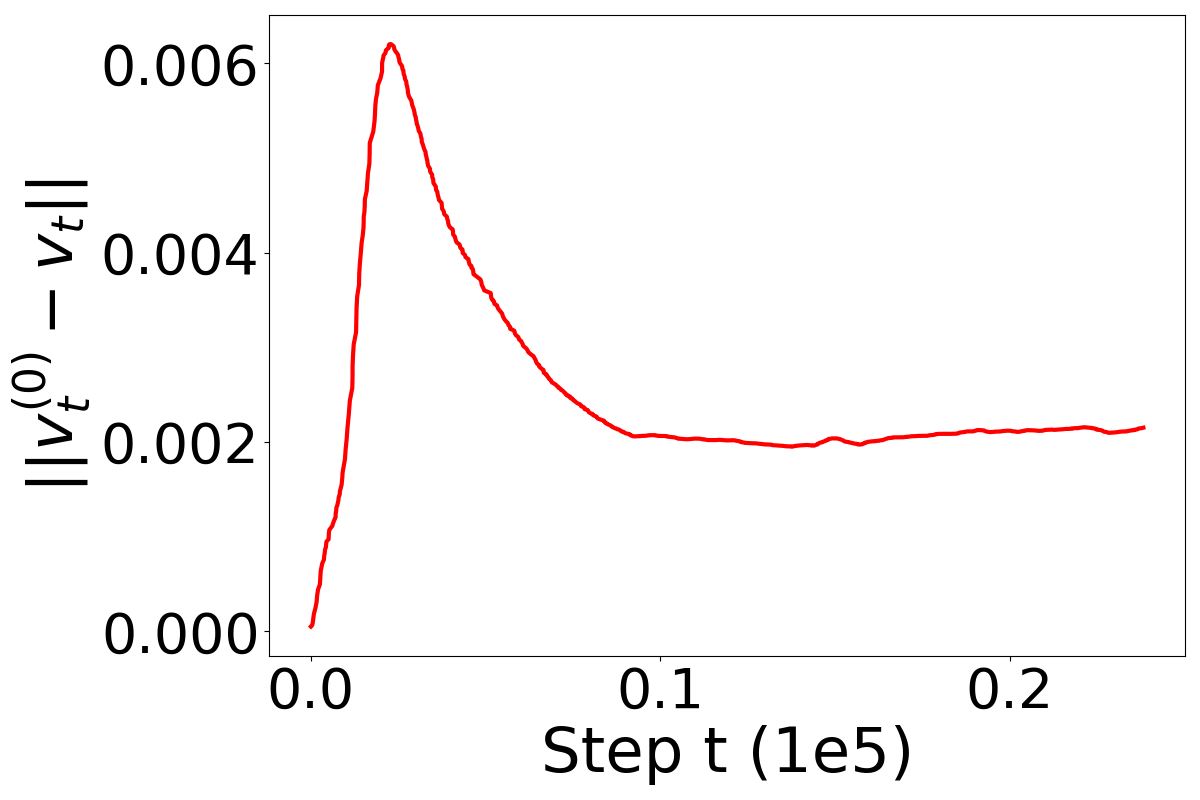
\includegraphics[width=0.23\textwidth]{./sections/figure/v_diff_local.png}\label{fig:profile_bert_large:var_diff_local}}
  \subfigure[$\|\*m_t-\*m_{t-1}\|$]{
  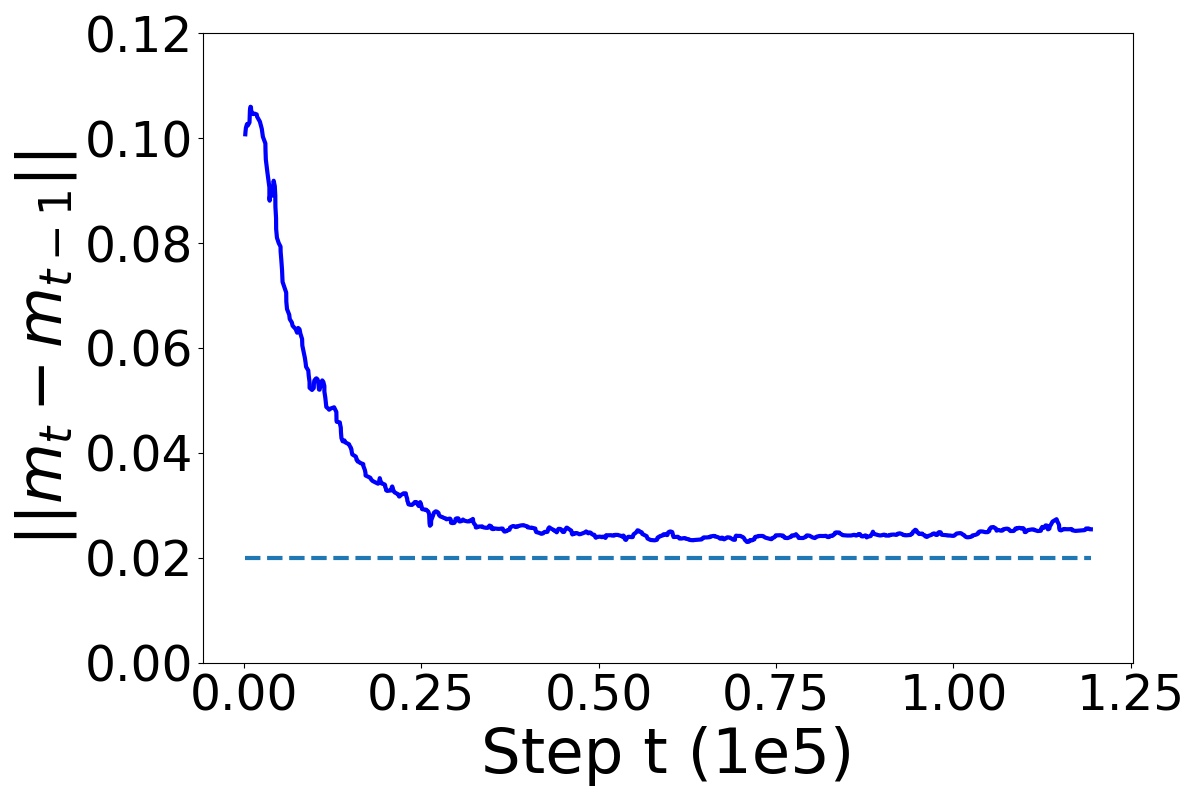
\includegraphics[width=0.23\textwidth]{./sections/figure/m_diff.png}\label{fig:profile_bert_large:mom_diff_time}}
  \subfigure[$\|\*m_t^{(0)}-\*m_t\|$]{
  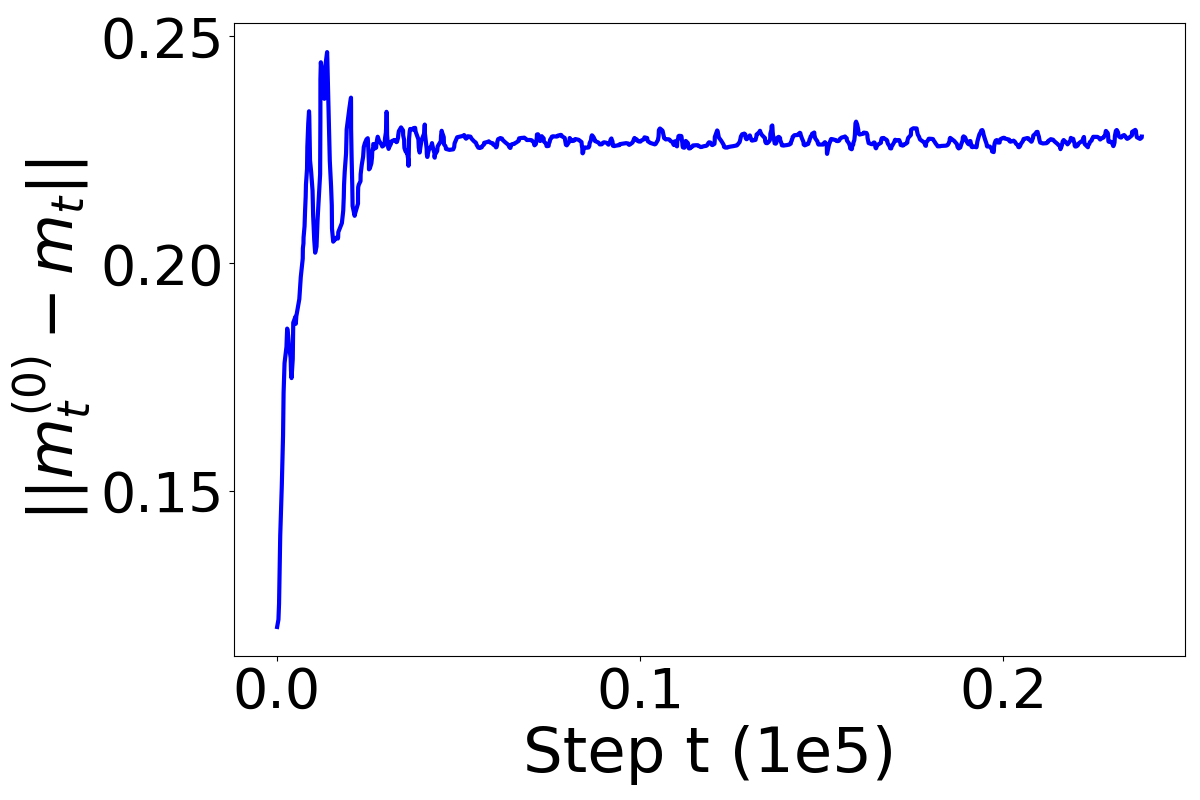
\includegraphics[width=0.23\textwidth]{./sections/figure/m_diff_local.png}\label{fig:profile_bert_large:mom_diff_local}}
  \caption{Momentum and variance Profiling for BERT-Large sequence 128 pretraining with original Adam using 64 GPUs. For variance, we profile two types of metrics: the first is the difference between local and global variance: $\|\*v_t^{(0)}-\*v_t\|$, where $\*v_t^{(0)}$ and $\*v_t$ denotes the variance term computed via local gradient on worker-0 and the gradient from full-precision AllReduce, respectively. We also profile the variance difference in adjacent step $\|\*v_t-\*v_{t-1}\|$. Similarly, we profile the same two metrics for the momentum.}
  \label{fig:profile_bert_large}
\end{figure*}

In this section, we provide a more formal description on the problem setting and illustrate the limitations from the original Adam and the state-of-the-art 1-bit Adam \citep{tang20211}.

\textbf{Problem Formulation.}
In this paper, we consider the following optimization problem:
\begin{align}
    \min_{\*x\in\mathbb{R}^d}f(\*x) = \mathbb{E}_{\zeta\sim\mathcal{D}}f(\*x;\zeta).
\end{align}
where $\*x$ denotes the $d$-dimensional model. $\mathcal{D}$ denotes the training set and $f(\*x;\zeta)$ is the loss incurred over sample $\zeta$ given model parameters $\*x$.
The structure of the problem naturally captures many of the model training problems.

\textbf{The non-linearity in Adam.}
At step $t\geq 0$, denote $\*x_t$ and $\*g_t$ as the model parameters and stochastic gradient computed at step $t$, respectively. The update formula of SGD and Adam\footnote{Note that in Adam, operations like division should act element-wise.} can be summarized as:
\begin{align}
\label{equa:SGD_update}
\text{SGD update: } & \*x_{t+1} \leftarrow \*x_t - \gamma \*g_t. \\
\text{Adam update: } & \*m_{t+1} \leftarrow \beta_1\*m_{t} + (1-\beta_1)\*g_t, \nonumber \\
& \*v_{t+1} \leftarrow \beta_2\*v_{t} + (1-\beta_2)(\*g_t)^2, \nonumber \\
    \label{equa:Adam_update}
    & \*x_{t+1} \leftarrow \*x_t - \underbrace{\frac{\gamma}{\sqrt{\*v_t + \epsilon}}}_{\text{effective learning rate}} \cdot \*m_t,
\end{align}
where $\gamma$ is the learning rate, $\epsilon$ is a small constant to prevent zero division, $\beta_1$ and $\beta_2$ are tunable decaying factors.
The linearity in SGD update implies when using compression or local steps, the potential noise from (accumulated) gradients is in the order of $O(\gamma)$, which approaches zero when learning rate is decaying or set to be small. By comparison, the two auxiliary optimizer states in Adam, momentum ($\*m$) and variance ($\*v$), introduce non-linearity in the model update. 

Equation~(\ref{equa:Adam_update}) gives the formula of Adam when running it sequentially. In a distributed setting with $n$ workers, $\*g_t$ in Equation~(\ref{equa:Adam_update}) is often computed in parallel on different workers. Mathematically, if we denote $\*g_t^{(i)}$ as the stochastic gradient computed on the $i$-th worker at step $t$, then distributed Adam can be written as replacing $\*g_t$ with $1/n\sum_{i=1}^n{\*g_t^{(i)}}$ in Equation~(\ref{equa:Adam_update}) as follows:
\begin{align*}
\*m_{t+1} \leftarrow \beta_1\*m_{t} + (1-\beta_1)\left(1/n\sum\nolimits_{i=1}^n{\*g_t^{(i)}}\right), \hspace{1mm} \*v_{t+1} \leftarrow \beta_2\*v_{t} + (1-\beta_2)\left(1/n\sum\nolimits_{i=1}^n{\*g_t^{(i)}}\right)^2.
\end{align*}
% This non-linearity brings up two limitations: 1) when aggressively compressing the gradient such as with 1-bit quantizer, all the coordinate-wise effect learning rate $\gamma/\sqrt{\*v_t+\epsilon}$ will become the same value, so that Adam no longer enjoys adaptive and fast convergence; 2) to keep all parallel workers to have a consensus on the optimizer state ($\*m$ and $\*v$), which is an important property for convergence, the existence of non-linearity forces all the workers to perform synchronization when performing local steps. However, this would add expensive synchronization overhead


\textbf{Issue with non-linearity on 1-bit  compression.}
The main bottleneck in running distributed Adam is the accumulation of $1/n\sum\nolimits_{i=1}^{n}\*g_t^{(i)}$ since the gradients are usually high-dimensional. 
Based on the profiling results from \citep{tang20211,li20211}, the communication of gradients could take up to 94\% of the total training time on modern clusters.
Gradient compression mitigates this issue by sending and averaging gradients with fewer bits. However, in Adam this causes the loss on the learning rate adaptivity. Consider using the aggressive
1-bit compression \citep{liu2018signsgd}, which sends each gradient with only signs and a shared, usually the average over all the coordinates, magnitude. More specifically, denote $\mathcal{C}[\cdot]$ as the 1-bit compression, then
\begin{align}
\label{equa:1bitcompression}
    \mathcal{C}[\*a] = \frac{\|\*a\|_1}{d} \cdot \text{sign}(\*a), \forall \*a\in\mathbb{R}^d.
\end{align}
It is straightforward to observe that naively applying 1 bit to compress gradients in the original Adam loses coordinate-wise adaptivity since sharing magnitude makes all the coordinates-wise learning rate $\gamma/\sqrt{\*v_t+\epsilon}$ the same value. This makes Adam no difference than momentum SGD.

\textbf{Issue with non-linearity on local steps.}
In SGD (Equation~(\ref{equa:SGD_update})), the model updates are linearly dependent on the gradients and has zero additional states. It implies with local steps, the parallel workers can entirely reach consensus after a single round of synchronization, even with compression \citep{basu2020qsparse}. However, in Adam simply synchronizing the model can still leave the momentum and variance out-of-sync. This makes parallel workers fail to capture the global adaptivity when the system scales up.
To give a more concrete example, we profile a full run of BERT-Large pre-training with original Adam, and summarize different metrics of momentum and variance in Figure~\ref{fig:profile_bert_large}. As shown in Figure~\ref{fig:profile_bert_large:mom_diff_local} and \ref{fig:profile_bert_large:var_diff_local}, the difference between local and global optimizer states, momentum and variance, remain constants and do not decrease to zero.

\textbf{1-bit Adam and its limitations.}
1-bit Adam \citep{tang20211} is a state-of-the-art solution that addresses non-linearity in 1-bit compression. 1-bit Adam adopts a pre-conditioned variance state from running original Adam for $T_0$ steps first. 
% Note that here we defer the details of 1-bit compression to Appendix~\ref{appendix:sec:algorithm} and treat it as a black-box procedure named \textbf{1bit-AllReduce} while the original full-precision AllReduce is referred to as \textbf{AllReduce}. 
The intuition there is that at later stage of training, the variance state becomes stable so that $\*v_{T_0}$ can be a good approximation of variance state for the remaining steps. 
As paritally illustrated in Section~\ref{sec:intro}, the full-precision stage of 1-bit Adam still presents non-trivial overhead. For instance: as illustrated in \citep{tang20211}, when training BERT-Large on 64 GPUs using Ethernet, while the full-precision stage contains 15\% of the total steps, it can take more than 50\% of the entire training in terms of the wall-clock time\footnote{Concretely, it shows in \citep{tang20211} Section 7.1 that to train BERT-Large on 64 GPUs using Ethernet, the full-precision Adam takes 174.3 hours in total while 1-bit Adam takes 51.5 hours. By a simple calculation, we know that full-precision stage of 1-bit Adam takes approximately 26.37 hours while the compression stage takes 25.13 hours.}.
Additionally, 1-bit Adam is restricted in the scope of compression, how it handles other techniques such as local steps remains open question.
% Additionally, we profile the per-step time for BERT-Large pretraining on a Ethernet cluster\footnote{The detailed profiling numbers can be found in Appendix~\ref{appendix:sec:experiment}.} and observe in a single step, the fixed cost of communication can take up to 4$\times$ of the computation time. This implies when data volume per-parameter reaches its extreme in training large models at large scales, the fixed cost of communication and compression could gradually become the bottleneck that dominates the computation time.


\begin{algorithm}[t!]
\small
	\caption{Proposed {\myalgo} Algorithm}\label{algo:localstep01}
	\begin{algorithmic}[1]
		\Require local model on the $i$-th node $\*x^{(i)}_{0}$, learning rate $\{\gamma_t\}_{t=1}^{T}$, $\*m_0=\*0$, $\*v_0=\*0$, auxiliary buffer $\*u_0=\*0$, total number of iterations $T$, decaying factor $\beta_1$, $\beta_2$ from Adam, numerical constant $\epsilon$, variance update step index set $\mathcal{T}_{\*v}$, synchronization step index set $\mathcal{T}_{\*u}$, the most recent step with synchronization $t'=0$.
		\For{$t=0, \cdots, T-1$}
		    \State Compute local stochastic gradient $\*g^{(i)}_t$.
		    \State Update momentum: $\*m^{(i)}_{t+\frac{1}{2}} = \beta_1\*m^{(i)}_{t} + (1-\beta_1){\*g}^{(i)}_t$.
		    \State Update model: $\*x^{(i)}_{t+\frac{1}{2}} = \*x^{(i)}_{t} - \gamma_t{\*m}^{(i)}_t/\sqrt{\*v_t+\epsilon}$.
		    \State Update buffer: $\*u^{(i)}_{t+\frac{1}{2}} = \*u^{(i)}_{t} + \gamma_t{\*m}^{(i)}_t$.
		    \If{$t\in\mathcal{T}_{\*u}$}
    		    \State Perform 1-bit AllReduce: $\overline{\*u}_{t+\frac{1}{2}}$ = \textbf{1bit-AllReduce} $\left(\*u_{t+\frac{1}{2}}^{(i)}\right)$.
    		    \State Approximate momentum with compressed buffer: $\*m^{(i)}_{t+1} = \overline{\*u}_{t+\frac{1}{2}}/\sum_{h=t'}^{t}\gamma_h$.
    		    \State Update model with compressed buffer: $\*x^{(i)}_{t+1} = \*x^{(i)}_{t'} - \overline{\*u}_{t+\frac{1}{2}}/\sqrt{\*v_t+\epsilon}$.
    		    \State Reset the auxiliary buffer: $\*u^{(i)}_{t+1} = \*0$.
    		    \State Update the synchronization step: $t'=t$.
    		\Else
    		    \State  $\*x^{(i)}_{t+1}=\*x^{(i)}_{t+\frac{1}{2}}$; $\*m^{(i)}_{t+1}=\*m^{(i)}_{t+\frac{1}{2}}$; $\*u^{(i)}_{t+1}=\*u^{(i)}_{t+\frac{1}{2}}$.
    	    \EndIf
    	    \If{$t\in\mathcal{T}_{\*v}$}
		        \State Perform full-precision AllReduce: $\overline{\*g}_t$ = \textbf{AllReduce} $\left(\*g_t^{(i)}\right)$.
		        \State Update the variance: $\*v_{t+1} = \beta_2\*v_{t} + (1-\beta_2)(\overline{\*g}_t)^2$.
		    \Else
		        \State Use the stale variance for the next iteration: $\*v_{t+1} = \*v_{t}$.
		    \EndIf
		\EndFor
		\State \textbf{return} $\*x_T$.
	\end{algorithmic}
\end{algorithm}

\section{\myalgo}
\label{sec:algorithm}
% \minjia{Not sure if this is the best section title we can come up with. It describes what we did but (1) fixing something feels a bit incremental, and (2) it does not connect very well with the title of our paper, where we pitch 0/1 Adam as a technique for maximizing the communication efficiency. Maybe: Extreme Compression with Linear Approximation for Addressing Non-Linearity in Adam? Not my favorite as it is too long, but hopefully this helps you to come up with a better section title.}
In this section, we give the full description of {\myalgo}. To maximize the communication efficiency, ideally we want an algorithm that enables adaptive convergence like Adam, while allowing aggressive compression (e.g. 1 bit) and requires no additional synchronization on the optimizer states when using local steps. {\myalgo} solves this problem from two aspects.

\textbf{Adaptive Variance Freezing.}
To begin with,
{\myalgo} creates a linear environment that freezes the variance adaptively. The intuition is leveraged from the observation in Figure~\ref{fig:profile_bert_large:var_diff_time}: the change of variance over steps in Adam is generally smooth. While 1-bit Adam captures a reasonable variance estimate via one-time freezing, it is reasonable to also presume that before its freezing point, the variance within several adjacent steps will stay close due to its smoothness.
This motivates us to extend the one-time freezing policy in 1-bit Adam into an adaptive one, by letting workers agree upon the freezing points from a given step index set $\mathcal{T}_{\*v}\subseteq\{0, \cdots, T-1\}$.
The frozen variance creates multiple intervals over training, during which the workers have agreement on the denominator (Equation~(\ref{equa:Adam_update})) and the only uncertainty is then left in the nominator that is linearly dependent on the model update, just like SGD.

% We provide the formal description of this idea in Algorithm~\ref{algo:basic01}, from which the 1-bit Adam can then be viewed as a special case of setting $\mathcal{T}_{\*v}=\{0, \cdots, T_0-1\}$.

% \textbf{Skipping communication rounds requires states synchronization.}
% As will be shown in Section~\ref{sec:experiment}, while a well-constructed $\mathcal{T}_{\*v}$ is able to reduce the per-parameter volume towards 1 bit, its end-to-end throughput improvement is limited. This happens since, as illustrated in Section~\ref{sec:motivation}, the fixed cost of initiating communication rounds and compression is non-negligible.
% This further motivates us to let Algorithm~\ref{algo:basic01} work with skipped communication rounds so as to maximize its communication efficiency.
% As shown in previous works, performing local steps (i.e. skipping rounds) in Adam requires synchronization on the optimizer states \citep{yu2019linear,chen2021convergence}. Specifically, since local gradients computed on each worker are different, without periodic synchronization the optimizer states on different workers will diverge from each other. As shown in Figure~\ref{fig:profile_bert_large:mom_diff_local} and \ref{fig:profile_bert_large:var_diff_local}, the difference between local and global optimizer states, momentum and variance, remain constants and do not decrease to zero. The additional synchronization on momentum and variance could potentially compromise the performance gain from applying local steps.

\textbf{Including 1-bit Compression and Local Steps.}
% Ideally, we want a strategy that lets all the workers reach consensus on optimizer states without incurring new communication volume. Denote $\*x_t^{(i)}$, $\*m_t^{(i)}$, $\*v_t^{(i)}$ as the model, momentum, variance on worker $i$ at step $t$, respectively. Suppose all the workers are synchronized at step $t'$, and skip all the communication rounds to step $t$, we obtain for any $i\in\{1, \cdots, n\}$,
% \begin{align*}
%     \*x_t^{(i)} = \*x_{t'}^{(i)} - \sum_{k=t'}^{t-1}\frac{\gamma_k\*m_k^{(i)}}{\sqrt{\*v_k^{(i)}+\epsilon}}.
% \end{align*}
% Since directly applying 1-bit compression to model parameters can easily cause divergence \citep{basu2020qsparse}, we instead apply compression to $\*x_t^{(i)} - \*x_{t'}^{(i)}$ (which we refer to as model difference) given that all the workers have agreed on $\*x_{t'}^{(i)}$. Compressing the model difference, on one hand, makes the compression error bounded since when the algorithm converges, the model difference will generally approach zero; on the other hand, it provides the opportunity for us to synchronize optimizer states for free as illustrated next.
% The main design of 1-bit sync is leveraged from the following observation: if all the workers use the same frozen variance during a sequence of local steps, then 
With frozen variance, we make another observation based on Equation~(\ref{equa:Adam_update}) that the model difference on workers will be linearly dependent to the momentum. So that, the momentum can be approximated locally rather than synchronized additionally based on the communicated model difference, given the premise that the change of momentum is not abrupt within close steps. Formally, denote $\*x_t^{(i)}$, $\*m_t^{(i)}$, $\*v_t^{(i)}$ as the model, momentum, variance on worker $i$ at step $t$, respectively. Suppose all the workers are synchronized at step $t'$, then with frozen variance $\*v$ over all the workers,
\begin{align*}
\*u_t^{(i)} &= \sum\nolimits_{k=t'}^{t}\gamma_k\*m_k^{(i)} && \text{Actual sent tensors in the communication.} \\
\*x_{t+1}^{(i)} &= \*x_{t'}^{(i)} - \frac{1/n\sum\nolimits_{i=1}^{n}\*u_t^{(i)}}{\sqrt{\*v+\epsilon}} && \text{Sync model parameters with the sent tensors.} \\
\*m_{t+1}^{(i)} &\approx \frac{1/n\sum\nolimits_{i=1}^{n}\*u_t^{(i)}}{\sum\nolimits_{k=t'}^{t}\gamma_k} && \text{Approximate momentum via linear estimates via sent tensor.}
\end{align*}
where we omit the compression part for brevity.
Combined with compression, we provide the full description of {\myalgo}\footnote{The name comes from the fact that the algorithm can potentially reduce the per-parameter volume to some number between 0 and 1 bit on average.} in Algorithm~\ref{algo:localstep01}.
Note that here we defer the details of 1-bit compression to Appendix~\ref{appendix:sec:algorithm} and treat it as a black-box procedure named \textbf{1bit-AllReduce} while the original full-precision AllReduce is referred to as \textbf{AllReduce}. 

We also remark that although both techniques appear to be natural, to the best of our knowledge,  we are the first to apply them to addressing the non-linearity challenges in 1-bit compression and local steps for maximizing the communication efficiency of Adam optimizer.  


% \textbf{Techniques in {\myalgo} are correlated.}
% Giving a closer look at Algorithm~\ref{algo:localstep01}, all the techniques are not orthogonally combined but are highly correlated. In fact, the approximation in 1-bit sync cannot be performed accurately if the variance during the local steps are different. On the other hand, compressing model difference rather than model itself also makes the momentum approximation possible due to their linear dependency.

\section{Convergence Analysis}
\label{sec:theory}
In this section, we provide the convergence guarantee for %Algorithm~\ref{algo:basic01} under arbitrary freezing policy and 
{\myalgo} (Algorithm~\ref{algo:localstep01}) under arbitrary freezing policy $\mathcal{T}_{\*v}$ and local steps policy $\mathcal{T}_{\*u}$. In the main paper, we provides the convergence rate in the general case. However, different $\mathcal{T}_{\*v}$ or $\mathcal{T}_{\*u}$ gives us the opportunity to obtain tighter bounds. We leave these discussion in the appendix.
We start by making the following assumptions.

\begin{assumption}
\label{assum:smooth}
\textbf{Lipschitzian gradient:} $f(\cdot)$ is assumed to be  with $L$-Lipschitzian gradients, which means $\quad \|\nabla f(\*{x}) - \nabla f(\*{y}) \| \leq L \|\*{x} - \*{y} \|, \forall \*{x},\forall \*{y}$.
\end{assumption}

\begin{assumption}
\label{assume:variance}
\textbf{Bounded variance:}
The stochastic gradient computed on each worker is unbiased and has bounded variance:$\mathbb E_{\zeta\sim\mathcal{D}}\|\nabla f(\*{x};\zeta) - \nabla f(\*{x})\|^2 \leq \sigma^2,\quad\forall \*{x}$.
\end{assumption}

\begin{assumption}
\label{assume:g_bound}
\textbf{Bounded gradient:}
    The infinity norm of stochastic gradient is bounded by a constant $G_\infty>0$ such that $\left\| \*g_t\right\|_\infty \leq G_\infty, \forall t$.
\end{assumption}

\begin{assumption}
\label{assume:local:compression}
\textbf{Compression error in Algorithm~\ref{algo:localstep01}:} For arbitrary $\*x\in\mathbb{R}^d$, there exists a constant $\Delta$, such that the output of compressor $\mathcal{C}[\cdot]$ has the following error bound: $\mathbb{E}\left\| \mathcal{C}[\*x] - \*x \right\|^2 \leq \Delta^2$.
\end{assumption}

\begin{assumption}
\label{assume:localstep_bound}
Given ordered set $\mathcal{T}_{\*u}$, denote $t_j$ as the $j$-th element in $\mathcal{T}_{\*u}$, we assume there exists a constant $H\geq 0$, it holds that $\max_{1\leq j<|\mathcal{T}_{\*u}|}(t_{j+1} - t_j)\leq H$.
\end{assumption}

\textbf{Remarks on the assumptions.}
Assumption~\ref{assum:smooth}, \ref{assume:variance} and \ref{assume:g_bound} are standard in the domain of non-convex optimization.
% and Assumption~\ref{assume:compression} is also commonly used in compression-based optimization \citep{alistarh2017qsgd}. 
Comparing with the 1-bit Adam paper \citep{tang20211}, we do not explicitly assume the uniform lower bound on the variance coordinate, i.e., $\*e_j^\top\*v>v_{\min}>0, \forall j$ for some constant $v_{\min}$. Instead we assume an infinity-norm bound on the gradient as in Assumption~\ref{assume:g_bound} which is more realistic. Assumption~\ref{assume:local:compression} is also assumed in \citep{tang20211}, in the appendix we discuss the variant of {\myalgo} that converges with weaker condition on the $\mathcal{C}$.

% We first give the convergence theorem for Algorithm~\ref{algo:basic01} as follows:
% \begin{theorem}
% \label{thm:basic01}
% Under Assumption~\ref{assum:smooth} to \ref{assume:g_bound}, let $m=|\mathcal{T}_{\*v}|$, 
% if we run Algorithm~\ref{algo:basic01} with a constant learning rate: for all $t\geq 0$
% \begin{align*}
%     \gamma_t = \left(\sigma\sqrt{\frac{T}{n}} + \frac{\beta_2^m}{2V_1L\sqrt{G_\infty^2+\epsilon}} + \frac{1}{125} \right)^{-1},
% \end{align*}
% then it holds that
% \begin{align*}
%     \frac{1}{T}\sum_{t=0}^{T-1} \mathbb{E}\|\nabla f(\*x_t)\|^2 \leq O\left( \frac{\beta_2^{-\frac{m}{2}}}{\sqrt{nT}} + \frac{(m+n)\beta_2^{-m}}{(1-\omega)^4T} +\frac{1}{T}\right),
% \end{align*}
% where we omit $f(\*0)-\inf_{\*x\in\mathbb{R}^d}f(\*x)$,  $G_\infty$, $d$, $\epsilon$, $\sigma$, $\beta_1$ and $L$ as constants.
% \end{theorem}

% As will be showing in Section~\ref{sec:experiment}, in practice we usually set $m\ll T$, and considering that $\beta_2$ is close to 1 (e.g. its default value is 0.999), $m$ and $\beta_2^{-m}$ scales as constants compared to $T$. Therefore, the complexity bound suggests that Algorithm~\ref{algo:basic01} achieves the linear speed up, at rate $O\left(1/\sqrt{nT}\right)$, with respect to $n$ and $T$.
% In the literature, previous works like \citet{zaheer2018adaptive,defossez2020simple} indicate the original Adam would converge to a noise ball under constant learning rate. By comparison, Theorem~\ref{thm:basic01} guarantees Algorithm~\ref{algo:basic01} converges to a stationary point with arbitrary precision.

% To prove the convergence for Algorithm~\ref{algo:localstep01}, we drop Assumption~\ref{assume:compression} and instead adopt the following slightly stronger assumption.

% While this assumption may be strong for all step $t$, in practice (as will be shown in Section~\ref{sec:experiment}) we generally apply and increase the local steps in later part of the training, where the magnitude of momentum or model difference becomes stable. Note that this is also the assumption adopted by
% \citep{tang20211,tang2019doublesqueeze}.
The convergence for Algorithm~\ref{algo:localstep01} is then given in the follow theorem.
\begin{restatable}{thm}{thmzerooneadam}
\label{thm:local01}
Under Assumption~\ref{assum:smooth} to \ref{assume:localstep_bound}, let $m=|\mathcal{T}_{\*v}|$, select $\beta_1,\beta_2\in[0,1)$ that fulfills $m\leq \log(1-\beta_1)/\log(\beta_2)$,
if we run Algorithm~\ref{algo:localstep01} with a constant learning rate: for all $t\geq 0$
\begin{align*}
    \gamma_t = \min\left\{ \sqrt{\frac{n}{\sigma^2T}}, \frac{1}{4L\sqrt{G_\infty^2+\epsilon}},  \frac{2\sqrt{G_\infty^2+\epsilon}}{L},  \frac{1}{6} \right\},
\end{align*}
then it holds that
\begin{align*}
    \frac{1}{T}\sum_{t=0}^{T-1} & \mathbb{E}\|\nabla f(\tilde{\*x}_t)\|^2 \leq O\left( \frac{\sigma}{\sqrt{nT}} + \frac{H^2\Delta^2(m+n)}{T} +\frac{1}{T}\right),
\end{align*}
where $\tilde{\*x}_t=1/n\sum_{i=1}^{n}{\*x}_t^{(i)}$ and we omit $f(\*0)-\inf_{\*x\in\mathbb{R}^d}f(\*x)$, $G_\infty$, $d$, $\epsilon$, $\beta_1$, $\beta_2$ and $L$ as constants.
\end{restatable}

Theorem~\ref{thm:local01} shows that {\myalgo} Algorithm~\ref{algo:localstep01} essentially admits
the same convergence rate as distributed SGD in the sense that it achieves linear speed up, at rate $1/O(\sqrt{nT})$. The effect of compression ($\Delta$) and local steps ($H$) only appears on a non-dominating term.

\vspace{-0.2cm}
\section{Experiment}\label{sec:exp}
\vspace{-0.2cm}
In this section, we present the experimental results to validate the effectiveness of the proposed BAT algorithm on benchmark datasets and compare it with state-of-the-art baseline methods. We also verify that both two components are helpful and necessary for BAT. The implementation of the BAT can be found via \url{https://anonymous.4open.science/r/benign-adv-77C5}.

\vspace{-0.2cm}
\subsection{Experimental Setup}
\vspace{-0.1cm}
%\jt{we can put baselines here.} \\
%\jt{implementation details, such as optimization method}
In this work, in order to demonstrate the 
merit of BAT, we conduct the experiments mainly on benchmark datasets CIFAR100~\cite{krizhevsky2009learning} and Tiny~ImageNet~\cite{le2015tiny}, which are relatively complex datasets (i.e., containing larger fractions of atypical samples). For both datasets, we study the algorithms under the model architectures ResNet and WideResNet (WRN)~\cite{he2016deep}. In this section, we only present the results of ResNet18 for CIFAR100 and ResNet32 for Tiny~ImageNet and leave the results on WRN in Appendix~\ref{app:exp}. As a fair comparison with BAT, we implement the baseline algorithms including PGD adversarial training~\cite{madry2017towards} as well as its most popular variant TRADES~\cite{zhang2019theoretically}. In addition, we include several recent algorithms: MART~\cite{wang2019improving} and GAIRAT~\cite{zhang2020geometry}, which also incorporate reweighting strategies into adversarial training. For BAT and all baseline methods, we run the algorithms using SGD~\cite{bottou2010large} for 160 epochs with the learning rate that starts from 0.1 and decays by 0.1 after the epoch 80 and 120. More implementation details can be found in Appendix~\ref{app:exp}.

\textbf{Performance on CIFAR100.} For a comprehensive comparison between different methods on CIFAR100, in the results from Table~\ref{Tab:results_cifar100}, we report the models' clean accuracy and adversarial accuracy against $l_\infty$-$8/255$ PGD attack~\cite{madry2017towards}, as well as their performance on the typical sample set and atypical sample set (as described in Section~\ref{sec:pre}). A more comprehensive robustness evaluation on different attacking methods (including CW~\cite{carlini2017towards} and Auto-Attack~\cite{croce2020reliable}) are presented in Appendix~\ref{app:exp}. For BAT, we report its performance when choosing its optimal hyperparameter: $\alpha = 1  ~\text{\&} ~2$ and $\beta = 0.2$. In the Section~\ref{sec:ablation}, we will discuss the impact of the selection of $\alpha$ and $\beta$ on BAT. For baseline methods, the settings and checkpoint selections follow the original papers' suggestions.

%Note that the main goal of BAT is not to improve model's adversarial robustness, so we leave the robustness evaluation with additional attacking methods, such as CW~\cite{carlini2017towards} and Auto Attack~\cite{croce2020reliable} in  Appendix~\ref{app:exp} where we have similar observations.

\vspace{-0.3cm}
\begin{table}[h]
\small
\centering
\caption{Performance of BAT vs. Baselines on CIFAR100 Under ResNet18}
\begin{tabular}{c|cc|cc|cc}
\hline
Method & All Acc. & All Adv. & Typical Acc. & Typical Adv. & Atyp. Acc. & Atyp. Adv. \\
\hline
\hline
PGD Train (Best Adv.) & 56.9 & 27.4 & 90.6 & 59.0 &29.5 & 7.7\\
PGD Train (Best Clean) & 57.8 & 21.9 & 88.3 & 51.0 & \textbf{40.1} & 8.3 \\
%TRADES ($1/\lambda = 1$) & \textbf{61.3} & 21.9 & \textbf{93.0} & 50.0 & 44.7 & 7.9\\
TRADES ($1/\lambda = 5$) & 56.6 & 26.9 & 88.9 & 57.1 & 37.3 & \textbf{10.9} \\
MART~\cite{wang2019improving} & 51.8 & \textbf{30.4} & 85.3 & \textbf{62.2} & 25.3 & 10.1\\
GAIRAT~\cite{zhang2020geometry} & 58.2 & 27.8 & 90.6 & 60.7 & 31.6 & 8.2\\
\hline
BAT ($\alpha = 1, \beta = 0.2$) & \textbf{59.5} &27.3 & \textbf{92.3} & 58.8 & 36.3 & 8.7 \\
BAT ($\alpha = 2, \beta = 0.2$) &59.3 & 27.4 & \textbf{92.3} & 60.3 & 33.1 & 7.4 \\
\hline
\hline
\end{tabular}
\label{Tab:results_cifar100}
\end{table}
\vspace{-0.2cm}
From the results in Table~\ref{Tab:results_cifar100}, we can find that BATs enjoy good clean \& adversarial accuracy trade-off among all methods. It is because BATs can obtain the highest overall clean accuracy ($\sim59.5\%$), as well as comparably good adversarial accuracy ($\sim27.3$) with baseline methods. The only exception is MART~\cite{wang2019improving} which has the higher adversarial accuracy around $\sim 30\%$. However, MART~\cite{wang2019improving} has much lower clean accuracy than BATs. 

To gain a deeper understanding of the working mechanism of BAT, we focus on the performance on BAT vs. PGD adversarial training~\cite{madry2017towards}. Compared with PGD adversarial training with highest adversarial accuracy (PGD Train (Best Adv.)), the BAT methods are $2\sim3\%$ higher in terms of overall clean accuracy, and similar adversarial accuracy. The improvement of clean accuracy is mainly due to BATs' capacity to fit much more atypical samples. For example, the clean accuracy of BAT ($\alpha=1, \beta=0.2$) is about $6\%$ higher than PGD Train~(Best Adv.). On the other hand, compared to PGD adversarial training with the highest clean accuracy (PGD Train (Best Clean)), BATs have much better overall adversarial robustness and slightly better clean accuracy. This is mainly due to BAT's advantage on typical samples, because BATs can successfully prevent the performance drop of typical samples during the training process. Since BATs can achieve good performance on both typical samples and atypical samples, BATs outperform PGD adversarial training in CIFAR100.

\begin{wrapfigure}{r}{0.6\textwidth}
\vspace{-0.4cm}
\subfloat{
\begin{minipage}[c]{0.3\textwidth}
\centering
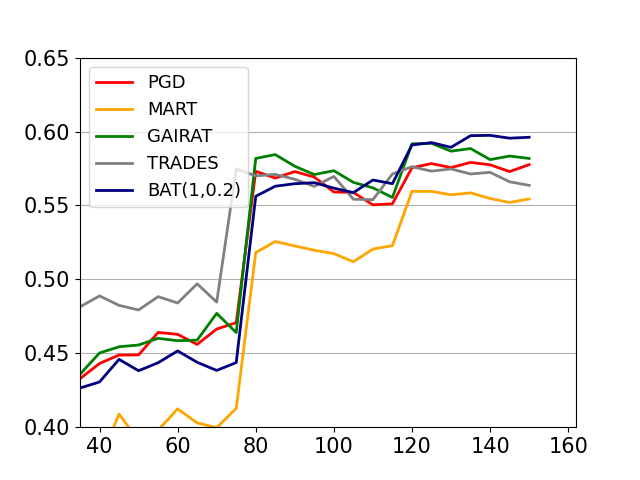
\includegraphics[width = 1.1\textwidth]{figures/base_clean.png}
\end{minipage}
}
\subfloat{
\begin{minipage}[c]{0.3\textwidth}
\centering
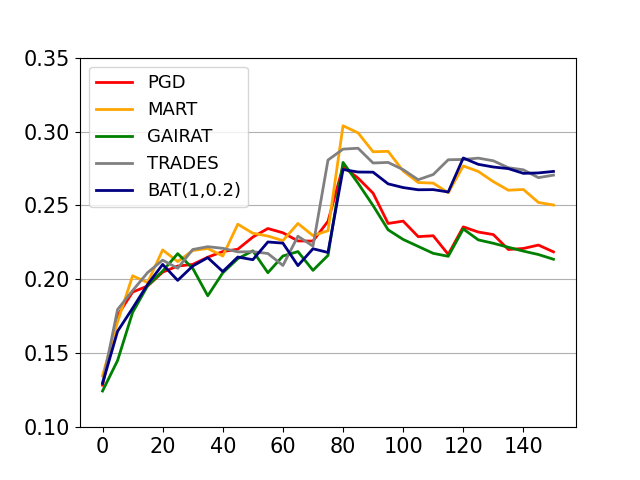
\includegraphics[width = 1.1\textwidth]{figures/base_rob.png}
\end{minipage}
}
\vspace{-0.4cm}
\caption{\small Clean Acc. (left) \& Adv. Acc (right)}
\label{fig:exp1}
\end{wrapfigure}
In Fig.~\ref{fig:exp1}, we also show the change of each models' overall clean accuracy (Fig~\ref{fig:exp1} (left)) \& adversarial accuracy (Fig~\ref{fig:exp1} (right)) along with the training progress. 
Interestingly, similar to PGD adversarial training, all baseline methods cannot achieve the optimal clean and adversarial accuracy at the same moment.
They always achieve the best adversarial accuracy around Epoch 80 (right after the first time weight decay), and the best clean accuracy on the last epochs. However, for BATs, since they can effectively prevent the robustness dropping in the late epochs, BATs are able to train until last epochs and enjoy good clean and adversarial accuracy simultaneously.
%As a result, BATs have higher clean accuracy than all baseline models, and good adversarial accuracy, which are similar or comparable to all baselines (even on their best checkpoints).

\textbf{Performance on Tiny~ImageNet.} Tiny~ImageNet~\cite{le2015tiny} contains 200 classes of the images in the original ImageNet~\cite{krizhevsky2012imagenet} dataset, with 500 training images for each class, and image size $64\times 64$. In our experiments, we only choose the first 50 classes in Tiny ImageNet for training and prediction. Since the image size is $64\times 64$, for both training and robustness evaluation, we consider the adversarial attacks are bounded by $l_\infty$-norm-4/255. In Table~\ref{Tab:results_imagenet}, we report the performance of BAT and baseline methods. Similar to the conclusions we can make from CIFAR100, BATs can achieve the highest overall clean accuracy and comparably good adversarial accuracy with baseline methods. 
\begin{table}[h]
\small
\vspace{-0.2cm}
\centering
\caption{Performance of BAT vs. Baselines on Tiny~ImageNet Under ResNet32}
\begin{tabular}{c|cc|cc|cc}
\hline
Method & All Acc. & All Adv. & Typical Acc. & Typical Adv. & Atyp. Acc. & Atyp. Adv. \\
\hline
\hline
Adv. Train (Best Adv.) & 56.3 & 32.3 & 97.5 & 85.3 &41.5 & 9.6\\
Adv. Train (Best Clean) & 58.2 & 30.5 & 98.0 & 80.4 & 44.7 & 9.1 \\
TRADES ($1/\lambda = 5$) & 55.4 & 28.8 & 97.3 & 77.4 & 38.8 & 9.6 \\
MART~\cite{wang2019improving} & 56.2 & \textbf{34.5} & 97.7 & 85.1 & 41.4 & \textbf{13.6} \\
GAIRAT~\cite{zhang2020geometry} & 58.4 & 30.4 & 98.0 & 81.7 & 45.7 & 7.8\\
\hline
BAT ($\alpha = 1, \beta = 0.2$) & \textbf{59.4} &32.0 & 98.4 & 83.9 & \textbf{48.4} & 10.2 \\
BAT ($\alpha = 2, \beta = 0.2$) &\textbf{59.4} &32.9 & \textbf{99.1} & \textbf{86.9} & 45.7 & 10.9 \\
\hline
\hline
\end{tabular}
\label{Tab:results_imagenet}
\end{table}

\vspace{-0.7cm}
\subsection{Ablation Study}\label{sec:ablation}
\vspace{-0.2cm}
\begin{wrapfigure}{r}{0.6\textwidth}
\vspace{-0.9cm}
\subfloat{
\begin{minipage}[c]{0.32\textwidth}
\centering
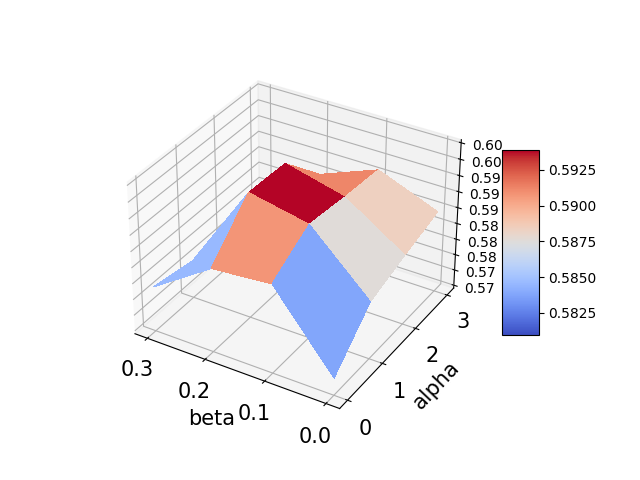
\includegraphics[width = 1.1\textwidth]{figures/abl_clean.png}
\end{minipage}
}
\subfloat{
\begin{minipage}[c]{0.32\textwidth}
\centering
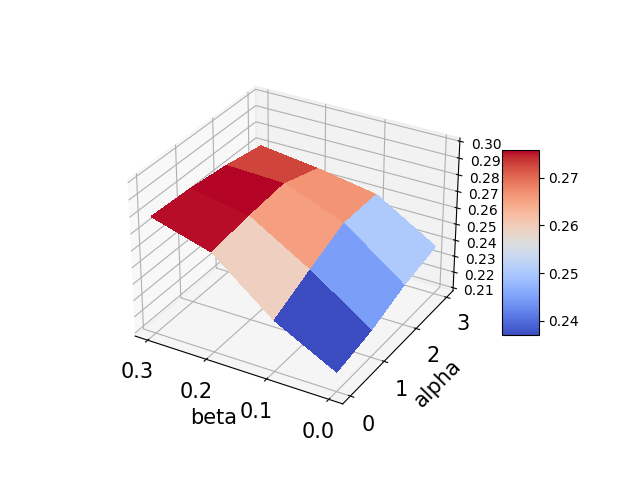
\includegraphics[width = 1.1\textwidth]{figures/abl_rob.png}
\end{minipage}
}
\caption{\small Clean Acc.(left) \& Adv. Acc.(right)}
\label{fig:exp2}
\vspace{-0.2cm}
\end{wrapfigure}
In this subsection, we study the potential impact of the hyperparameters chosen in BAT, which is $\alpha$ that controls the \textit{Reweighting} process and $\beta$ that controls the \textit{Discrimination Loss}. 
In Fig.~\ref{fig:exp2}, we conduct the experiments on CIFAR100 with BAT when $\alpha$ is chosen in [0,1,2,3] and $\beta$ is in [0, 0.1, 0.2, 0.3].
In Fig.~\ref{fig:exp2}, we show each model's overall clean accuracy~(left) \& adversarial accuracy~(right) along the Z-axis, and X-axis / Y-axis indicate the models' corresponding variables of $(\alpha,\beta)$. Note that when $\alpha=\beta=0$, the BAT method regresses to original PGD adversarial training. From the result, we can see that a positive pair of $(\alpha,\beta)$ can benefit both model clean and adversarial accuracy. Therefore, both two components \textit{Reweighting} and \textit{Discrimination Loss} of BAT are helpful and necessary. However, when $\alpha$ or $\beta$ is relatively too large, it will hurt the BAT's clean accuracy. As a result, in CIFAR~100, when $\alpha=1$ or 2 and $\beta= 0.2$, BAT can achieve the optimal performance.

%If we look at the performance of these models at their final epochs, we first observe that $\beta=0.2$ can improve both clean and adversarial accuracy, compared to all models with $\beta = 0$. Moreover, given any fixed value of $\beta$, the model with $\alpha = 1$ or 2 always outperforms than $\alpha=0$.
%Since a positive $\alpha$ indicates the BAT algorithm downweight or exclude certain samples during the training process, we can conclude that those  samples which are downweighted/excluded are acting like poisoning samples to deteriorate the models' performance. and necessary.

\section{Conclusion}
In this work, we advance the method of {machine unlearning} through a novel viewpoint: model sparsification, achieved by weight pruning. We show in both theory and practice that model sparsity plays a foundational and crucial role in closing the gap between exact unlearning and existing approximate unlearning methods. Inspired by that, we propose two new unlearning paradigms,  `prune first, then unlearn' and `sparsity-aware unlearn', which can significantly improve the efficacy of approximate unlearning. We demonstrate the effectiveness of our findings and proposals in extensive experiments across different unlearning setups. Our study also indicates the presence of \textit{model modularity} traits, such as weight sparsity, that could simplify the process of machine unlearning. This may open up exciting prospects for future research to investigate unlearning patterns within weight or architecture space.






\bibliography{main}
\newpage
\appendix
\onecolumn
\begin{algorithm}[t!]
\small
	\caption{Proposed {\myalgo} Algorithm}\label{algo:localstep01}
	\begin{algorithmic}[1]
		\Require local model on the $i$-th node $\*x^{(i)}_{0}$, learning rate $\{\gamma_t\}_{t=1}^{T}$, $\*m_0=\*0$, $\*v_0=\*0$, auxiliary buffer $\*u_0=\*0$, total number of iterations $T$, decaying factor $\beta_1$, $\beta_2$ from Adam, numerical constant $\epsilon$, variance update step index set $\mathcal{T}_{\*v}$, synchronization step index set $\mathcal{T}_{\*u}$, the most recent step with synchronization $t'=0$.
		\For{$t=0, \cdots, T-1$}
		    \State Compute local stochastic gradient $\*g^{(i)}_t$.
		    \State Update momentum: $\*m^{(i)}_{t+\frac{1}{2}} = \beta_1\*m^{(i)}_{t} + (1-\beta_1){\*g}^{(i)}_t$.
		    \State Update model: $\*x^{(i)}_{t+\frac{1}{2}} = \*x^{(i)}_{t} - \gamma_t{\*m}^{(i)}_t/\sqrt{\*v_t+\epsilon}$.
		    \State Update buffer: $\*u^{(i)}_{t+\frac{1}{2}} = \*u^{(i)}_{t} + \gamma_t{\*m}^{(i)}_t$.
		    \If{$t\in\mathcal{T}_{\*u}$}
    		    \State Perform 1-bit AllReduce: $\overline{\*u}_{t+\frac{1}{2}}$ = \textbf{1bit-AllReduce} $\left(\*u_{t+\frac{1}{2}}^{(i)}\right)$.
    		    \State Approximate momentum with compressed buffer: $\*m^{(i)}_{t+1} = \overline{\*u}_{t+\frac{1}{2}}/\sum_{h=t'}^{t}\gamma_h$.
    		    \State Update model with compressed buffer: $\*x^{(i)}_{t+1} = \*x^{(i)}_{t'} - \overline{\*u}_{t+\frac{1}{2}}/\sqrt{\*v_t+\epsilon}$.
    		    \State Reset the auxiliary buffer: $\*u^{(i)}_{t+1} = \*0$.
    		    \State Update the synchronization step: $t'=t$.
    		\Else
    		    \State  $\*x^{(i)}_{t+1}=\*x^{(i)}_{t+\frac{1}{2}}$; $\*m^{(i)}_{t+1}=\*m^{(i)}_{t+\frac{1}{2}}$; $\*u^{(i)}_{t+1}=\*u^{(i)}_{t+\frac{1}{2}}$.
    	    \EndIf
    	    \If{$t\in\mathcal{T}_{\*v}$}
		        \State Perform full-precision AllReduce: $\overline{\*g}_t$ = \textbf{AllReduce} $\left(\*g_t^{(i)}\right)$.
		        \State Update the variance: $\*v_{t+1} = \beta_2\*v_{t} + (1-\beta_2)(\overline{\*g}_t)^2$.
		    \Else
		        \State Use the stale variance for the next iteration: $\*v_{t+1} = \*v_{t}$.
		    \EndIf
		\EndFor
		\State \textbf{return} $\*x_T$.
	\end{algorithmic}
\end{algorithm}

\section{\myalgo}
\label{sec:algorithm}
% \minjia{Not sure if this is the best section title we can come up with. It describes what we did but (1) fixing something feels a bit incremental, and (2) it does not connect very well with the title of our paper, where we pitch 0/1 Adam as a technique for maximizing the communication efficiency. Maybe: Extreme Compression with Linear Approximation for Addressing Non-Linearity in Adam? Not my favorite as it is too long, but hopefully this helps you to come up with a better section title.}
In this section, we give the full description of {\myalgo}. To maximize the communication efficiency, ideally we want an algorithm that enables adaptive convergence like Adam, while allowing aggressive compression (e.g. 1 bit) and requires no additional synchronization on the optimizer states when using local steps. {\myalgo} solves this problem from two aspects.

\textbf{Adaptive Variance Freezing.}
To begin with,
{\myalgo} creates a linear environment that freezes the variance adaptively. The intuition is leveraged from the observation in Figure~\ref{fig:profile_bert_large:var_diff_time}: the change of variance over steps in Adam is generally smooth. While 1-bit Adam captures a reasonable variance estimate via one-time freezing, it is reasonable to also presume that before its freezing point, the variance within several adjacent steps will stay close due to its smoothness.
This motivates us to extend the one-time freezing policy in 1-bit Adam into an adaptive one, by letting workers agree upon the freezing points from a given step index set $\mathcal{T}_{\*v}\subseteq\{0, \cdots, T-1\}$.
The frozen variance creates multiple intervals over training, during which the workers have agreement on the denominator (Equation~(\ref{equa:Adam_update})) and the only uncertainty is then left in the nominator that is linearly dependent on the model update, just like SGD.

% We provide the formal description of this idea in Algorithm~\ref{algo:basic01}, from which the 1-bit Adam can then be viewed as a special case of setting $\mathcal{T}_{\*v}=\{0, \cdots, T_0-1\}$.

% \textbf{Skipping communication rounds requires states synchronization.}
% As will be shown in Section~\ref{sec:experiment}, while a well-constructed $\mathcal{T}_{\*v}$ is able to reduce the per-parameter volume towards 1 bit, its end-to-end throughput improvement is limited. This happens since, as illustrated in Section~\ref{sec:motivation}, the fixed cost of initiating communication rounds and compression is non-negligible.
% This further motivates us to let Algorithm~\ref{algo:basic01} work with skipped communication rounds so as to maximize its communication efficiency.
% As shown in previous works, performing local steps (i.e. skipping rounds) in Adam requires synchronization on the optimizer states \citep{yu2019linear,chen2021convergence}. Specifically, since local gradients computed on each worker are different, without periodic synchronization the optimizer states on different workers will diverge from each other. As shown in Figure~\ref{fig:profile_bert_large:mom_diff_local} and \ref{fig:profile_bert_large:var_diff_local}, the difference between local and global optimizer states, momentum and variance, remain constants and do not decrease to zero. The additional synchronization on momentum and variance could potentially compromise the performance gain from applying local steps.

\textbf{Including 1-bit Compression and Local Steps.}
% Ideally, we want a strategy that lets all the workers reach consensus on optimizer states without incurring new communication volume. Denote $\*x_t^{(i)}$, $\*m_t^{(i)}$, $\*v_t^{(i)}$ as the model, momentum, variance on worker $i$ at step $t$, respectively. Suppose all the workers are synchronized at step $t'$, and skip all the communication rounds to step $t$, we obtain for any $i\in\{1, \cdots, n\}$,
% \begin{align*}
%     \*x_t^{(i)} = \*x_{t'}^{(i)} - \sum_{k=t'}^{t-1}\frac{\gamma_k\*m_k^{(i)}}{\sqrt{\*v_k^{(i)}+\epsilon}}.
% \end{align*}
% Since directly applying 1-bit compression to model parameters can easily cause divergence \citep{basu2020qsparse}, we instead apply compression to $\*x_t^{(i)} - \*x_{t'}^{(i)}$ (which we refer to as model difference) given that all the workers have agreed on $\*x_{t'}^{(i)}$. Compressing the model difference, on one hand, makes the compression error bounded since when the algorithm converges, the model difference will generally approach zero; on the other hand, it provides the opportunity for us to synchronize optimizer states for free as illustrated next.
% The main design of 1-bit sync is leveraged from the following observation: if all the workers use the same frozen variance during a sequence of local steps, then 
With frozen variance, we make another observation based on Equation~(\ref{equa:Adam_update}) that the model difference on workers will be linearly dependent to the momentum. So that, the momentum can be approximated locally rather than synchronized additionally based on the communicated model difference, given the premise that the change of momentum is not abrupt within close steps. Formally, denote $\*x_t^{(i)}$, $\*m_t^{(i)}$, $\*v_t^{(i)}$ as the model, momentum, variance on worker $i$ at step $t$, respectively. Suppose all the workers are synchronized at step $t'$, then with frozen variance $\*v$ over all the workers,
\begin{align*}
\*u_t^{(i)} &= \sum\nolimits_{k=t'}^{t}\gamma_k\*m_k^{(i)} && \text{Actual sent tensors in the communication.} \\
\*x_{t+1}^{(i)} &= \*x_{t'}^{(i)} - \frac{1/n\sum\nolimits_{i=1}^{n}\*u_t^{(i)}}{\sqrt{\*v+\epsilon}} && \text{Sync model parameters with the sent tensors.} \\
\*m_{t+1}^{(i)} &\approx \frac{1/n\sum\nolimits_{i=1}^{n}\*u_t^{(i)}}{\sum\nolimits_{k=t'}^{t}\gamma_k} && \text{Approximate momentum via linear estimates via sent tensor.}
\end{align*}
where we omit the compression part for brevity.
Combined with compression, we provide the full description of {\myalgo}\footnote{The name comes from the fact that the algorithm can potentially reduce the per-parameter volume to some number between 0 and 1 bit on average.} in Algorithm~\ref{algo:localstep01}.
Note that here we defer the details of 1-bit compression to Appendix~\ref{appendix:sec:algorithm} and treat it as a black-box procedure named \textbf{1bit-AllReduce} while the original full-precision AllReduce is referred to as \textbf{AllReduce}. 

We also remark that although both techniques appear to be natural, to the best of our knowledge,  we are the first to apply them to addressing the non-linearity challenges in 1-bit compression and local steps for maximizing the communication efficiency of Adam optimizer.  


% \textbf{Techniques in {\myalgo} are correlated.}
% Giving a closer look at Algorithm~\ref{algo:localstep01}, all the techniques are not orthogonally combined but are highly correlated. In fact, the approximation in 1-bit sync cannot be performed accurately if the variance during the local steps are different. On the other hand, compressing model difference rather than model itself also makes the momentum approximation possible due to their linear dependency.


\vspace{-0.2cm}
\section{Experiment}\label{sec:exp}
\vspace{-0.2cm}
In this section, we present the experimental results to validate the effectiveness of the proposed BAT algorithm on benchmark datasets and compare it with state-of-the-art baseline methods. We also verify that both two components are helpful and necessary for BAT. The implementation of the BAT can be found via \url{https://anonymous.4open.science/r/benign-adv-77C5}.

\vspace{-0.2cm}
\subsection{Experimental Setup}
\vspace{-0.1cm}
%\jt{we can put baselines here.} \\
%\jt{implementation details, such as optimization method}
In this work, in order to demonstrate the 
merit of BAT, we conduct the experiments mainly on benchmark datasets CIFAR100~\cite{krizhevsky2009learning} and Tiny~ImageNet~\cite{le2015tiny}, which are relatively complex datasets (i.e., containing larger fractions of atypical samples). For both datasets, we study the algorithms under the model architectures ResNet and WideResNet (WRN)~\cite{he2016deep}. In this section, we only present the results of ResNet18 for CIFAR100 and ResNet32 for Tiny~ImageNet and leave the results on WRN in Appendix~\ref{app:exp}. As a fair comparison with BAT, we implement the baseline algorithms including PGD adversarial training~\cite{madry2017towards} as well as its most popular variant TRADES~\cite{zhang2019theoretically}. In addition, we include several recent algorithms: MART~\cite{wang2019improving} and GAIRAT~\cite{zhang2020geometry}, which also incorporate reweighting strategies into adversarial training. For BAT and all baseline methods, we run the algorithms using SGD~\cite{bottou2010large} for 160 epochs with the learning rate that starts from 0.1 and decays by 0.1 after the epoch 80 and 120. More implementation details can be found in Appendix~\ref{app:exp}.

\textbf{Performance on CIFAR100.} For a comprehensive comparison between different methods on CIFAR100, in the results from Table~\ref{Tab:results_cifar100}, we report the models' clean accuracy and adversarial accuracy against $l_\infty$-$8/255$ PGD attack~\cite{madry2017towards}, as well as their performance on the typical sample set and atypical sample set (as described in Section~\ref{sec:pre}). A more comprehensive robustness evaluation on different attacking methods (including CW~\cite{carlini2017towards} and Auto-Attack~\cite{croce2020reliable}) are presented in Appendix~\ref{app:exp}. For BAT, we report its performance when choosing its optimal hyperparameter: $\alpha = 1  ~\text{\&} ~2$ and $\beta = 0.2$. In the Section~\ref{sec:ablation}, we will discuss the impact of the selection of $\alpha$ and $\beta$ on BAT. For baseline methods, the settings and checkpoint selections follow the original papers' suggestions.

%Note that the main goal of BAT is not to improve model's adversarial robustness, so we leave the robustness evaluation with additional attacking methods, such as CW~\cite{carlini2017towards} and Auto Attack~\cite{croce2020reliable} in  Appendix~\ref{app:exp} where we have similar observations.

\vspace{-0.3cm}
\begin{table}[h]
\small
\centering
\caption{Performance of BAT vs. Baselines on CIFAR100 Under ResNet18}
\begin{tabular}{c|cc|cc|cc}
\hline
Method & All Acc. & All Adv. & Typical Acc. & Typical Adv. & Atyp. Acc. & Atyp. Adv. \\
\hline
\hline
PGD Train (Best Adv.) & 56.9 & 27.4 & 90.6 & 59.0 &29.5 & 7.7\\
PGD Train (Best Clean) & 57.8 & 21.9 & 88.3 & 51.0 & \textbf{40.1} & 8.3 \\
%TRADES ($1/\lambda = 1$) & \textbf{61.3} & 21.9 & \textbf{93.0} & 50.0 & 44.7 & 7.9\\
TRADES ($1/\lambda = 5$) & 56.6 & 26.9 & 88.9 & 57.1 & 37.3 & \textbf{10.9} \\
MART~\cite{wang2019improving} & 51.8 & \textbf{30.4} & 85.3 & \textbf{62.2} & 25.3 & 10.1\\
GAIRAT~\cite{zhang2020geometry} & 58.2 & 27.8 & 90.6 & 60.7 & 31.6 & 8.2\\
\hline
BAT ($\alpha = 1, \beta = 0.2$) & \textbf{59.5} &27.3 & \textbf{92.3} & 58.8 & 36.3 & 8.7 \\
BAT ($\alpha = 2, \beta = 0.2$) &59.3 & 27.4 & \textbf{92.3} & 60.3 & 33.1 & 7.4 \\
\hline
\hline
\end{tabular}
\label{Tab:results_cifar100}
\end{table}
\vspace{-0.2cm}
From the results in Table~\ref{Tab:results_cifar100}, we can find that BATs enjoy good clean \& adversarial accuracy trade-off among all methods. It is because BATs can obtain the highest overall clean accuracy ($\sim59.5\%$), as well as comparably good adversarial accuracy ($\sim27.3$) with baseline methods. The only exception is MART~\cite{wang2019improving} which has the higher adversarial accuracy around $\sim 30\%$. However, MART~\cite{wang2019improving} has much lower clean accuracy than BATs. 

To gain a deeper understanding of the working mechanism of BAT, we focus on the performance on BAT vs. PGD adversarial training~\cite{madry2017towards}. Compared with PGD adversarial training with highest adversarial accuracy (PGD Train (Best Adv.)), the BAT methods are $2\sim3\%$ higher in terms of overall clean accuracy, and similar adversarial accuracy. The improvement of clean accuracy is mainly due to BATs' capacity to fit much more atypical samples. For example, the clean accuracy of BAT ($\alpha=1, \beta=0.2$) is about $6\%$ higher than PGD Train~(Best Adv.). On the other hand, compared to PGD adversarial training with the highest clean accuracy (PGD Train (Best Clean)), BATs have much better overall adversarial robustness and slightly better clean accuracy. This is mainly due to BAT's advantage on typical samples, because BATs can successfully prevent the performance drop of typical samples during the training process. Since BATs can achieve good performance on both typical samples and atypical samples, BATs outperform PGD adversarial training in CIFAR100.

\begin{wrapfigure}{r}{0.6\textwidth}
\vspace{-0.4cm}
\subfloat{
\begin{minipage}[c]{0.3\textwidth}
\centering
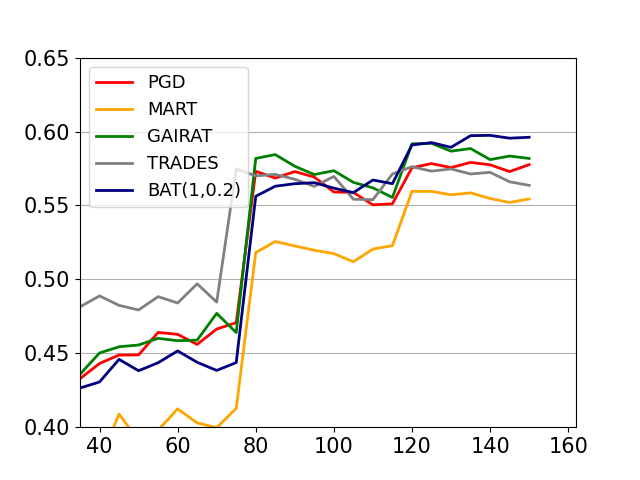
\includegraphics[width = 1.1\textwidth]{figures/base_clean.png}
\end{minipage}
}
\subfloat{
\begin{minipage}[c]{0.3\textwidth}
\centering
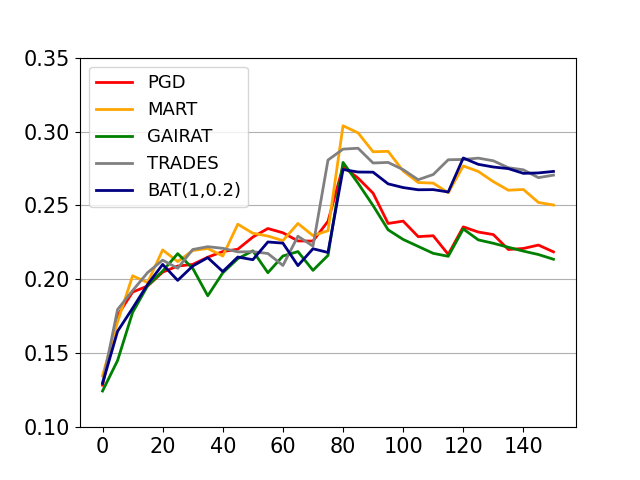
\includegraphics[width = 1.1\textwidth]{figures/base_rob.png}
\end{minipage}
}
\vspace{-0.4cm}
\caption{\small Clean Acc. (left) \& Adv. Acc (right)}
\label{fig:exp1}
\end{wrapfigure}
In Fig.~\ref{fig:exp1}, we also show the change of each models' overall clean accuracy (Fig~\ref{fig:exp1} (left)) \& adversarial accuracy (Fig~\ref{fig:exp1} (right)) along with the training progress. 
Interestingly, similar to PGD adversarial training, all baseline methods cannot achieve the optimal clean and adversarial accuracy at the same moment.
They always achieve the best adversarial accuracy around Epoch 80 (right after the first time weight decay), and the best clean accuracy on the last epochs. However, for BATs, since they can effectively prevent the robustness dropping in the late epochs, BATs are able to train until last epochs and enjoy good clean and adversarial accuracy simultaneously.
%As a result, BATs have higher clean accuracy than all baseline models, and good adversarial accuracy, which are similar or comparable to all baselines (even on their best checkpoints).

\textbf{Performance on Tiny~ImageNet.} Tiny~ImageNet~\cite{le2015tiny} contains 200 classes of the images in the original ImageNet~\cite{krizhevsky2012imagenet} dataset, with 500 training images for each class, and image size $64\times 64$. In our experiments, we only choose the first 50 classes in Tiny ImageNet for training and prediction. Since the image size is $64\times 64$, for both training and robustness evaluation, we consider the adversarial attacks are bounded by $l_\infty$-norm-4/255. In Table~\ref{Tab:results_imagenet}, we report the performance of BAT and baseline methods. Similar to the conclusions we can make from CIFAR100, BATs can achieve the highest overall clean accuracy and comparably good adversarial accuracy with baseline methods. 
\begin{table}[h]
\small
\vspace{-0.2cm}
\centering
\caption{Performance of BAT vs. Baselines on Tiny~ImageNet Under ResNet32}
\begin{tabular}{c|cc|cc|cc}
\hline
Method & All Acc. & All Adv. & Typical Acc. & Typical Adv. & Atyp. Acc. & Atyp. Adv. \\
\hline
\hline
Adv. Train (Best Adv.) & 56.3 & 32.3 & 97.5 & 85.3 &41.5 & 9.6\\
Adv. Train (Best Clean) & 58.2 & 30.5 & 98.0 & 80.4 & 44.7 & 9.1 \\
TRADES ($1/\lambda = 5$) & 55.4 & 28.8 & 97.3 & 77.4 & 38.8 & 9.6 \\
MART~\cite{wang2019improving} & 56.2 & \textbf{34.5} & 97.7 & 85.1 & 41.4 & \textbf{13.6} \\
GAIRAT~\cite{zhang2020geometry} & 58.4 & 30.4 & 98.0 & 81.7 & 45.7 & 7.8\\
\hline
BAT ($\alpha = 1, \beta = 0.2$) & \textbf{59.4} &32.0 & 98.4 & 83.9 & \textbf{48.4} & 10.2 \\
BAT ($\alpha = 2, \beta = 0.2$) &\textbf{59.4} &32.9 & \textbf{99.1} & \textbf{86.9} & 45.7 & 10.9 \\
\hline
\hline
\end{tabular}
\label{Tab:results_imagenet}
\end{table}

\vspace{-0.7cm}
\subsection{Ablation Study}\label{sec:ablation}
\vspace{-0.2cm}
\begin{wrapfigure}{r}{0.6\textwidth}
\vspace{-0.9cm}
\subfloat{
\begin{minipage}[c]{0.32\textwidth}
\centering
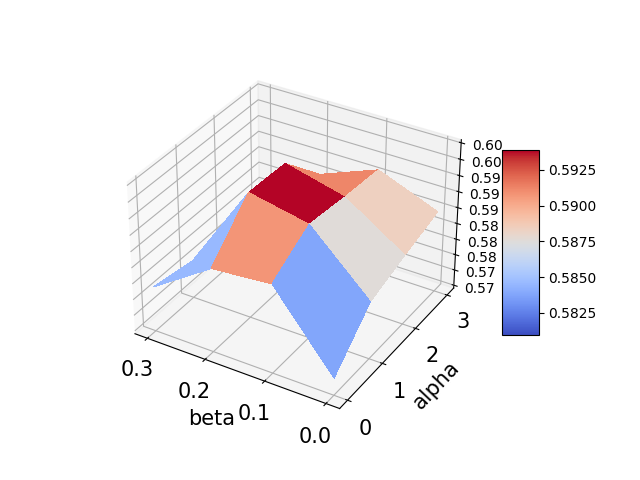
\includegraphics[width = 1.1\textwidth]{figures/abl_clean.png}
\end{minipage}
}
\subfloat{
\begin{minipage}[c]{0.32\textwidth}
\centering
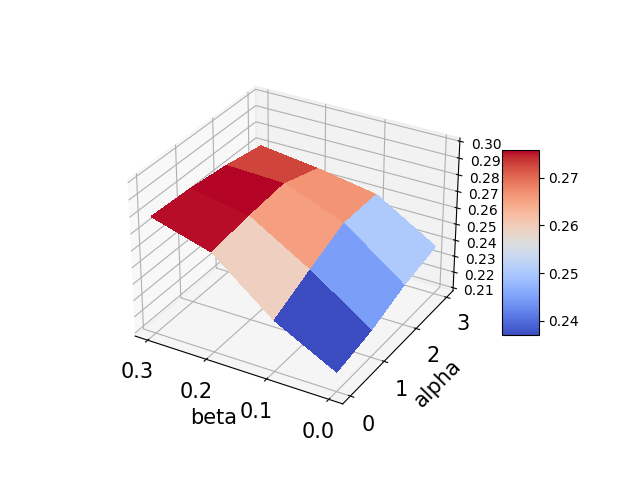
\includegraphics[width = 1.1\textwidth]{figures/abl_rob.png}
\end{minipage}
}
\caption{\small Clean Acc.(left) \& Adv. Acc.(right)}
\label{fig:exp2}
\vspace{-0.2cm}
\end{wrapfigure}
In this subsection, we study the potential impact of the hyperparameters chosen in BAT, which is $\alpha$ that controls the \textit{Reweighting} process and $\beta$ that controls the \textit{Discrimination Loss}. 
In Fig.~\ref{fig:exp2}, we conduct the experiments on CIFAR100 with BAT when $\alpha$ is chosen in [0,1,2,3] and $\beta$ is in [0, 0.1, 0.2, 0.3].
In Fig.~\ref{fig:exp2}, we show each model's overall clean accuracy~(left) \& adversarial accuracy~(right) along the Z-axis, and X-axis / Y-axis indicate the models' corresponding variables of $(\alpha,\beta)$. Note that when $\alpha=\beta=0$, the BAT method regresses to original PGD adversarial training. From the result, we can see that a positive pair of $(\alpha,\beta)$ can benefit both model clean and adversarial accuracy. Therefore, both two components \textit{Reweighting} and \textit{Discrimination Loss} of BAT are helpful and necessary. However, when $\alpha$ or $\beta$ is relatively too large, it will hurt the BAT's clean accuracy. As a result, in CIFAR~100, when $\alpha=1$ or 2 and $\beta= 0.2$, BAT can achieve the optimal performance.

%If we look at the performance of these models at their final epochs, we first observe that $\beta=0.2$ can improve both clean and adversarial accuracy, compared to all models with $\beta = 0$. Moreover, given any fixed value of $\beta$, the model with $\alpha = 1$ or 2 always outperforms than $\alpha=0$.
%Since a positive $\alpha$ indicates the BAT algorithm downweight or exclude certain samples during the training process, we can conclude that those  samples which are downweighted/excluded are acting like poisoning samples to deteriorate the models' performance. and necessary.

\section{Additional Experimental Details}
\label{appendix:sec:exp}
\textbf{Training Parameters.}
For BERT pretraining, we follow the settings from \citep{devlin2018bert} and let the learning rate linearly increases to $4\times 10^{-4}$ as a warmup in the first 12.5K steps, then decays into 0.99 of the original after
every 520 steps. We set $\beta_1=0.9$ and $\beta_2=0.999$ for all the algorithms. We adopt the batch size of 4096. For 1-bit Adam, we follow the hyperparameters given in \citep{tang20211} and set the full-precision stage for 1-bit Adam as 16K and 23K on BERT-Base and BERT-Large, respectively. 
All the hyperparameters used here (e.g. learning rate) strictly follow \citep{tang20211} for fair comparison.
For ImageNet, we follow the example script from Pytorch\footnote{\url{https://github.com/pytorch/examples/blob/master/imagenet/main.py}} and use batch size of 256 and a milestone decay learning rate schedule: starting at 1e-4 and decay by a factor of 10 at epoch 30 and 60, with 90 epochs in total. We set 10 epochs (50050 steps) as the full-precision stage for 1-bit Adam.
For GPT-2 we set batch size to be 512, and use 300K training steps (158B tokens). The learning rate schedule follows a linear warmup of 3K steps and a single cycle consine decay over the remaining 297K steps ($1\times 10^{-5}\min$). For 1-bit Adam, we set its full-precision stage length to be 80K steps, and for the {\myalgo}, we follow the same learning rate based policy from BERT on $\mathcal{T}_{\*v}$ and $\mathcal{T}_{\*u}$. 

For GLUE benchmarks we use Adam optimizer and perform single-task training on the dev set. Following the setup in the BERT paper~\citep{devlin2018bert} and 1-bit Adam paper \citep{tang20211}, we search over the hyperparameter space with batch sizes $\in\{8,16,32\}$ and learning rates $\{1\times 10^{-5},3\times 10^{-5},5\times 10^{-5},8\times 10^{-5}\}$.

The convergence plots for GPT-2 pre-training are given in Figure~\ref{exp:fig:gpt_converge}.
\begin{figure}[t!]
  \centering
  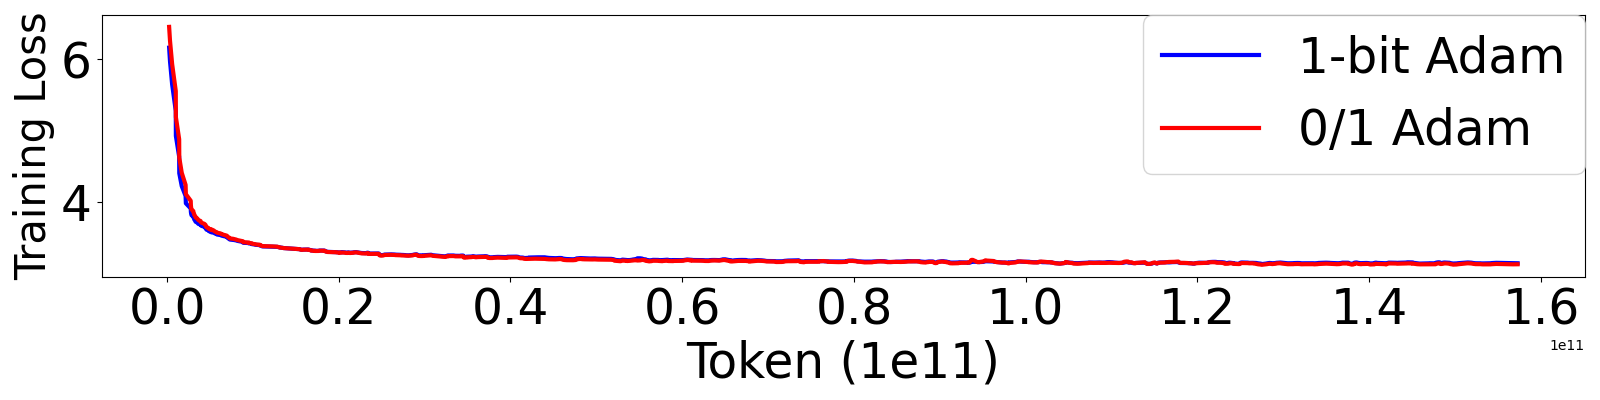
\includegraphics[width=0.49\textwidth]{./sections/figure/v3_gpt2_sample.png}
  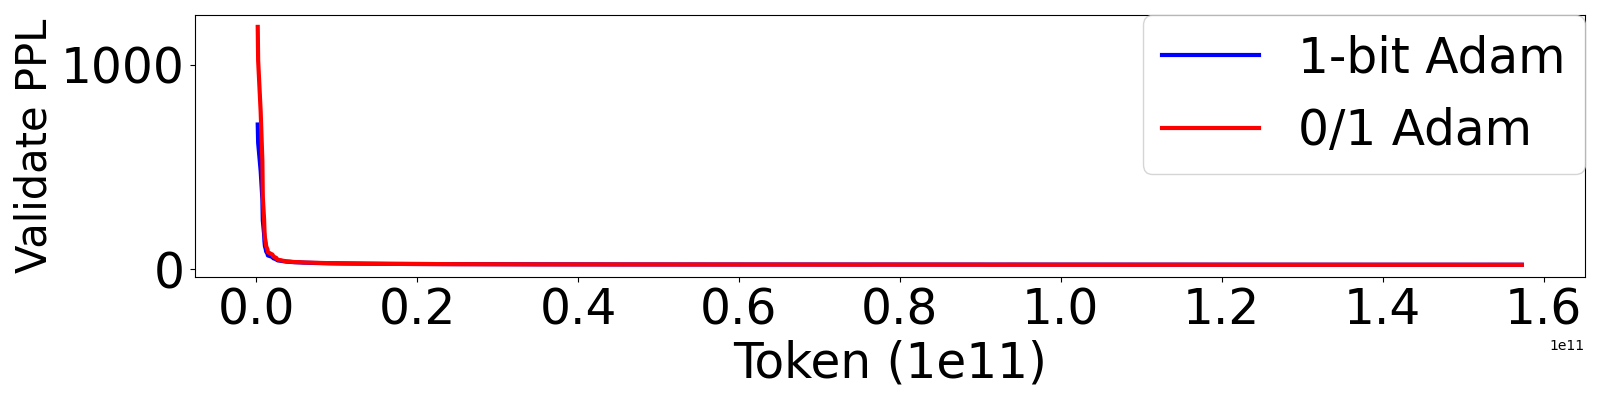
\includegraphics[width=0.49\textwidth]{./sections/figure/v3_gpt2_val.png}
  \caption{Training loss (left) and validation perplexity (right) with respect to Tokens for 1-bit Adam and {\myalgo}.}
  \label{exp:fig:gpt_converge}
\end{figure}

% Figure~\ref{exp:fig:gpt_converge} shows that {\myalgo} is able to achieve the same convergence speed as 1-bit Adam with less communication rounds and bits per parameters, which is aligned with our findings on BERT and ImageNet tasks. Table~\ref{exp:table:gpt} summarizes the quality of output models via zero-shot tasks over WikiText-103 and LAMBADA datasets. We observe {\myalgo} is able to achieve the comparable perplexity and accuracy with Adam, while higher than 1-bit Adam.

% \begin{table}[h!]
%   \centering
%   \caption{Zero-shot evaluation of the trained models on WikiText-103 and LAMBADA datasets, the evaluation methodology follows \citep{shoeybi2019megatron}. The number for Adam is obtained from \citep{li2021curriculum}.}
%   \label{exp:table:gpt}
%   \begin{tabular}{lccccccccc}
%   \hline  
%   & WikiText Perplexity $\downarrow$ & LAMBADA accuracy $\uparrow$ \\
%   \hline 
%   Adam & 27.78 & 33.19 \\
%   1-bit Adam & 28.37 & 33.21 \\
%   {\myalgo} & 28.07 & 33.51 \\
%   \hline
%   \end{tabular}
% \end{table}
\section{Theoretical Analysis}
\label{appendix:sec:proof}
\subsection{Analysis to an intermediate version of {\myalgo}}
\begin{algorithm}[ht!]
\small
	\caption{Generic framework of applying 1-bit communication to Adam with frozen variance state. 1-bit Adam can be viewed as a special case of setting $\mathcal{T}_{\*v}=\{0,\cdots,T_0-1\}$ where $T_0$ denotes its total number of steps in the full-precision stage.}\label{algo:basic01}
	\begin{algorithmic}[1]
		\Require initialized model on worker $i$: $\*x_{0}^{(i)}$, learning rate $\{\gamma_t\}_{t=1}^{T}$, $\*m_0=\*0$, $\*v_0=\*0$, total number of iterations $T$, decaying factor $\beta_1$, $\beta_2$ from Adam, numerical constant $\epsilon$, variance update step index set $\mathcal{T}_{\*v}$.
		\For{$t=0, \cdots, T-1$}
		    \State Locally compute stochastic gradient $\*g^{(i)}_t$ over $\*x_{t}^{(i)}$.
		    \If{$t\in\mathcal{T}_{\*v}$}
		        \State $\overline{\*g}_t$ = \textbf{AllReduce} $\left(\*g_t^{(i)}\right)$.
		        \State Set $\*v_{t+1} = \beta_2\*v_{t} + (1-\beta_2)(\overline{\*g}_t)^2$.
		    \Else
		        \State $\overline{\*g}_t$ = \textbf{Compressed-AllReduce} $\left(\*g_t^{(i)}\right)$.
		        \State Set $\*v_{t+1} = \*v_{t}$.
		    \EndIf
		    \State Update momentum: $\*m_{t+1} = \beta_1\*m_{t} + (1-\beta_1)\overline{\*g}_{t}$.
		    \State Update model: $\*x_{t+1}^{(i)} = \*x_{t}^{(i)} - \gamma_t\*m_{t}/\sqrt{\*v_{t}+\epsilon}$.
		\EndFor
		\State \textbf{return} $\*x_T^{(i)}, \forall i$.
	\end{algorithmic}
\end{algorithm}
We start from a special case of {\myalgo} that compresses gradients without local steps. This is given in Algorithm~\ref{algo:basic01}.
Note that the following proof will use Algorithm~\ref{algo:EF} to replace \textbf{Compressed-AllReduce} in Algorithm~\ref{algo:basic01}, as introduced in Section~\ref{appendix:sec:algorithm}.

Algorithm~\ref{algo:basic01} allows us to work with weaker assumption as given in the following
\begin{assumption}
\label{assume:compression}
\textbf{Compression error in Algorithm~\ref{algo:basic01}:}
    For arbitrary $\*x\in\mathbb{R}^d$, there exists a constant $0\leq \omega < 1$, such that the output of compressor $\mathcal{C}[\cdot]$ has the following error bound:
    \begin{align*}
        \mathbb{E}\left\| \mathcal{C}[\*x] - \*x \right\|^2 \leq \omega \left\| \*x\right\|^2.
    \end{align*}
\end{assumption}

\begin{restatable}{thm}{thmzerooneadambasic}
\label{thm:basic01}
Under Assumption~\ref{assum:smooth}, \ref{assume:variance}, \ref{assume:g_bound}, and \ref{assume:compression}, let $m=|\mathcal{T}_{\*v}|$, and select $\beta_1, \beta_2\in[0,1)$ such that $m\leq\log(1-\beta_1)/\log(\beta_2)$.
If we run Algorithm~\ref{algo:basic01} with a constant learning rate: for all $t\geq 0$
\begin{align*}
    \gamma_t = \min\left\{ \sqrt{\frac{n}{\sigma^2T}}, \frac{1}{2L\sqrt{G_\infty^2+\epsilon}}, \frac{1}{125}  \right\},
\end{align*}
then it holds that
\begin{align*}
    \frac{1}{T}\sum_{t=0}^{T-1} \mathbb{E}\|\nabla f(\*x_t)\|^2 \leq O\left( \frac{\sigma}{\sqrt{nT}} + \frac{m+n}{(1-\omega)^4T} +\frac{1}{T}\right),
\end{align*}
where we omit $f(\*0)-\inf_{\*x\in\mathbb{R}^d}f(\*x)$,  $G_\infty$, $d$, $\epsilon$, $\beta_1$, $\beta_2$ and $L$ as constants.
\end{restatable}

\begin{proof}
The main update of Algorithm~\ref{algo:basic01} (with constant learning rate) can be summarized as: for every $t=0, \cdots, T-1$,
\begin{align*}
    \*m_{t+1} & = \beta_1\*m_{t} + (1-\beta_1)\overline{\*g}_t \\
    \*v_{t+1} & = \left\{
    \begin{array}{ll}
        \beta_2\*v_{t} + (1-\beta_2)\left( \frac{1}{n}\sum_{i=1}^{n}\*g^{(i)}_t \right)^2 & t\in\mathcal{T}_{\*v}, \\
        \\
        \*v_{t} & t\not\in\mathcal{T}_{\*v}. \\
    \end{array}\right. \\
    \*x_{t+1} & = \*x_{t} - \gamma \frac{\*m_t}{\sqrt{\*v_t +  \epsilon} },
\end{align*}
where the $\overline{\*g}_t$ is the output of the \textbf{1-bit AllReduce} algorithm\footnote{In the original Algorithm~\ref{algo:basic01}, the $\overline{\*g}_t$ is the output of the \textbf{AllReduce} when $t\in\mathcal{T}_{\*v}$. This, however, does not affect our analysis, since our proof holds for a noisier case. The original Algorithm~\ref{algo:basic01} is mainly for practical concern -- we avoid redundant \textbf{AllReduce} rounds when \textbf{1-bit AllReduce} is performed.}.
Note that based on Algorithm~\ref{algo:EF}, the gradient approximation term follows:
\begin{align*}
    \overline{\*g}_{t} = & \frac{1}{n}\sum_{i=1}^{n}\hat{\*g}^{(i)}_{t} + \overline{\*\delta}_{t} - \overline{\*\delta}_{t+1} \\
        = & \frac{1}{n}\sum_{i=1}^{n}\left( \*g^{(i)}_{t} + \*\delta^{(i)}_{t} - \*\delta^{(i)}_{t+1} \right) + \overline{\*\delta}_{t} - \overline{\*\delta}_{t+1} \\
    = & \frac{1}{n}\sum_{i=1}^{n}\*g^{(i)}_{t} + \left( \frac{1}{n}\sum_{i=1}^{n}\*\delta^{(i)}_{t} - \overline{\*\delta}_{t}\right) - \left( \frac{1}{n}\sum_{i=1}^{n}\*\delta^{(i)}_{t+1} - \overline{\*\delta}_{t+1}\right) \\
        = & \*g_t + \*\delta_{t} - \*\delta_{t+1},
\end{align*}
where we denote
\begin{align*}
    \*g_t = & \frac{1}{n}\sum_{i=1}^{n}\*g^{(i)}_t \\
    \*\delta_{t} = & \frac{1}{n}\sum_{i=1}^{n}\*\delta^{(i)}_{t} - \overline{\*\delta}_{t}.
\end{align*}
To prove the convergence, we now
define the following auxiliary sequence: for any $t\geq 0$,
\begin{align*}
    \*y_t = \*x_t - \frac{\gamma\*m_t}{(1-\beta_1)\sqrt{\*v_{t}+\epsilon}} - \frac{\gamma\*\delta_{t}}{\sqrt{\*v_{t}+\epsilon}}.
\end{align*}
The rest of the proof is to use this auxiliary sequence to bound two types of steps separately. We call a step $t$ as \emph{reuse step} if $t\not\in\mathcal{T}_{\*v}$ and \emph{update step} otherwise. We see for all the update steps, $\*v_{t}\neq\*v_{t+1}$ while for all the reuse steps $\*v_{t}=\*v_{t+1}$. 
The bounds on two different types of steps are provides by Lemma~\ref{lemma:reuse_step} and Lemma~\ref{lemma:update_step}. Specifically, denoting $V_1 = \left\| \frac{1}{\sqrt{\*v_1+\epsilon}}\right\|_1$,
from Lemma~\ref{lemma:reuse_step} we obtain for all the reuse steps,
\begin{align*}
    & \sum_{t\not\in\mathcal{T}_{\*v}}\frac{\gamma}{4\sqrt{G_\infty^2+\epsilon}}\mathbb{E}\|\nabla f(\*x_t)\|^2 \\
    \leq & \sum_{t\not\in\mathcal{T}_{\*v}}\mathbb{E}[f(\*{y}_{t}) - f(\*{y}_{t+1})] + \frac{227\gamma^3L^2V_1^2(1+\omega)^3G_\infty^2d\sqrt{G_\infty^2+\epsilon}(T-m)}{\beta_2^{2m}(1-\beta_1)^2(1-\omega)^4} + \frac{L\gamma^2\sigma^2V_1(T-m)}{2n\beta_2^m}.
\end{align*}
while from Lemma~\ref{lemma:update_step} we obtain for all the update steps,
\begin{align*}
    \sum_{t\in\mathcal{T}_{\*v}}\frac{\gamma}{4\sqrt{G_\infty^2+\epsilon}}\mathbb{E}\|\nabla f(\*x_t)\|^2 \leq & \sum_{t\in\mathcal{T}_{\*v}}\mathbb{E}[f(\*{y}_{t}) - f(\*{y}_{t+1})] + \left( \frac{34\gamma}{L}+\frac{\gamma}{4\sqrt{G_\infty^2+\epsilon}}\right)\cdot\left(\frac{\sigma^2}{n} + G_\infty^2d\right)m \\
+ & \frac{32\gamma(1+\beta_1)^2(1+\omega)^3V_1G_\infty^2dmL}{\beta_2^m(1-\beta_1)^2(1-\omega)^4}.
\end{align*}
Note that the two inequalities above hold when the learning rate fulfills
\begin{align*}
    \gamma \leq \min\left\{ \frac{\beta_2^m}{2V_1L\sqrt{G_\infty^2+\epsilon}},\frac{1}{125}\right\}.
\end{align*}
Combine them together,
\begin{align*}
    \frac{1}{T}\sum_{t=0}^{T-1}\frac{\mathbb{E}\|\nabla f(\*x_t)\|^2}{4\sqrt{G_\infty^2+\epsilon}} \leq & \frac{f(\*0) - f^*}{\gamma T} + \frac{227\gamma^2L^2V_1^2(1+\omega)^3G_\infty^2d\sqrt{G_\infty^2+\epsilon}(T-m)}{\beta_2^{2m}(1-\beta_1)^2(1-\omega)^4T} + \frac{L\gamma\sigma^2V_1(T-m)}{2n\beta_2^mT} \\
& + \left( \frac{34}{L}+\frac{1}{4\sqrt{G_\infty^2+\epsilon}}\right)\cdot\left(\frac{\sigma^2}{n} + G_\infty^2d\right)\frac{m}{T} + \frac{32(1+\beta_1)^2(1+\omega)^3V_1G_\infty^2dmL}{\beta_2^m(1-\beta_1)^2(1-\omega)^4T}
\end{align*}
Dropping the constants, we finally obtain
\begin{align*}
    \frac{1}{T}\sum_{t=0}^{T-1}\mathbb{E}\|\nabla f(\*x_t)\|^2 \leq & O\left( \frac{f(\*0) - f^*}{\gamma T} + \frac{\gamma^2 }{\beta_2^{2m}(1-\beta_1)^2(1-\omega)^4} + \frac{\gamma\sigma^2}{n\beta_2^m} + \frac{\omega m}{\beta_2^m(1-\beta_1)^2(1-\omega)^4T} + \frac{\sigma^2m}{nT} \right) \\
\leq & O\left( \frac{f(\*0) - f^*}{\gamma T} + \frac{\gamma^2 }{(1-\beta_1)^4(1-\omega)^4} + \frac{\gamma\sigma^2}{n(1-\beta_1)} + \frac{\omega m}{(1-\beta_1)^3(1-\omega)^4T} + \frac{\sigma^2m}{nT} \right),
\end{align*}
where in the last step we use the condition in the theorem that $\beta_2^m \geq 1-\beta_1$.
To meet the requirement of learning rate we set
\begin{align*}
    \gamma_t = \min\left\{ \sqrt{\frac{n}{\sigma^2T}}, \frac{1}{2L\sqrt{G_\infty^2+\epsilon}}, \frac{1}{125}  \right\},
\end{align*}
then it holds that
\begin{align*}
    \frac{1}{T}\sum_{t=0}^{T-1} \mathbb{E}\|\nabla f(\*x_t)\|^2 \leq O\left( \frac{\sigma}{\sqrt{nT}} + \frac{m+n}{(1-\omega)^4T} +\frac{1}{T}\right).
\end{align*}
That completes the proof.
\end{proof}


%%%%%%%%%%Analysis to Local 0/1 Adam


\subsection{Proof to Theorem~\ref{thm:local01}}

Note that the following proof will use Algorithm~\ref{algo:EF} to replace \textbf{1bit-AllReduce} in Algorithm~\ref{algo:localstep01}, as introduced in Section~\ref{appendix:sec:algorithm}.

\thmzerooneadam*

\begin{proof}
We now prove Theorem~\ref{thm:local01}. 
Similar to the proof to Theorem~\ref{thm:basic01}, in this proof we discuss the case of $t\in\mathcal{T}_{\*v}$ and $t\not\in\mathcal{T}_{\*v}$ separately.
Following the proof of Theorem~\ref{thm:basic01}, we define the following auxiliary sequence
\begin{align*}
    \tilde{\*y}_t = \tilde{\*x}_t - \frac{\gamma\tilde{\*m}_t}{(1-\beta_1)\sqrt{\*v_{t}+\epsilon}} - \frac{\gamma\*\delta_{t}}{\sqrt{\*v_{t}+\epsilon}},
\end{align*}
where
\begin{align*}
    \tilde{\*x}_t = &  \frac{1}{n}\sum_{i=1}^{n}\*x^{(i)}_t \\
    \tilde{\*m}_t = &  \frac{1}{n}\sum_{i=1}^{n}\*m^{(i)}_t.
\end{align*}
And we additionally define that
\begin{align*}
    \tilde{\*u}_t = &  \frac{1}{n}\sum_{i=1}^{n}\*u^{(i)}_t \\
    \tilde{\*g}_t = &  \frac{1}{n}\sum_{i=1}^{n}\*g^{(i)}_t.
\end{align*}
Note that the definition of $\tilde{\*g}_t$ is different from the ${\*g}_t$ in Theorem~\ref{thm:basic01} since the former is computed on local models which potentially can be different before the sync step.

To expect a compression error bound to scale in the order of $O(\gamma^2)$, we slightly modify the update of line 5, 8, 9 of Algorithm~\ref{algo:localstep01} into
\begin{align*}
\*u^{(i)}_{t+\frac{1}{2}} = & \*u^{(i)}_{t} + {\*m}^{(i)}_t \\
\*m^{(i)}_{t+1} = & \overline{\*u}_{t+\frac{1}{2}}/\sum_{k=t'}^{t} \\
    \*x^{(i)}_{t+1} = & \*x^{(i)}_{t'} - \gamma\overline{\*u}_{t+\frac{1}{2}}/\sqrt{\*v_t+\epsilon}.
\end{align*}
Note that since Theorem~\ref{thm:local01} states the convergence results for constant learning rate, such modification does not change the semantics of the original Algorithm~\ref{algo:localstep01}.
Based on Algorithm~\ref{algo:EF}, we know that
\begin{align*}
    \overline{\*u}_{t+\frac{1}{2}} = & \frac{1}{n}\sum_{i=1}^{n}\hat{\*u}^{(i)}_{t+\frac{1}{2}} + \overline{\*\delta}_{t} - \overline{\*\delta}_{t+1} \\
        = & \frac{1}{n}\sum_{i=1}^{n}\left( \*u^{(i)}_{t+\frac{1}{2}} + \*\delta^{(i)}_{t} - \*\delta^{(i)}_{t+1} \right) + \overline{\*\delta}_{t} - \overline{\*\delta}_{t+1} \\
    = & \frac{1}{n}\sum_{i=1}^{n}\*u^{(i)}_{t+\frac{1}{2}} + \left( \frac{1}{n}\sum_{i=1}^{n}\*\delta^{(i)}_{t} - \overline{\*\delta}_{t}\right) - \left( \frac{1}{n}\sum_{i=1}^{n}\*\delta^{(i)}_{t+1} - \overline{\*\delta}_{t+1}\right) \\
        = & \tilde{\*u}_{t+\frac{1}{2}} + \*\delta_{t} - \*\delta_{t+1}.
\end{align*}
Based on Lemma~\ref{lemma:local:var_step}, we know that for all the $t\in\mathcal{T}_{\*v}$, we have the following bound, 
\begin{align*}
    \sum_{t\in\mathcal{T}_{\*v}}\frac{\gamma\mathbb{E}\|\nabla f(\tilde{\*x}_t)\|^2}{4\sqrt{G_\infty^2+\epsilon}} \leq & \sum_{t\in\mathcal{T}_{\*v}}\mathbb E f(\tilde{\*y}_{t}) - \mathbb Ef(\tilde{\*y}_{t+1}) + \frac{2\gamma\sigma^2m}{nL} +  \frac{106\gamma H^2V_1(M+\Delta^2)mL}{\beta_2^m(1-\beta_1)^2} \\
& + \frac{\gamma\sigma^2m}{4n\sqrt{G_\infty^2+\epsilon}} + \frac{\gamma G_\infty^2dm}{4\sqrt{G_\infty^2+\epsilon}}.
\end{align*}
On the other hand, for all the $t\not\in\mathcal{T}_{\*v}$, we have the following bound,
\begin{align*}
    & \sum_{t\not\in\mathcal{T}_{\*v}}\frac{\gamma\mathbb E\left\| \nabla f(\tilde{\*{x}}_t) \right\|^2}{4\sqrt{G_\infty^2+\epsilon}} \\
    \leq & \sum_{t\not\in\mathcal{T}_{\*v}}\mathbb E f(\tilde{\*{y}}_{t}) - \mathbb Ef(\tilde{\*{y}}_{t+1}) + \frac{36\gamma^3H^2V_1(3G_\infty^2d+25\Delta^2)L^2(1+L)(G_\infty^2+\epsilon+1)(T-m)}{\beta_2^m(1-\beta_1)^4\sqrt{G_\infty^2+\epsilon}} \\
& + \frac{L\gamma^2V_1\sigma^2(T-m)}{n\beta_2^m}  + \frac{48\gamma^3V_1(H+1)^2(3G_\infty^2d+24\Delta^2)\sqrt{G_\infty^2+\epsilon}(T-m)}{\beta_2^m(1-\beta_1)^4}.
\end{align*}
Note that they hold if learning rate is set to be
\begin{align*}
    \gamma \leq \min\left\{\frac{\beta_2^m}{4V_1L\sqrt{G_\infty^2+\epsilon}}, \frac{2\sqrt{G_\infty^2+\epsilon}}{L}, \frac{1}{6}\right\}.
\end{align*}
Combine them together, we obtain
\begin{align*}
    & \frac{1}{T}\sum_{t=0}^{T-1} \frac{\mathbb{E}\|\nabla f(\*x_t)\|^2}{4\sqrt{G_\infty^2+\epsilon}} \\
\leq & \frac{f(\*0)-f^*}{\gamma T} + \frac{2\sigma^2m}{nLT} +  \frac{106 H^2V_1(M+\Delta^2)mL}{\beta_2^m(1-\beta_1)^2T}  + \frac{\sigma^2m}{4n\sqrt{G_\infty^2+\epsilon}T} + \frac{ G_\infty^2dm}{4\sqrt{G_\infty^2+\epsilon}T} + \frac{L\gamma V_1\sigma^2}{n\beta_2^m} \\
    & + \frac{36\gamma^2H^2V_1(3G_\infty^2d+25\Delta^2)L^2(1+L)(G_\infty^2+\epsilon+1)}{\beta_2^m(1-\beta_1)^4\sqrt{G_\infty^2+\epsilon}} \\
& + \frac{48\gamma^2V_1(H+1)^2(3G_\infty^2d+24\Delta^2)\sqrt{G_\infty^2+\epsilon}}{\beta_2^m(1-\beta_1)^4}.
\end{align*}
Omitting constants:
\begin{align*}
    \frac{1}{T}\sum_{t=0}^{T-1}\mathbb E\left\| \nabla f(\tilde{\*{x}}_t) \right\|^2 \leq & O\left( \frac{f(\*0)-f^*}{\gamma T} + \frac{\gamma^2H^2\Delta^2}{\beta_2^m} + \frac{\gamma\sigma^2}{n\beta_2^m} + \frac{\sigma^2m}{nT} + \frac{H^2\Delta^2m}{\beta_2^mT} + \frac{m}{T}\right) \\
\leq & O\left( \frac{f(\*0)-f^*}{\gamma T} + \frac{\gamma^2H^2\Delta^2}{1-\beta_1} + \frac{\gamma\sigma^2}{n(1-\beta_1)} + \frac{\sigma^2m}{nT} + \frac{H^2\Delta^2m}{(1-\beta_1)T} + \frac{m}{T}\right),
\end{align*}
where in the last step we use the condition in the theorem that $\beta_2^m \geq 1-\beta_1$.
To meet the requirement of learning rate we set
\begin{align*}
    \gamma_t = \min\left\{ \sqrt{\frac{n}{\sigma^2T}}, \frac{1}{4L\sqrt{G_\infty^2+\epsilon}},  \frac{2\sqrt{G_\infty^2+\epsilon}}{L},  \frac{1}{6} \right\},
\end{align*}
then it holds that
\begin{align*}
    \frac{1}{T}\sum_{t=0}^{T-1} & \mathbb{E}\|\nabla f(\tilde{\*x}_t)\|^2 \leq O\left( \frac{\sigma}{\sqrt{nT}} + \frac{H^2\Delta^2(m+n)}{T} +\frac{1}{T}\right).
\end{align*}
And that completes the proof.
\end{proof}

\subsection{Technical Lemma}
\begin{lemma}
\label{lemma:delta_bound}
Consider running Algorithm~\ref{algo:EF} over a communication buffer $\*z$ (same notation in Algorithm~\ref{algo:EF}) under Assumption~\ref{assume:compression},
    let $\*\delta_t$ denote:
    \begin{align*}
    \*\delta_t =  \frac{1}{n}\sum_{i=1}^{n}\*\delta^{(i)}_{t} - \overline{\*\delta}_{t}
    \end{align*}
    then based on Assumption~\ref{assume:compression} and \ref{assume:g_bound}, it holds that $t \geq 0$, if $\mathbb{E}\|\*z_t^{(i)}\|^2 \leq C$ for some constant $C>0$,
    \begin{align*}
        \mathbb{E}\left\| \*\delta_{t} \right\|^2 \leq \frac{32\omega(1+\omega)^3C}{(1-\omega)^4}.
    \end{align*}
\end{lemma}
\begin{proof}
Note that the error is initialized by $\*0$, so that when $t=0$ the bound trivially holds. We next prove the case for $t \geq 1$.

For any $i\in\{1, \cdots, n\}$ and $t \geq 1$,
by the definition of the sequence $\*\delta^{(i)}_{t}$,
\begin{align*}
\mathbb{E}\left\| \*\delta^{(i)}_{t} \right\|^2 = & \mathbb{E}\left\| \*z^{(i)}_{t-1} + \*\delta^{(i)}_{t-1} - \hat{\*z}^{(i)}_{t-1} \right\|^2 \\
    = & \mathbb{E}\left\| \*z^{(i)}_{t-1} + \*\delta^{(i)}_{t-1} - \mathcal{C}\left[ \*z^{(i)}_{t-1} + \*\delta^{(i)}_{t-1} \right] \right\|^2 \\
\overset{Assumption~\ref{assume:compression}}{\leq} & \omega \mathbb{E}\left\| \*z^{(i)}_{t-1} + \*\delta^{(i)}_{t-1} \right\|^2 \\
    \overset{\forall \eta>0}{=} & \omega(1+\eta)\mathbb{E}\left\| \*\delta^{(i)}_{t-1} \right\|^2 + \omega(1+1/\eta)\mathbb{E}\left\| \*z^{(i)}_{t-1} \right\|^2 \\
\overset{Assumption~\ref{assume:g_bound}}{\leq} & \sum_{j=0}^{\infty}\left[ \omega(1+\eta)\right]^j\omega(1+1/\eta)C \\
    \leq & \frac{\omega(1+1/\eta)}{1-\omega(1+\eta)}C.
\end{align*}
Selecting $\eta=\frac{1-\omega}{2\omega}$, we obtain
\begin{align*}
    \mathbb{E}\left\| \*\delta^{(i)}_{t} \right\|^2 \leq \frac{2\omega(1+\omega)}{(1-\omega)^2}C.
\end{align*}
Similarly, we can show that for any $t\geq 1$,
\begin{align*}
    \mathbb{E}\left\| \overline{\*\delta}_{t} \right\|^2 = & \mathbb{E}\left\| \frac{1}{n}\sum_{i=1}^{n}\hat{\*z}_{t-1}^{(i)} + \overline{\*\delta}_{t-1} - \overline{\*z}_{t-1} \right\|^2 \\
= & \mathbb{E}\left\| \frac{1}{n}\sum_{i=1}^{n}\hat{\*z}_{t-1}^{(i)} + \overline{\*\delta}_{t-1} - \mathcal{C}\left[\frac{1}{n}\sum_{i=1}^{n}\hat{\*z}_{t-1}^{(i)} + \overline{\*\delta}_{t-1}\right] \right\|^2 \\
    \leq & \omega\mathbb{E}\left\| \frac{1}{n}\sum_{i=1}^{n}\hat{\*z}_{t-1}^{(i)} + \overline{\*\delta}_{t-1}\right\|^2 \\
\leq & \omega(1+\eta)\mathbb{E}\left\|  \overline{\*\delta}_{t-1}\right\|^2 + \omega(1+1/\eta)\mathbb{E}\left\| \frac{1}{n}\sum_{i=1}^{n}\hat{\*z}_{t-1}^{(i)}\right\|^2 \\
    \leq & \omega(1+\eta)\mathbb{E}\left\|  \overline{\*\delta}_{t-1}\right\|^2 + \omega(1+1/\eta)\cdot\frac{1}{n}\sum_{i=1}^{n}\mathbb{E}\left\| \hat{\*z}_{t-1}^{(i)}\right\|^2,
\end{align*}
where in the last step we apply the Jensen Inequality. Since we do not assume a bound on the $\left\| \hat{\*z}_{t-1}^{(i)}\right\|^2$, we need to bound it in terms of
\begin{align*}
\mathbb{E}\left\| \hat{\*z}_{t-1}^{(i)}\right\|^2 = & \mathbb{E}\left\| \*z_{t-1}^{(i)} + \*\delta_{t-1}^{(i)} - \*\delta_t^{(i)} \right\|^2 \\
    \leq & 2\mathbb{E}\left\| \*z_{t-1}^{(i)} + \*\delta_{t-1}^{(i)} \right\|^2 + 2\mathbb{E}\left\|  \*\delta_t^{(i)} \right\|^2 \\
\leq & \frac{4(1+\omega)}{(1-\omega)^2}C + \frac{4\omega(1+\omega)}{(1-\omega)^2}C \\
    \leq & \frac{4(1+\omega)^2}{(1-\omega)^2}C,
\end{align*}
where we apply the results from the bound on $\mathbb{E}\left\|  \*\delta_t^{(i)} \right\|^2$. Given this bound, and following the analysis for $\mathbb{E}\left\|  \*\delta_t^{(i)} \right\|^2$, we can now bound the $\mathbb{E}\left\|  \overline{\*\delta}_t \right\|^2$ as follows
\begin{align*}
    \mathbb{E}\left\|  \overline{\*\delta}_t \right\|^2 \leq & \frac{2\omega(1+\omega)}{(1-\omega)^2} \cdot\frac{4(1+\omega)^2}{(1-\omega)^2}C \\
    = & \frac{8\omega(1+\omega)^3}{(1-\omega)^4}C.
\end{align*}
Finally, we obtain $t\geq 1$,
\begin{align*}
\mathbb{E}\left\| \*\delta_{t} \right\|^2 = & \mathbb{E}\left\| \frac{1}{n}\sum_{i=1}^{n}\*\delta^{(i)}_{t} - \overline{\*\delta}_{t} \right\|^2 \\
    \leq & 2\mathbb{E}\left\| \overline{\*\delta}_{t} \right\|^2 + 2\mathbb{E}\left\| \frac{1}{n}\sum_{i=1}^{n}\*\delta^{(i)}_{t} \right\|^2 \\
\leq & 2\mathbb{E}\left\| \overline{\*\delta}_{t} \right\|^2 + 2\frac{1}{n}\sum_{i=1}^{n}\mathbb{E}\left\| \*\delta^{(i)}_{t} \right\|^2 \\
    \leq & \frac{32\omega(1+\omega)^3C}{(1-\omega)^4}.
\end{align*}
That completes the proof.
\end{proof}

\begin{lemma}
\label{lemma:var_bound}
For the variance term, we have the following upper and lower bound: for any $t \geq 1$,
\begin{align*}
    \beta_2^{m/2}\sqrt{\*v_{1}+\epsilon} \leq  \sqrt{\*v_t+\epsilon} \leq \sqrt{G_\infty^2+\epsilon},
\end{align*}
where the inequality holds element-wise.
\end{lemma}
\begin{proof}
On one hand, for any $t_j \leq t < t_{j+1}$, where $t_j$ denotes an update step, we obtain element-wise:
\begin{align*}
    \*v_{t} \geq \beta_2\*v_{t_j} \geq \cdots \geq \beta_2^j\*v_{1} \geq \beta_2^m\*v_{1},
\end{align*}
so that
\begin{align*}
    \sqrt{\*v_t+\epsilon} \geq \sqrt{\beta_2^m\*v_{1}+\epsilon} \geq \sqrt{\beta_2^m(\*v_{1}+\epsilon)} = \beta_2^{m/2}\sqrt{\*v_{1}+\epsilon}.
\end{align*}
On the other hand, for any $t\geq 1$ and $j\in\{1, \cdots, d\}$,
\begin{align*}
    [\*v_t]_j = \sum_{k=1}^{t}(1-\beta_2)\beta_2^{t-k}\left( \frac{1}{n}\sum_{i=1}^{n}[\*g^{(i)}_k]_j \right)^2 \leq G_\infty^2(1-\beta_2)\sum_{k=1}^{\infty}\beta_2^{k} \leq G_\infty^2,
\end{align*}
so that
\begin{align*}
    \sqrt{\*v_t+\epsilon} \leq \sqrt{G_\infty^2+\epsilon}.
\end{align*}
That completes the proof.
\end{proof}

\begin{lemma}
\label{lemma:momentum_bound}
In Algorithm~\ref{algo:basic01},
for any $t \geq 0$,
\begin{align*}
    \mathbb{E} \left\|\*m_t\right\|^2 \leq \frac{195(1+\omega)^3G_\infty^2d}{(1-\omega)^4}.
\end{align*}
\end{lemma}
\begin{proof}
For any $t \geq 0$,
\begin{align*}
    \mathbb{E} \left\|\*m_t\right\|^2 = & \mathbb{E} \left\| (1-\beta_1)\sum_{k=0}^{t}\beta_1^{t-k}\overline{\*g}_k\right\|^2 \\
\leq & (1-\beta_1)\sum_{k=0}^{t}\beta_1^{t-k}\mathbb{E}\left\| \overline{\*g}_k\right\|^2 \\
    \leq & (1-\beta_1)\sum_{k=0}^{t}\beta_1^{t-k}\mathbb{E}\left\| \*g_k + {\*\delta}_{k} - {\*\delta}_{k+1}\right\|^2 \\
\leq & (1-\beta_1)\sum_{k=0}^{t}\beta_1^{t-k}\left( 3\mathbb{E}\left\| \*g_k \right\|^2 + 3\mathbb{E}\left\| {\*\delta}_{k} \right\|^2 + 3\mathbb{E}\left\| {\*\delta}_{k+1}\right\|^2 \right) \\
    \leq & (1-\beta_1)\sum_{k=0}^{t}\beta_1^{t-k}\left( 3\mathbb{E}\left\| \frac{1}{n}\sum_{i=1}^{n}\*g_k^{(i)} \right\|^2 + 3\mathbb{E}\left\| {\*\delta}_{k} \right\|^2 + 3\mathbb{E}\left\| {\*\delta}_{k+1}\right\|^2 \right) \\
\leq & (1-\beta_1)\sum_{k=0}^{t}\beta_1^{t-k}\left( \frac{3}{n}\sum_{i=1}^{n}\mathbb{E}\left\| \*g_k^{(i)} \right\|^2 + 3\mathbb{E}\left\| {\*\delta}_{k} \right\|^2 + 3\mathbb{E}\left\| {\*\delta}_{k+1}\right\|^2 \right) \\
    \overset{(i)}{\leq} & (1-\beta_1)\sum_{k=0}^{t}\beta_1^{t-k}\left( 3G_\infty^2d + \frac{192\omega(1+\omega)^3 G_\infty^2d}{(1-\omega)^4} \right) \\
\leq & \left( \frac{3(1+\omega)^3 G_\infty^2d}{(1-\omega)^4} + \frac{192(1+\omega)^3 G_\infty^2d}{(1-\omega)^4} \right)\cdot (1-\beta_1)\sum_{k=0}^{\infty}\beta_1^{k} \\
    \leq & \frac{195(1+\omega)^3G_\infty^2d}{(1-\omega)^4},
\end{align*}
where in the step (i) we use Lemma~\ref{lemma:delta_bound}.
That completes the proof.
\end{proof}

\begin{lemma}
\label{lemma:var_term_trick}
For any $\*a$, $\*b\in\mathbb{R}^d$, the following bound holds:
\begin{align*}
    \left\| \frac{\*a}{\sqrt{\*b}} \right\|^2 \leq \left\| \*a\right\|^2\left\| \frac{1}{\*b}\right\|_1.
\end{align*}
\end{lemma}
\begin{proof}
Denote the subscript $j$ as the index of the coordinate.
\begin{align*}
    \left\| \frac{\*a}{\sqrt{\*b}} \right\|^2 =  \sum_{j=1}^{d} \left( \frac{\*a_j}{[\sqrt{\*b}]_j} \right)^2 \leq \left( \sum_{j=1}^{d}\*a_j^2 \right)\left( \sum_{j=1}^{d}\frac{1}{\*b_j} \right) = \left( \sum_{j=1}^{d}\*a_j^2 \right)\left( \sum_{j=1}^{d}\left|\frac{1}{\*b_j}\right| \right) = \left\| \*a\right\|^2\left\| \frac{1}{\*b}\right\|_1.
\end{align*}
Note that the second step holds not because Cauchy-Schwarz Inequality but due to the fact that $\*a_j^2$, $\*b_j>0$ (since $\sqrt{\*b}$ would implicitly assume so).
\end{proof}

\begin{lemma}
\label{lemma:reuse_step}
In Algorithm~\ref{algo:basic01},
for all the $t\geq 1$ that fulfills $\*v_t=\*v_{t+1}$, i.e., $\forall t$ such that $t\not\in\mathcal{T}_{\*v}$, 
if we let
\begin{align*}
    \gamma \leq \frac{\beta_2^m}{2V_1L\sqrt{G_\infty^2+\epsilon}},
\end{align*}
the following bound holds,
\begin{align*}
    & \sum_{t\not\in\mathcal{T}_{\*v}}\frac{\gamma}{4\sqrt{G_\infty^2+\epsilon}}\mathbb{E}\|\nabla f(\*x_t)\|^2 \\
\leq & \sum_{t\not\in\mathcal{T}_{\*v}}\mathbb{E}[f(\*{y}_{t}) - f(\*{y}_{t+1})]+ \frac{227\gamma^3L^2V_1^2(1+\omega)^3G_\infty^2d\sqrt{G_\infty^2+\epsilon}(T-m)}{\beta_2^{2m}(1-\beta_1)^2(1-\omega)^4} + \frac{L\gamma^2\sigma^2V_1(T-m)}{2n\beta_2^m}.
\end{align*}
\end{lemma}
\begin{proof}
Recall the auxiliary sequence
\begin{align*}
    \*y_t = \*x_t - \frac{\gamma\*m_t}{(1-\beta_1)\sqrt{\*v_t+\epsilon}} - \frac{\gamma\*\delta_{t}}{\sqrt{\*v_t+\epsilon}},
\end{align*}
For all the steps $t\geq 0$ that fulfills $\*v_{t+1}=\*v_{t}$, we obtain
\begin{align*}
    \*{y}_{t+1} - \*{y}_{t} = & \*{x}_{t+1} - \*{x}_{t} - \frac{\gamma}{1- \beta_1} \left(\frac{\*{m}_{t+1}}{\sqrt{\*v_{t+1}+\epsilon}} - \frac{\*{m}_{t}}{\sqrt{\*v_{t}+\epsilon}} \right) - \gamma\left( \frac{\*{\delta}_{t+1}}{\sqrt{\*v_{t+1}+\epsilon}} - \frac{\*{\delta}_{t}}{\sqrt{\*v_{t}+\epsilon}}\right) \\
= & -\gamma\frac{\*m_t}{\sqrt{\*v_t + \epsilon}} - \frac{\gamma}{(1- \beta_1)\sqrt{\*v_{t}+\epsilon}} \left(\beta_1\*{m}_{t} + (1-\beta_1)\overline{\*g}_{t} - \*{m}_{t} - (1-\beta_1) (\*\delta_{t} - \*\delta_{t+1})\right) \\
    = & -\frac{\gamma \*g_{t}}{\sqrt{\*v_{t}+\epsilon}}.
\end{align*}
From Assumption~\ref{assum:smooth}, we have
\begin{align*}
    & \mathbb E f(\*{y}_{t+1}) - \mathbb Ef(\*{y}_{t}) \\
    \leq &\mathbb E\left\langle \nabla f(\*{y}_t), \*{y}_{t+1} - \*{y}_t \right\rangle + \frac{L}{2}\mathbb E\left\|\*{y}_{t+1} - \*{y}_t \right\|^2\\
=& -\gamma \mathbb E\left\langle \nabla f(\*{y}_t), \frac{\*{g}_{t}}{\sqrt{\*v_t+\epsilon}}\right\rangle + \frac{L\gamma^2}{2}\mathbb E\left\| \frac{\*{g}_{t}}{\sqrt{\*v_t+\epsilon}}\right\|^2\\
    =& -\gamma \mathbb E\left\langle \nabla f(\*{y}_t), \frac{\nabla f(\*x_t)}{\sqrt{\*v_t+\epsilon}}\right\rangle + \frac{L\gamma^2}{2}\mathbb E\left\| \frac{\*{g}_{t}}{\sqrt{\*v_t+\epsilon}}\right\|^2 \\
=& -\gamma \mathbb E\left\langle \nabla f(\*{x}_t), \frac{\nabla f(\*x_t)}{\sqrt{\*v_t+\epsilon}}\right\rangle + \gamma \mathbb E\left\langle \nabla f(\*{x}_t) - \nabla f(\*{y}_t), \frac{\nabla f(\*x_t)}{\sqrt{\*v_t+\epsilon}}\right\rangle + \frac{L\gamma^2}{2}\mathbb E\left\| \frac{\*{g}_{t}}{\sqrt{\*v_t+\epsilon}}\right\|^2 \\
    =& -\gamma \mathbb E\left\langle \nabla f(\*{x}_t), \frac{\nabla f(\*x_t)}{\sqrt{\*v_t+\epsilon}}\right\rangle + \gamma \mathbb E\left\langle \frac{\nabla f(\*{x}_t) - \nabla f(\*{y}_t)}{\sqrt{\*v_t+\epsilon}}, \nabla f(\*x_t)\right\rangle + \frac{L\gamma^2}{2}\mathbb E\left\| \frac{\*{g}_{t}}{\sqrt{\*v_t+\epsilon}}\right\|^2 \\
\leq & -\frac{\gamma\mathbb E\left\|\nabla f(\*{x}_t)\right\|^2}{\sqrt{G_\infty^2+\epsilon}} + \frac{\gamma}{2\eta}\mathbb E\left\| \frac{\nabla f(\*{x}_t) - \nabla f(\*{y}_t)}{\sqrt{\*v_t+\epsilon}} \right\|^2 + \frac{\gamma\eta}{2}\mathbb E\left\| \nabla f(\*x_t) \right\|^2 + \frac{L\gamma^2}{2}\mathbb E\left\| \frac{\*{g}_{t}}{\sqrt{\*v_t+\epsilon}}\right\|^2,
\end{align*}
where in the last step we use Lemma~\ref{lemma:var_bound} and the fact that for any $\*a,\*b$ and constant $\eta>0$,
\begin{align*}
    \langle \*a,\*b \rangle \leq \frac{\eta}{2}\|\*a\|^2 + \frac{1}{2\eta}\|\*b\|^2.
\end{align*}
Set $\eta=(\sqrt{G_\infty^2+\epsilon})^{-1}$, with Assumption~\ref{assum:smooth} and Lemma~\ref{lemma:var_term_trick},
\begin{align*}
& \mathbb E f(\*{y}_{t+1}) - \mathbb Ef(\*{y}_{t})\\
    \leq & -\frac{\gamma\mathbb E\left\| \nabla f(\*{x}_t)\right\|^2}{2\sqrt{G_\infty^2+\epsilon}} + \frac{\gamma L^2V_1\sqrt{G_\infty^2+\epsilon}}{2\beta_2^m}\mathbb E\left\| \*{x}_t - \*{y}_t \right\|^2 + \frac{L\gamma^2}{2}\mathbb E\left\| \frac{\*{g}_{t}}{\sqrt{\*v_t+\epsilon}}\right\|^2 \\
= & -\frac{\gamma\mathbb E\left\| \nabla f(\*{x}_t)\right\|^2}{2\sqrt{G_\infty^2+\epsilon}} + \frac{\gamma L^2V_1\sqrt{G_\infty^2+\epsilon}}{2\beta_2^m}\mathbb E\left\| \frac{\gamma\*m_t}{(1-\beta_1)\sqrt{\*v_{t}+\epsilon}} + \frac{\gamma\*\delta_{t}}{\sqrt{\*v_{t}+\epsilon}} \right\|^2 + \frac{L\gamma^2}{2}\mathbb E\left\| \frac{\*{g}_{t}}{\sqrt{\*v_t+\epsilon}}\right\|^2 \\
    \leq & -\frac{\gamma\mathbb E\left\| \nabla f(\*{x}_t)\right\|^2}{2\sqrt{G_\infty^2+\epsilon}} + \frac{\gamma^3L^2V_1\sqrt{G_\infty^2+\epsilon}}{\beta_2^m(1-\beta_1)^2}\mathbb E\left\| \frac{\*m_t}{\sqrt{\*v_{t}+\epsilon}}\right\|^2 + \frac{\gamma^3L^2V_1\sqrt{G_\infty^2+\epsilon}}{\beta_2^m}\mathbb E\left\| \frac{\*\delta_{t}}{\sqrt{\*v_{t}+\epsilon}} \right\|^2 \\
    & + \frac{L\gamma^2}{2}\mathbb E\left\| \frac{\*{g}_{t}}{\sqrt{\*v_t+\epsilon}}\right\|^2 \\
\leq & -\frac{\gamma\mathbb E\left\| \nabla f(\*{x}_t)\right\|^2}{2\sqrt{G_\infty^2+\epsilon}} + \frac{\gamma^3L^2V_1^2\sqrt{G_\infty^2+\epsilon}}{\beta_2^{2m}(1-\beta_1)^2} \mathbb E\left\| \*m_t\right\|^2 + \frac{\gamma^3L^2V_1^2\sqrt{G_\infty^2+\epsilon}}{\beta_2^{2m}}\mathbb E\left\| \*\delta_{t} \right\|^2 + \frac{L\gamma^2V_1}{2\beta_2^m}\mathbb E\left\| \*{g}_{t}\right\|^2,
\end{align*}
where in the last step we apply  Lemma~\ref{lemma:var_bound} and \ref{lemma:var_term_trick}. Using the bound on the error from Lemma~\ref{lemma:delta_bound}, Lemma~\ref{lemma:momentum_bound} and the assumption on the stochastic gradient, we obtain
\begin{align*}
& \left( \frac{\gamma}{2\sqrt{G_\infty^2+\epsilon}} - \frac{L\gamma^2V_1}{2\beta_2^m}\right) \mathbb E\left\| \nabla f(\*{x}_t)\right\|^2 \\
    \leq & \mathbb E [f(\*{y}_{t}) - f(\*{y}_{t+1})] + \frac{\gamma^3L^2V_1^2\sqrt{G_\infty^2+\epsilon}}{\beta_2^{2m}(1-\beta_1)^2} \mathbb E\left\| \*m_t\right\|^2 + \frac{\gamma^3L^2V_1^2\sqrt{G_\infty^2+\epsilon}}{\beta_2^{2m}}\mathbb E\left\| \*\delta_{t} \right\|^2 + \frac{L\gamma^2\sigma^2V_1}{2n\beta_2^m} \\
\leq & \mathbb E [f(\*{y}_{t}) - f(\*{y}_{t+1})] + \frac{195\gamma^3L^2V_1^2(1+\omega)^3G_\infty^2d\sqrt{G_\infty^2+\epsilon}}{\beta_2^{2m}(1-\beta_1)^2(1-\omega)^4} + \frac{32\gamma^3L^2V_1^2\omega(1+\omega)^3G_\infty^2d\sqrt{G_\infty^2+\epsilon}}{\beta_2^{2m}(1-\omega)^4} \\
& + \frac{L\gamma^2\sigma^2V_1}{2n\beta_2^m} \\
    \leq & \mathbb E [f(\*{y}_{t}) - f(\*{y}_{t+1})] + \frac{227\gamma^3L^2V_1^2(1+\omega)^3G_\infty^2d\sqrt{G_\infty^2+\epsilon}}{\beta_2^{2m}(1-\beta_1)^2(1-\omega)^4} + \frac{L\gamma^2\sigma^2V_1}{2n\beta_2^m}.
\end{align*}
Based on the learning rate bound
\begin{align*}
    \gamma \leq \frac{\beta_2^m}{2V_1L\sqrt{G_\infty^2+\epsilon}},
\end{align*}
and summing over all the reuse steps, we obtain
\begin{align*}
    & \sum_{t\not\in\mathcal{T}_{\*v}}\frac{\gamma}{4\sqrt{G_\infty^2+\epsilon}}\mathbb{E}\|\nabla f(\*x_t)\|^2 \\
\leq & \sum_{t\not\in\mathcal{T}_{\*v}}\mathbb{E}[f(\*{y}_{t}) - f(\*{y}_{t+1})]+ \frac{227\gamma^3L^2V_1^2(1+\omega)^3G_\infty^2d\sqrt{G_\infty^2+\epsilon}(T-m)}{\beta_2^{2m}(1-\beta_1)^2(1-\omega)^4} + \frac{L\gamma^2\sigma^2V_1(T-m)}{2n\beta_2^m}.
\end{align*}
That completes the proof.
\end{proof}

\begin{lemma}
\label{lemma:update_step}
In Algorithm~\ref{algo:basic01},
for all the $t\geq 0$ that fulfills $\*v_t\neq\*v_{t+1}$, i.e. $t\in\mathcal{T}_{\*v}$, 
if the learning rate fulfills
\begin{align*}
    \gamma < \frac{1}{125}
\end{align*},
the following bound holds
\begin{align*}
    \sum_{t\in\mathcal{T}_{\*v}}\frac{\gamma}{4\sqrt{G_\infty^2+\epsilon}}\mathbb{E}\|\nabla f(\*x_t)\|^2 \leq & \sum_{t\in\mathcal{T}_{\*v}}\mathbb{E}[f(\*{y}_{t}) - f(\*{y}_{t+1})] + \left( \frac{34\gamma}{L}+\frac{\gamma}{4\sqrt{G_\infty^2+\epsilon}}\right)\cdot\left(\frac{\sigma^2}{n} + G_\infty^2d\right)m \\
+ & \frac{32\gamma(1+\beta_1)^2(1+\omega)^3V_1G_\infty^2dmL}{\beta_2^m(1-\beta_1)^2(1-\omega)^4}.
\end{align*}
\end{lemma}
\begin{proof}
For all the steps $t$ that fulfills $\*v_{t} \neq \*v_{t+1}$,
\begin{align*}
    \*{y}_{t+1} - \*{y}_t = & \*{x}_{t+1} - \*{x}_t - \frac{\gamma}{1- \beta_1} \left(\frac{\*{m}_{t+1}}{\sqrt{\*v_{t+1}+\epsilon}} - \frac{\*{m}_{t}}{\sqrt{\*v_{t}+\epsilon}} \right) + \gamma\left( \frac{\*{\delta}_{t}}{\sqrt{\*v_{t}+\epsilon}} - \frac{\*{\delta}_{t+1}}{\sqrt{\*v_{t+1}+\epsilon}}\right) \\
= & -\gamma\frac{\*m_t}{\sqrt{\*v_t + \epsilon}}  - \frac{\gamma}{1- \beta_1} \left(\frac{\*{m}_{t+1}}{\sqrt{\*v_{t+1}+\epsilon}} - \frac{\*{m}_{t}}{\sqrt{\*v_{t}+\epsilon}} \right) + \gamma\left( \frac{\*{\delta}_{t}}{\sqrt{\*v_{t}+\epsilon}} - \frac{\*{\delta}_{t+1}}{\sqrt{\*v_{t+1}+\epsilon}}\right) \\
    = & -\frac{\gamma\beta_1}{1-\beta_1}\frac{\*m_t}{\sqrt{\*v_t + \epsilon}}  - \frac{\gamma}{1- \beta_1} \frac{\*{m}_{t+1}}{\sqrt{\*v_{t+1}+\epsilon}} + \gamma\left( \frac{\*{\delta}_{t}}{\sqrt{\*v_{t}+\epsilon}} - \frac{\*{\delta}_{t+1}}{\sqrt{\*v_{t+1}+\epsilon}}\right).
\end{align*}
Based on the smoothness assumption, for constant $\eta>0$ that will be assigned later,
\begin{align*}
    & \mathbb E f(\*{y}_{t+1}) - \mathbb Ef(\*{y}_{t}) \\
    \leq & \mathbb E\left\langle \nabla f(\*{y}_t), \*{y}_{t+1} - \*{y}_t \right\rangle + \frac{L}{2}\mathbb E\left\|\*{y}_{t+1} - \*{y}_t \right\|^2 \\
        \overset{\gamma\eta<1}{\leq} & \frac{\eta\gamma}{2L}\mathbb E\left\|\nabla f(\*y_t)\right\|^2 + \frac{L}{\eta\gamma}\mathbb E\left\|\*{y}_{t+1} - \*{y}_t \right\|^2 \\
    \leq & \frac{\eta\gamma}{L}\mathbb E\left\|\nabla f(\*x_t)\right\|^2 + \eta\gamma L\mathbb E\left\| \*y_t - \*x_t\right\|^2 + \frac{L}{\eta\gamma}\mathbb E\left\|\*{y}_{t+1} - \*{y}_t \right\|^2 \\
        \leq & \frac{\eta\gamma}{L}\mathbb E\left\|\nabla f(\*x_t) - \*g_t\right\|^2 + \frac{\eta\gamma}{L}\mathbb E\left\|\*g_t\right\|^2 + \eta\gamma L\mathbb E\left\| \*y_t - \*x_t\right\|^2 + \frac{L}{\eta\gamma}\mathbb E\left\|\*{y}_{t+1} - \*{y}_t \right\|^2 \\
    \leq & \frac{\eta\gamma}{n^2L}\sum_{i=1}^{n}\mathbb E\left\|\nabla f(\*x_t) - \*g_t^{(i)}\right\|^2 + \frac{\eta\gamma}{nL}\sum_{i=1}^{n}\mathbb E\left\|\*g_t^{(i)}\right\|^2 + \eta\gamma L\mathbb E\left\| \*y_t - \*x_t\right\|^2 + \frac{L}{\eta\gamma}\mathbb E\left\|\*{y}_{t+1} - \*{y}_t \right\|^2 \\
        \leq & \frac{\eta\gamma}{L}\left(\frac{\sigma^2}{n} + G_\infty^2d \right) + \eta\gamma L\mathbb E\left\| \*y_t - \*x_t\right\|^2 + \frac{L}{\eta\gamma}\mathbb E\left\|\*{y}_{t+1} - \*{y}_t \right\|^2.
\end{align*}
Now we can bound the last two terms as follows, note that
\begin{align*}
    \mathbb E\left\| \*y_t - \*x_t\right\|^2 = & \mathbb E\left\| \frac{\gamma\*m_t}{(1-\beta_1)\sqrt{\*v_{t}+\epsilon}} + \frac{\gamma\*\delta_{t}}{\sqrt{\*v_{t}+\epsilon}}\right\|^2 \\
\leq & \frac{2\gamma^2}{(1-\beta_1)^2}\mathbb E\left\|\frac{\*m_t}{\sqrt{\*v_t+\epsilon}} \right\|^2 + 2\gamma^2\mathbb E\left\|\frac{\*\delta_{t}}{\sqrt{\*v_t+\epsilon}} \right\|^2 \\
    \leq & \frac{2\gamma^2V_1}{(1-\beta_1)^2\beta_2^m}\mathbb E\left\|\*m_t \right\|^2 + \frac{2\gamma^2V_1}{\beta_2^m}\mathbb E\left\| \*\delta_{t} \right\|^2 \\
\leq & \frac{390\gamma^2(1+\omega)^3V_1G_\infty^2d}{\beta_2^m(1-\beta_1)^2(1-\omega)^4} + \frac{64\gamma^2\omega(1+\omega)^3V_1G_\infty^2d}{\beta_2^m(1-\omega)^4} \\
\leq & \frac{454\gamma^2(1+\omega)^3V_1G_\infty^2d}{\beta_2^m(1-\beta_1)^2(1-\omega)^4},
\end{align*}
where in the last step we apply Lemma~\ref{lemma:delta_bound}.
On the other hand,
\begin{align*}
& \mathbb{E} \left\|\*{y}_{t+1} - \*{y}_t \right\|^2 \\
    = & \mathbb{E} \left\|\frac{\gamma\beta_1}{1-\beta_1}\frac{\*m_t}{\sqrt{\*v_t + \epsilon}}  + \frac{\gamma}{1- \beta_1} \frac{\*{m}_{t+1}}{\sqrt{\*v_{t+1}+\epsilon}} - \gamma\left( \frac{\*{\delta}_{t}}{\sqrt{\*v_{t}+\epsilon}} - \frac{\*{\delta}_{t+1}}{\sqrt{\*v_{t+1}+\epsilon}}\right) \right\|^2 \\
\leq & \mathbb{E} \left\|\frac{\gamma\beta_1}{1-\beta_1}\frac{\*m_t}{\sqrt{\*v_t + \epsilon}}  + \frac{\gamma}{1- \beta_1} \frac{\*{m}_{t+1}}{\sqrt{\*v_{t+1}+\epsilon}} - \gamma\left( \frac{\*{\delta}_{t}}{\sqrt{\*v_{t}+\epsilon}} - \frac{\*{\delta}_{t+1}}{\sqrt{\*v_{t+1}+\epsilon}}\right) \right\|^2 \\
    \leq & \frac{4\gamma^2\beta_1^2}{(1-\beta_1)^2}\mathbb{E} \left\|\frac{\*m_t}{\sqrt{\*v_t + \epsilon}} \right\|^2 + \frac{4\gamma^2}{(1-\beta_1)^2}\mathbb{E} \left\|\frac{\*{m}_{t+1}}{\sqrt{\*v_{t+1}+\epsilon}} \right\|^2 + 4\gamma^2\mathbb{E}\left\| \frac{\*{\delta}_{t}}{\sqrt{\*v_{t}+\epsilon}} \right\|^2 + 4\gamma^2\mathbb{E}\left\|\frac{\*{\delta}_{t+1}}{\sqrt{\*v_{t+1}+\epsilon}}\right\|^2 \\
\leq & \frac{4\gamma^2\beta_1^2V_1}{(1-\beta_1)^2\beta_2^m}\mathbb{E} \left\|\*m_t\right\|^2 + \frac{4\gamma^2V_1}{(1-\beta_1)^2\beta_2^m}\mathbb{E} \left\|\*{m}_{t+1}\right\|^2 + \frac{4\gamma^2V_1}{\beta_2^m}\mathbb{E}\left\| \*{\delta}_{t}\right\|^2 + \frac{4\gamma^2V_1}{\beta_2^m}\mathbb{E}\left\|\*{\delta}_{t+1}\right\|^2 \\
    \leq & \frac{780\gamma^2(1+\beta_1^2)V_1(1+\omega)^3 G_\infty^2d}{\beta_2^m(1-\beta_1)^2(1-\omega)^4} + \frac{256\gamma^2V_1\omega(1+\omega)^3 G_\infty^2d}{\beta_2^m(1-\omega)^4} \\
\leq & \frac{1036\gamma^2(1+\beta_1^2)V_1(1+\omega)^3 G_\infty^2d}{\beta_2^m(1-\beta_1)^2(1-\omega)^4},
\end{align*}
where we again apply Lemma~\ref{lemma:delta_bound} and Lemma~\ref{lemma:momentum_bound}.
Put everything together,
\begin{align*}
    & \mathbb E f(\*{y}_{t+1}) - \mathbb Ef(\*{y}_{t})\\
    \leq & \frac{\eta\gamma}{L}\left(\frac{\sigma^2}{n} + G_\infty^2d \right) + \eta\gamma L\mathbb E\left\| \*y_t - \*x_t\right\|^2 + \frac{L}{\eta\gamma}\mathbb E\left\|\*{y}_{t+1} - \*{y}_t \right\|^2 \\
\leq & \frac{\eta\gamma}{L}\left(\frac{\sigma^2}{n} + G_\infty^2d \right) + \frac{454\eta\gamma^3(1+\omega)^3V_1G_\infty^2dL}{\beta_2^m(1-\beta_1)^2(1-\omega)^4} + \frac{1036\gamma(1+\beta_1^2)V_1(1+\omega)^3 G_\infty^2dL}{\eta\beta_2^m(1-\beta_1)^2(1-\omega)^4} \\
    \leq & \frac{\eta\gamma}{L}\left(\frac{\sigma^2}{n} + G_\infty^2d \right) + \left( 454\eta\gamma^2 + \frac{1036}{\eta}\right)\frac{\gamma(1+\beta_1)^2(1+\omega)^3V_1G_\infty^2dL}{\beta_2^m(1-\beta_1)^2(1-\omega)^4}
\end{align*}
Set $\eta=34$, and considering $\gamma < \frac{1}{125}$, we get 
\begin{align*}
    \mathbb E f(\*{y}_{t+1}) - \mathbb Ef(\*{y}_{t})\leq\frac{34\gamma}{L}\left(\frac{\sigma^2}{n} + G_\infty^2d \right) + \frac{32\gamma(1+\beta_1)^2(1+\omega)^3V_1G_\infty^2dL}{\beta_2^m(1-\beta_1)^2(1-\omega)^4}.
\end{align*}
Summing over all the update steps, we obtain
\begin{align*}
    0 \leq \sum_{t\in\mathcal{T}_{\*v}}\mathbb{E}[f(\*{y}_{t}) - f(\*{y}_{t+1})] + \frac{34\gamma}{L}\left(\frac{\sigma^2m}{n} + G_\infty^2dm\right) + \frac{32\gamma(1+\beta_1)^2(1+\omega)^3V_1G_\infty^2dmL}{\beta_2^m(1-\beta_1)^2(1-\omega)^4}.
\end{align*}
Adding $\frac{\gamma}{4\sqrt{G_\infty^2+\epsilon}}\sum_{t\in\mathcal{T}_{\*v}}\mathbb{E}\|\nabla f(\*x_t)\|^2$ on both sides, and note that
\begin{align*}
    \sum_{t\in\mathcal{T}_{\*v}}\mathbb{E}\|\nabla f(\*x_t)\|^2 = & \sum_{t\in\mathcal{T}_{\*v}}\mathbb E\left\|\nabla f(\*x_t) - \*g_t\right\|^2 + \sum_{t\in\mathcal{T}_{\*v}}\mathbb E\left\|\*g_t\right\|^2 \\
\leq & \frac{\sigma^2m}{n} + G_\infty^2dm,
\end{align*}
we finally obtain
\begin{align*}
    \sum_{t\in\mathcal{T}_{\*v}}\frac{\gamma}{4\sqrt{G_\infty^2+\epsilon}}\mathbb{E}\|\nabla f(\*x_t)\|^2 \leq & \sum_{t\in\mathcal{T}_{\*v}}\mathbb{E}[f(\*{y}_{t}) - f(\*{y}_{t+1})] + \left( \frac{34\gamma}{L}+\frac{\gamma}{4\sqrt{G_\infty^2+\epsilon}}\right)\cdot\left(\frac{\sigma^2}{n} + G_\infty^2d\right)m \\
+ & \frac{32\gamma(1+\beta_1)^2(1+\omega)^3V_1G_\infty^2dmL}{\beta_2^m(1-\beta_1)^2(1-\omega)^4}.
\end{align*}
That completes the proof.
\end{proof}

\begin{lemma}
\label{lemma:local:delta_bound}
Under Assumption~\ref{assume:local:compression}, for any $t\geq 0$, it holds that
\begin{align*}
    \mathbb{E}\left\| \*\delta_{t} \right\|^2 \leq 4\Delta^2.
\end{align*}
\end{lemma}
\begin{proof}
Based on the definition of the compression error, we obtain
\begin{align*}
\mathbb{E}\left\| \*\delta_{t} \right\|^2 = & \mathbb{E}\left\| \frac{1}{n}\sum_{i=1}^{n}\*\delta^{(i)}_{t} - \overline{\*\delta}_{t} \right\|^2 \\
    \leq & 2\mathbb{E}\left\| \overline{\*\delta}_{t} \right\|^2 + 2\mathbb{E}\left\| \frac{1}{n}\sum_{i=1}^{n}\*\delta^{(i)}_{t} \right\|^2 \\
\leq & 2\mathbb{E}\left\| \overline{\*\delta}_{t} \right\|^2 + 2\frac{1}{n}\sum_{i=1}^{n}\mathbb{E}\left\| \*\delta^{(i)}_{t} \right\|^2 \\
    \leq & 4\Delta^2.
\end{align*}
That completes the proof.
\end{proof}

\begin{lemma}
\label{lemma:local:momentum_bound}
In Algorithm~\ref{algo:localstep01}, for any $t\geq 0$, the momentum term is uniformly bounded by the following:
\begin{align*}
    \mathbb{E}\left\| \*m_{t}^{(i)}\right\|^2 \leq & \frac{3G_\infty^2d+24\Delta^2}{(1-\beta_1)^2}, \\
    \mathbb{E}\left\| \*m_{t+\frac{1}{2}}^{(i)}\right\|^2 \leq & \frac{3G_\infty^2d+24\Delta^2}{(1-\beta_1)^2}, \\
    \mathbb{E}\left\| \tilde{\*m}_{t} \right\|^2 \leq & \frac{3G_\infty^2d+24\Delta^2}{(1-\beta_1)^2}, \\
    \mathbb{E}\left\| \tilde{\*m}_{t+\frac{1}{2}} \right\|^2 \leq & \frac{3G_\infty^2d+24\Delta^2}{(1-\beta_1)^2}.
\end{align*}
\end{lemma}
\begin{proof}
We prove this lemma via induction.
Note that when $t=0$, the inequality trivially holds due to initialization at $\*0$ and Jensen Inequality. Now suppose the inequality holds up to step $t \geq 0$, then
for $t+1$,

\iffalse
For any $k< j \leq t$,
\begin{align*}
    \*m_j^{(i)} = \beta_1^{j-k}\*m_k^{(i)} + (1-\beta_1)\sum_{h=k}^{j-1}\beta_1^{j-h-1}\*g_h^{(i)}.
\end{align*}
\fi



if $t\in\mathcal{T}_{\*u}$, then
\begin{align*}
& \mathbb{E}\left\| \*m_{t+1}^{(i)}\right\|^2 \\
= & \mathbb{E}\left\| \frac{\overline{\*u}_{t+\frac{1}{2}}}{t-k} \right\|^2 \\
= & \mathbb{E}\left\| \frac{\tilde{\*u}_{t+\frac{1}{2}} + \*\delta_{t} - \*\delta_{t+1}}{t-k} \right\|^2 \\
= & \mathbb{E}\left\| \frac{\sum_{j=k+1}^{t}\tilde{\*m}_j + \*\delta_{t} - \*\delta_{t+1}}{t-k} \right\|^2 \\
    = & \mathbb{E}\left\| \frac{\sum_{j=k+1}^{t}\left(\beta_1^{j-k}\tilde{\*m}_k + (1-\beta_1)\sum_{h=k}^{j-1}\beta_1^{j-h-1}{\*g}_h \right) + \*\delta_t - \*\delta_{t+1}}{t-k} \right\|^2 \\
= & \mathbb{E}\left\|\frac{1}{t-k}\sum_{j=k+1}^{t}\beta_1^{j-k}\tilde{\*m}_k  + \frac{1-\beta_1}{t-k}\sum_{j=k+1}^{t}\sum_{h=k}^{j-1}\beta_1^{j-h-1}{\*g}_h + \left(\*\delta_t - \*\delta_{t+1} \right) \right\|^2 \\
    \overset{\forall \eta > 0}{\leq} & (1+\eta)\mathbb{E}\left\|\frac{1}{t-k}\sum_{j=k+1}^{t}\beta_1^{j-k}\tilde{\*m}_k \right\|^2 + (1+1/\eta)\mathbb{E}\left\| \frac{1-\beta_1}{t-k}\sum_{j=k+1}^{t}\sum_{h=k}^{j-1}\beta_1^{j-h-1}{\*g}_h + \left(\*\delta_t - \*\delta_{t+1} \right) \right\|^2 \\
\leq & \frac{1+\eta}{t-k}\sum_{j=k+1}^{t}\mathbb{E}\left\|\beta_1^{j-k}\tilde{\*m}_k \right\|^2 + \frac{3(1+1/\eta)(1-\beta_1)}{t-k}\sum_{j=k+1}^{t}\sum_{h=k}^{j-1}\beta_1^{j-h-1}{\*g}_h\mathbb{E}\left\| {\*g}_h \right\|^2 \\
& + 3(1+1/\eta)\mathbb{E}\left\| \*\delta_t\right\|^2 + 3(1+1/\eta)\mathbb{E}\left\| \*\delta_{t+1}\right\|^2 \\
    \overset{\eta=1/\beta_1-1}{\leq} & (1+\eta)\beta_1^2 \cdot \frac{3G_\infty^2d+24\Delta^2}{(1-\beta_1)^2} + 3(1+1/\eta)G_\infty^2d + 24(1+1/\eta)\Delta^2 \\
= & \beta_1 \cdot \frac{3G_\infty^2d+24\Delta^2}{(1-\beta_1)^2} + \frac{3G_\infty^2d+24\Delta^2}{(1-\beta_1)^2} \\
= & \frac{3G_\infty^2d+24\Delta^2}{(1-\beta_1)^2}.
\end{align*}
On the other hand, if $t\not\in\mathcal{T}_{\*u}$, then
\begin{align*}
    \mathbb{E}\left\| \*m_{t+1}^{(i)}\right\|^2 = & \mathbb{E}\left\| \*m_{t+\frac{1}{2}}^{(i)}\right\|^2 = \mathbb{E}\left\| \beta_1\*m_{t}^{(i)} + (1-\beta_1)\*g_{t}^{(i)}\right\|^2 \\
\leq & \beta_1\mathbb{E}\left\| \beta_1\*m_{t}^{(i)}\right\|^2 + (1-\beta_1)\mathbb{E}\left\| \*g_{t}^{(i)}\right\|^2 \leq \frac{3G_\infty^2d+24\Delta^2}{(1-\beta_1)^2}.
\end{align*}
For all the $t+\frac{1}{2}$ case, the inequality holds trivially due to Jensen Inequality. Finally, all the $\tilde{\cdot}$ bound can also be obtained via Jensen Inequality. And that completes the proof.
\end{proof}


\begin{lemma}
\label{lemma:local:reuse_step}
In Algorithm~\ref{algo:localstep01}, for all the $t$ such that $t\not\in\mathcal{T}_{\*v}$, it holds that if we set learning rate
\begin{align*}
    \gamma \leq \min\left\{\frac{\beta_2^m}{4V_1L\sqrt{G_\infty^2+\epsilon}}, \frac{2\sqrt{G_\infty^2+\epsilon}}{L}\right\},
\end{align*}
then,
\begin{align*}
    & \sum_{t\not\in\mathcal{T}_{\*v}}\frac{\gamma\mathbb E\left\| \nabla f(\tilde{\*{x}}_t) \right\|^2}{4\sqrt{G_\infty^2+\epsilon}} \\
    \leq & \sum_{t\not\in\mathcal{T}_{\*v}}\mathbb E f(\tilde{\*{y}}_{t}) - \mathbb Ef(\tilde{\*{y}}_{t+1}) + \frac{36\gamma^3H^2V_1(3G_\infty^2d+25\Delta^2)L^2(1+L)(G_\infty^2+\epsilon+1)(T-m)}{\beta_2^m(1-\beta_1)^4\sqrt{G_\infty^2+\epsilon}} \\
& + \frac{L\gamma^2V_1\sigma^2(T-m)}{n\beta_2^m} + \frac{48\gamma^3V_1(H+1)^2(3G_\infty^2d+24\Delta^2)\sqrt{G_\infty^2+\epsilon}(T-m)}{\beta_2^m(1-\beta_1)^4}.
\end{align*}
\end{lemma}
\begin{proof}
Since when $t\not\in\mathcal{T}_{\*v}$, it can either belongs to $\mathcal{T}_{\*u}$ or not. We first prove the case for $t\in\mathcal{T}_{\*u}$.
From the definition of the auxiliary sequence, we obtain,
\begin{align*}
    \tilde{\*{y}}_{t+1} - \tilde{\*{y}}_t = & \tilde{\*{x}}_{t+1} - \tilde{\*{x}}_t - \frac{\gamma}{1- \beta_1} \left(\frac{\tilde{\*{m}}_{t+1}}{\sqrt{\*v_{t+1}+\epsilon}} - \frac{\tilde{\*{m}}_{t}}{\sqrt{\*v_{t}+\epsilon}} \right) - \left( \frac{\gamma\*{\delta}_{t+1}}{\sqrt{\*v_{t+1}+\epsilon}} - \frac{\gamma\*{\delta}_{t}}{\sqrt{\*v_{t}+\epsilon}}\right) \\
= & \tilde{\*{x}}_{t+1} - \tilde{\*{x}}_t - \frac{\gamma}{(1- \beta_1)\sqrt{\*v_t+\epsilon}} \left(\tilde{\*{m}}_{t+1} - \tilde{\*{m}}_{t} \right) - \frac{1}{\sqrt{\*v_t+\epsilon}}(\gamma\*{\delta}_{t+1} - \gamma\*{\delta}_{t}) \\
    = & \tilde{\*{x}}_{t+\frac{1}{2}} - \tilde{\*{x}}_t - \frac{\gamma}{(1- \beta_1)\sqrt{\*v_t+\epsilon}} \left(\tilde{\*{m}}_{t+\frac{1}{2}} - \tilde{\*{m}}_{t} \right) \\
        & + \underbrace{\tilde{\*{x}}_{t+1} - \tilde{\*{x}}_{t+\frac{1}{2}} - \frac{\gamma}{(1- \beta_1)\sqrt{\*v_t+\epsilon}} \left(\tilde{\*{m}}_{t+1} - \tilde{\*{m}}_{t+\frac{1}{2}} \right) - \frac{1}{\sqrt{\*v_t+\epsilon}}(\gamma\*{\delta}_{t+1} - \gamma\*{\delta}_{t})}_{=\*q_t} \\
    = & -\frac{\gamma\tilde{\*m}_t}{\sqrt{\*v_t+\epsilon}} - \frac{\gamma}{(1- \beta_1)\sqrt{\*v_t+\epsilon}} \left(\beta_1\tilde{\*{m}}_{t} + (1-\beta_1)\tilde{\*g}_t - \tilde{\*{m}}_{t} \right) + \*q_t \\
= & -\frac{\gamma\tilde{\*g}_t}{\sqrt{\*v+\epsilon}} + \*q_t.
\end{align*}

From Assumption~\ref{assum:smooth}, we have
\begin{align*}
    \mathbb E f(\tilde{\*{y}}_{t+1}) - \mathbb Ef(\tilde{\*{y}}_{t}) \leq & \mathbb E\left\langle \nabla f(\tilde{\*{y}}_t), \tilde{\*{y}}_{t+1} - \tilde{\*{y}}_t \right\rangle + \frac{L}{2}\mathbb E\left\|\tilde{\*{y}}_{t+1} - \tilde{\*{y}}_t \right\|^2\\
=& \underbrace{-\gamma \mathbb E\left\langle \nabla f(\tilde{\*{y}}_t), \frac{\tilde{\*g}_{t}}{\sqrt{\*v_t+\epsilon}}\right\rangle}_{A_1} + \underbrace{L\gamma^2\mathbb E\left\| \frac{\tilde{\*g}_{t}}{\sqrt{\*v_t+\epsilon}}\right\|^2}_{A_2} \underbrace{- \gamma \mathbb E\left\langle \nabla f(\tilde{\*{y}}_t), \*q_t \right\rangle}_{A_3} + \underbrace{L\gamma^2\mathbb E\left\| \*q_t\right\|^2}_{A_4}.
\end{align*}
We now bound $A_1$ to $A_4$ separately. Note that from Lemma~\ref{lemma:local:momentum_bound}, the momentum term can be uniformly bounded by a constant. For brevity of the derivation, we use $M$ to denote such constant bound, and fit in its value at the end of the proof.

For $A_1$,
\begin{align*}
    & A_1 \\
    = & -\gamma \mathbb E\left\langle \nabla f(\tilde{\*{y}}_t), \frac{\tilde{\*{g}}_{t}}{\sqrt{\*v_t+\epsilon}}\right\rangle \\
= & -\gamma \mathbb E\left\langle \nabla f(\tilde{\*{y}}_t), \frac{\frac{1}{n}\sum_{i=1}^{n}\nabla f\left( \*x_t^{(i)} \right)}{\sqrt{\*v_t+\epsilon}}\right\rangle \\
    = & -\gamma \mathbb E\left\langle \nabla f(\tilde{\*{x}}_t), \frac{\nabla f(\tilde{\*x}_t)}{\sqrt{\*v_t+\epsilon}}\right\rangle -\gamma \mathbb E\left\langle \nabla f(\tilde{\*{x}}_t), \frac{\frac{1}{n}\sum_{i=1}^{n}\nabla f\left( \*x_t^{(i)} \right)-\nabla f(\tilde{\*x}_t)}{\sqrt{\*v_t+\epsilon}}\right\rangle \\
    & - \gamma \mathbb E\left\langle \nabla f(\tilde{\*{y}}_t)-\nabla f(\tilde{\*{x}}_t), \frac{\nabla f(\tilde{\*x}_t)}{\sqrt{\*v_t+\epsilon}}\right\rangle - \gamma \mathbb E\left\langle \nabla f(\tilde{\*{y}}_t)-\nabla f(\tilde{\*{x}}_t), \frac{\frac{1}{n}\sum_{i=1}^{n}\nabla f\left( \*x_t^{(i)} \right)-\nabla f(\tilde{\*x}_t)}{\sqrt{\*v_t+\epsilon}}\right\rangle \\
\leq & -\frac{\gamma\mathbb E\left\| \nabla f(\tilde{\*{x}}_t) \right\|^2}{\sqrt{G_\infty^2+\epsilon}}
+ \frac{\gamma\eta_1}{2}\mathbb{E}\left\| \nabla f(\tilde{\*{x}}_t) \right\|^2 + \frac{\gamma}{2\eta_1}\mathbb{E}\left\| \frac{\frac{1}{n}\sum_{i=1}^{n}\nabla f\left( \*x_t^{(i)} \right)-\nabla f(\tilde{\*x}_t)}{\sqrt{\*v_t+\epsilon}} \right\|^2
+ \frac{\gamma\eta_1}{2}\mathbb{E}\left\| \nabla f(\tilde{\*{x}}_t) \right\|^2 \\
    & + \frac{\gamma}{2\eta_1}\mathbb{E}\left\| \frac{\nabla f(\tilde{\*{y}}_t)-\nabla f(\tilde{\*{x}}_t)}{\sqrt{\*v_t+\epsilon}} \right\|^2 + 
    \frac{\gamma\eta_1}{2}\mathbb{E}\left\|\nabla f(\tilde{\*{y}}_t)-\nabla f(\tilde{\*{x}}_t)\right\|^2 + \frac{\gamma}{2\eta_1}\mathbb{E}\left\|\frac{\frac{1}{n}\sum_{i=1}^{n}\nabla f\left( \*x_t^{(i)} \right)-\nabla f(\tilde{\*x}_t)}{\sqrt{\*v_t+\epsilon}}\right\|^2 \\
\leq & -\left( \frac{\gamma}{\sqrt{G_\infty^2+\epsilon}} - \gamma\eta_1 \right)\mathbb E\left\| \nabla f(\tilde{\*{x}}_t) \right\|^2
+ \frac{\gamma V_1L^2}{\beta_2^m\eta_1n}\sum_{i=1}^{n}\mathbb{E}\left\| \*x_t^{(i)} - \tilde{\*x}_t \right\|^2 + \left(\frac{\gamma V_1L^2}{2\beta_2^m\eta_1} + \frac{\gamma\eta_1L^2}{2}\right)\mathbb{E}\left\| \tilde{\*{y}}_t - \tilde{\*{x}}_t \right\|^2,
\end{align*}
where in the last step we use Assumption~\ref{assum:smooth}, Lemma~\ref{lemma:var_bound} and Lemma~\ref{lemma:var_term_trick}.
For the second term, denote the last sync step before $t$ is $k$, then we have:
\begin{equation}
\label{equa:lemma:local:mom_step:consensus}
\begin{aligned}
    \mathbb{E}\left\| \*x_t^{(i)} - \tilde{\*x}_t \right\|^2 = & \mathbb{E}\left\| \*x_t^{(i)} - \*x_k^{(i)} - ( \tilde{\*x}_t - \tilde{\*x}_k) \right\|^2 \\
\leq & 2\mathbb{E}\left\| \*x_t^{(i)} - \*x_k^{(i)}  \right\|^2 + 2\mathbb{E}\left\| \tilde{\*x}_t - \tilde{\*x}_k \right\|^2 \\
    \leq & 2\gamma^2\mathbb{E}\left\| \sum_{j=k}^{t-1} \frac{\*m_j^{(i)}}{\sqrt{\*v_t+\epsilon}} \right\|^2 + 2\gamma^2\mathbb{E}\left\| \frac{1}{n}\sum_{i=1}^{n}\sum_{j=k}^{t-1} \frac{\*m_j^{(i)}}{\sqrt{\*v_t+\epsilon}} \right\|^2 \\
\leq & 2\gamma^2(t-k)\sum_{j=k}^{t-1}\mathbb{E}\left\| \frac{\*m_j^{(i)}}{\sqrt{\*v_t+\epsilon}} \right\|^2 + 2\gamma^2(t-k)\frac{1}{n}\sum_{i=1}^{n}\sum_{j=k}^{t-1}\mathbb{E}\left\| \frac{\*m_j^{(i)}}{\sqrt{\*v_t+\epsilon}} \right\|^2 \\
    \leq & \frac{4\gamma^2H^2V_1M}{\beta_2^m},
\end{aligned}
\end{equation}
where the first step holds because Lemma~\ref{lemma:var_term_trick}, Lemma~\ref{lemma:var_bound}, and the fact that at the sync step $k$, $\tilde{\*x}_k = \*x_k^{(i)}$. For the third term, we have
\begin{equation}
\label{equa:lemma:local:mom_step:y-x}
\begin{aligned}
    \mathbb{E}\left\| \tilde{\*{y}}_t - \tilde{\*{x}}_t \right\|^2 = & \mathbb{E}\left\| \frac{\gamma\tilde{\*m}_t}{(1-\beta_1)\sqrt{\*v_{t}+\epsilon}} + \frac{\gamma\*\delta_{t}}{\sqrt{\*v_{t}+\epsilon}} \right\|^2 \\
\leq & \frac{2\gamma^2V_1}{\beta_2^m(1-\beta_1)^2}\mathbb{E}\left\| \tilde{\*m}_t \right\|^2 + \frac{2V_1}{\beta_2^m}\mathbb{E}\left\| \gamma\*\delta_{t} \right\|^2 \\
    \overset{Lemma~\ref{lemma:local:delta_bound}}{\leq} & \frac{2\gamma^2V_1M}{\beta_2^m(1-\beta_1)^2} + \frac{2\gamma^2V_1}{\beta_2^m}\cdot 4\Delta^2 \\
\leq & \frac{2\gamma^2V_1M}{\beta_2^m(1-\beta_1)^2} + \frac{8\gamma^2V_1\Delta^2}{\beta_2^m},
\end{aligned}
\end{equation}
where we again apply the Lemma~\ref{lemma:var_bound} and Lemma~\ref{lemma:var_term_trick}.
Then we can get
\begin{align*}
    A_1 \leq & -\left( \frac{\gamma}{\sqrt{G_\infty^2+\epsilon}} - \gamma\eta_1 \right)\mathbb E\left\| \nabla f(\tilde{\*{x}}_t) \right\|^2
    + \frac{\gamma V_1L^2}{\beta_2^m\eta_1n}\sum_{i=1}^{n}\mathbb{E}\left\| \*x_t^{(i)} - \tilde{\*x}_t \right\|^2 \\
    & + \left(\frac{\gamma V_1L^2}{2\beta_2^m\eta_1} + \frac{\gamma\eta_1L^2}{2}\right)\mathbb{E}\left\| \tilde{\*{y}}_t - \tilde{\*{x}}_t \right\|^2 \\
\leq & -\left( \frac{\gamma}{\sqrt{G_\infty^2+\epsilon}} - \gamma\eta_1 \right)\mathbb E\left\| \nabla f(\tilde{\*{x}}_t) \right\|^2
    + \frac{4\gamma^3H^2V_1^2L^2M}{\beta_2^m\eta_1} \\
    & + \left(\frac{\gamma V_1L^2}{2\beta_2^m\eta_1} + \frac{\gamma\eta_1L^2}{2}\right)\cdot \left( \frac{2\gamma^2V_1M}{\beta_2^m(1-\beta_1)^2} + \frac{8\gamma^2V_1\Delta^2}{\beta_2^m}\right) \\
\leq & -\left( \frac{\gamma}{\sqrt{G_\infty^2+\epsilon}} - \gamma\eta_1 \right)\mathbb E\left\| \nabla f(\tilde{\*{x}}_t) \right\|^2
    + \frac{4\gamma^3H^2V_1^2L^2M}{\beta_2^m\eta_1} + \frac{\gamma^3V_1^2ML^2}{\eta_1\beta_2^{2m}(1-\beta_1)^2} \\
    & + \frac{\gamma^3\eta_1V_1ML^2}{\beta_2^m(1-\beta_1)^2} + \frac{4\gamma^3V_1^2\Delta^2L^2}{\eta_1\beta_2^{2m}} + \frac{4\gamma^3\eta_1V_1\Delta^2L^2}{\beta_2^m}.
\end{align*}
where in the second step we reuse Equation~(\ref{equa:lemma:local:mom_step:consensus}).
Next we can bound $A_2$ as follows
\begin{align*}
    A_2 = & L\gamma^2\mathbb E\left\| \frac{\tilde{\*{g}}_{t}}{\sqrt{\*v_t+\epsilon}}\right\|^2 \\
\leq  & \frac{L\gamma^2V_1}{\beta_2^m}\mathbb E\left\| \frac{1}{n}\sum_{i=1}^{n}\*{g}_{t}^{(i)}\right\|^2 \\
    \leq & \frac{L\gamma^2V_1\sigma^2}{n\beta_2^m} + \frac{L\gamma^2V_1}{\beta_2^m}\mathbb E\left\| \frac{1}{n}\sum_{i=1}^{n}\nabla f\left( \*x_t^{(i)} \right)\right\|^2 \\
\leq & \frac{L\gamma^2V_1\sigma^2}{n\beta_2^m} + \frac{2L\gamma^2V_1}{\beta_2^m}\mathbb E\left\| \frac{1}{n}\sum_{i=1}^{n}\nabla f\left( \*x_t^{(i)} \right) - \nabla f(\tilde{\*x}_t)\right\|^2 + \frac{2L\gamma^2V_1}{\beta_2^m}\mathbb E\left\| \nabla f(\tilde{\*x}_t)\right\|^2 \\
    \leq & \frac{L\gamma^2V_1\sigma^2}{n\beta_2^m} + \frac{2L\gamma^2V_1L^2}{n\beta_2^m}\sum_{i=1}^{n}\mathbb E\left\| \*x_t^{(i)} - \tilde{\*x}_t\right\|^2 + \frac{2L\gamma^2V_1}{\beta_2^m}\mathbb E\left\| \nabla f(\tilde{\*x}_t)\right\|^2 \\
\leq & \frac{L\gamma^2V_1\sigma^2}{n\beta_2^m} + \frac{8\gamma^3V_1^2H^2ML^3}{\beta_2^m} + \frac{2L\gamma^2V_1}{\beta_2^m}\mathbb E\left\| \nabla f(\tilde{\*x}_t)\right\|^2,
\end{align*}
where in the sixth step we reuse Equation~(\ref{equa:lemma:local:mom_step:consensus}).
For $A_3$,
\begin{align*}
    A_3 = & -\gamma\mathbb{E}\left\langle \nabla f(\tilde{\*y}_t), \*q_t \right\rangle \\
= & -\gamma\mathbb{E}\left\langle \nabla f(\tilde{\*x}_t), \*q_t \right\rangle - \gamma\mathbb{E}\left\langle \nabla f(\tilde{\*y}_t) - \nabla f(\tilde{\*x}_t), \*q_t \right\rangle \\
    \overset{\forall\eta_2>0}{\leq} & \frac{\gamma\eta_2}{2}\mathbb{E}\left\| \nabla f(\tilde{\*x}_t)\right\|^2 + \frac{\gamma\eta_2}{2}\mathbb{E}\left\| \nabla f(\tilde{\*y}_t) - \nabla f(\tilde{\*x}_t)\right\|^2 + \frac{\gamma}{\eta_2}\mathbb{E}\left\| \*q_t\right\|^2 \\
\leq & \frac{\gamma\eta_2}{2}\mathbb{E}\left\| \nabla f(\tilde{\*x}_t)\right\|^2 + \frac{\gamma\eta_2L^2}{2}\cdot \left( \frac{2\gamma^2V_1M}{\beta_2^m(1-\beta_1)^2} + \frac{8\gamma^2V_1\Delta^2}{\beta_2^m}\right) + \frac{\gamma}{\eta_2}\mathbb{E}\left\| \*q_t\right\|^2 \\
    \leq & \frac{\gamma\eta_2}{2}\mathbb{E}\left\| \nabla f(\tilde{\*x}_t)\right\|^2 + \frac{\gamma^3\eta_2V_1ML^2}{\beta_2^m(1-\beta_1)^2} + \frac{4\gamma^3\eta_2V_1\Delta^2L^2}{\beta_2^m} + \frac{\gamma}{\eta_2}\mathbb{E}\left\| \*q_t\right\|^2,
\end{align*}
where in the last step we reuse Equation~(\ref{equa:lemma:local:mom_step:y-x}).
Combine the bound of $A_1$ to $A_4$, we obtain
\begin{align*}
    & \mathbb E f(\tilde{\*{y}}_{t+1}) - \mathbb Ef(\tilde{\*{y}}_{t}) \\
\leq & -\left( \frac{\gamma}{\sqrt{G_\infty^2+\epsilon}} - \gamma\eta_1 - \frac{\gamma\eta_2}{2} \right)\mathbb E\left\| \nabla f(\tilde{\*{x}}_t) \right\|^2
    + \frac{4\gamma^3H^2V_1^2L^2M}{\beta_2^m\eta_1} + \frac{\gamma^3V_1^2ML^2}{\eta_1\beta_2^{2m}(1-\beta_1)^2} \\
    & + \frac{\gamma^3\eta_1V_1ML^2}{\beta_2^m(1-\beta_1)^2} + \frac{4\gamma^3V_1^2\Delta^2L^2}{\eta_1\beta_2^{2m}}\\
    & + \frac{4\gamma^3\eta_1V_1\Delta^2L^2}{\beta_2^m} + \frac{L\gamma^2V_1\sigma^2}{n\beta_2^m} + \frac{8\gamma^3V_1^2H^2ML^3}{\beta_2^m} + \frac{2L\gamma^2V_1}{\beta_2^m}\mathbb E\left\| \nabla f(\tilde{\*x}_t)\right\|^2 \\
    & + \frac{\gamma^3\eta_2V_1ML^2}{\beta_2^m(1-\beta_1)^2} + \frac{4\gamma^3\eta_2V_1\Delta^2L^2}{\beta_2^m} + \left( \frac{\gamma}{\eta_2} + L\gamma^2 \right)\mathbb{E}\left\| \*q_t\right\|^2.
\end{align*}
We set the two constants $\eta_1,\eta_2$ as
\begin{align*}
    \eta_1 = & \frac{1}{4\sqrt{G_\infty^2+\epsilon}} \\
    \eta_2 = & \frac{1}{2\sqrt{G_\infty^2+\epsilon}},
\end{align*}
then we have,
\begin{align*}
    & \mathbb E f(\tilde{\*{y}}_{t+1}) - \mathbb Ef(\tilde{\*{y}}_{t}) \\
\leq & -\left( \frac{\gamma}{\sqrt{G_\infty^2+\epsilon}} - \gamma\eta_1 - \frac{\gamma\eta_2}{2} \right)\mathbb E\left\| \nabla f(\tilde{\*{x}}_t) \right\|^2
    + \frac{4\gamma^3H^2V_1^2L^2M}{\beta_2^m\eta_1} + \frac{\gamma^3V_1^2ML^2}{\eta_1\beta_2^{2m}(1-\beta_1)^2} \\
    & + \frac{\gamma^3\eta_1V_1ML^2}{\beta_2^m(1-\beta_1)^2} + \frac{4\gamma^3V_1^2\Delta^2L^2}{\eta_1\beta_2^{2m}}\\
    & + \frac{4\gamma^3\eta_1V_1\Delta^2L^2}{\beta_2^m} + \frac{L\gamma^2V_1\sigma^2}{n\beta_2^m} + \frac{8\gamma^3V_1^2H^2ML^3}{\beta_2^m} + \frac{2L\gamma^2V_1}{\beta_2^m}\mathbb E\left\| \nabla f(\tilde{\*x}_t)\right\|^2 \\
    & + \frac{\gamma^3\eta_2V_1ML^2}{\beta_2^m(1-\beta_1)^2} + \frac{4\gamma^3\eta_2V_1\Delta^2L^2}{\beta_2^m} + \left( \frac{\gamma}{\eta_2} + L\gamma^2 \right)\mathbb{E}\left\| \*q_t\right\|^2 \\
%%%%%%%%%%%%
\leq & - \left( \frac{\gamma}{2\sqrt{G_\infty^2+\epsilon}} - \frac{2L\gamma^2V_1}{\beta_2^m} \right)\mathbb E\left\| \nabla f(\tilde{\*{x}}_t) \right\|^2
    + \frac{36\gamma^3H^2V_1(M+\Delta^2)L^2(1+L)(G_\infty^2+\epsilon+1)}{\beta_2^m(1-\beta_1)^2\sqrt{G_\infty^2+\epsilon}} \\
& + \frac{L\gamma^2V_1\sigma^2}{n\beta_2^m} + \left( 2\gamma\sqrt{G_\infty^2+\epsilon} + L\gamma^2 \right)\mathbb{E}\left\| \*q_t\right\|^2.
\end{align*}
Finally, we need to bound the norm of $\*q_t$.
If we denote the last sync step was $k$ steps before $t$, then,
\begin{align*}
    \*q_t = & \tilde{\*{x}}_{t+1} - \tilde{\*{x}}_{t+\frac{1}{2}} - \frac{\gamma}{(1- \beta_1)\sqrt{\*v_t+\epsilon}} \left(\tilde{\*{m}}_{t+1} - \tilde{\*{m}}_{t+\frac{1}{2}} \right) - \frac{\gamma\*{\delta}_{t+1} - \gamma\*{\delta}_{t}}{\sqrt{\*v_t+\epsilon}} \\
= & \tilde{\*{x}}_{t+1} - \tilde{\*{x}}_{t-k+1} + \tilde{\*{x}}_{t-k+1} - \tilde{\*{x}}_{t+\frac{1}{2}} - \frac{\gamma}{(1- \beta_1)\sqrt{\*v_t+\epsilon}} \left(\tilde{\*{m}}_{t+1} - \tilde{\*{m}}_{t+\frac{1}{2}} \right) - \frac{\gamma\*{\delta}_{t+1} - \gamma\*{\delta}_{t}}{\sqrt{\*v_t+\epsilon}} \\
    = & -\frac{\gamma\tilde{\*u}_{t+\frac{1}{2}}}{\sqrt{\*v_t+\epsilon}} - \left( \sum_{j=t-k+1}^{t}\frac{\gamma\tilde{\*m}_j}{\sqrt{\*v_t+\epsilon}}\right) - \frac{\gamma\left(\tilde{\*{m}}_{t+1} - \tilde{\*{m}}_{t+\frac{1}{2}} \right)}{(1- \beta_1)\sqrt{\*v_t+\epsilon}} \\
= & -\frac{\gamma}{(1-\beta_1)\sqrt{\*v_t+\epsilon}} \left( \tilde{\*{m}}_{t+1} - \tilde{\*{m}}_{t+\frac{1}{2}}+ 2(1-\beta_1)\sum_{j=t-k+1}^{t}\tilde{\*m}_j\right),
\end{align*}
based on which we obtain
\begin{align*}
    \mathbb{E} \left\| \*q_t\right\|^2 = & \mathbb{E} \left\| \frac{\gamma}{(1-\beta_1)\sqrt{\*v_t+\epsilon}} \left( \tilde{\*{m}}_{t+1} - \tilde{\*{m}}_{t+\frac{1}{2}} + 2(1-\beta_1)\sum_{j=t-k+1}^{t}\tilde{\*m}_j\right)\right\|^2 \\
\leq & \frac{\gamma^2V_1}{\beta_2^m(1-\beta_1)^2}\left(3\mathbb{E}\left\| \tilde{\*{m}}_{t+1} \right\|^2 + 3\mathbb{E}\left\| \tilde{\*{m}}_{t+\frac{1}{2}}\right\|^2 + 12(1-\beta_1)^2k\sum_{j=t-k+1}^{t}\mathbb{E}\left\|\tilde{\*m}_j\right\|^2\right) \\
    \leq & \frac{12\gamma^2V_1(H+1)^2M}{\beta_2^m(1-\beta_1)^2}.
\end{align*}
Put everything together, and let $\gamma$ fulfills
\begin{align*}
    \gamma \leq \min\left\{\frac{\beta_2^m}{4V_1L\sqrt{G_\infty^2+\epsilon}}, \frac{2\sqrt{G_\infty^2+\epsilon}}{L}\right\},
\end{align*}
we finally obtain
\begin{align*}
    & \mathbb E f(\tilde{\*{y}}_{t+1}) - \mathbb Ef(\tilde{\*{y}}_{t}) \\
\leq & -\frac{\gamma\mathbb E\left\| \nabla f(\tilde{\*{x}}_t) \right\|^2}{4\sqrt{G_\infty^2+\epsilon}}
    + \frac{36\gamma^3H^2V_1(M+\Delta^2)L^2(1+L)(G_\infty^2+\epsilon+1)}{\beta_2^m(1-\beta_1)^2\sqrt{G_\infty^2+\epsilon}} + \frac{L\gamma^2V_1\sigma^2}{n\beta_2^m} \\
    & + \frac{48\gamma^3V_1(H+1)^2M\sqrt{G_\infty^2+\epsilon}}{\beta_2^m(1-\beta_1)^2}.
\end{align*}
To this end, we have provided bound to all the sync steps $t$ with  ($t\not\in\mathcal{T}_{\*v}$ and $t\in\mathcal{T}_{\*u}$). For all the $t$ with  ($t\not\in\mathcal{T}_{\*v}$ and $t\not\in\mathcal{T}_{\*u}$), they can be seen as a special case of $\*q_t=\*0$. Since $A_3+A_4>0$, this bound will continue to hold for them, so that to sum over all the $t$ with $t\not\in\mathcal{T}_{\*v}$, we obtain
\begin{align*}
    & \sum_{t\not\in\mathcal{T}_{\*v}}\frac{\gamma\mathbb E\left\| \nabla f(\tilde{\*{x}}_t) \right\|^2}{4\sqrt{G_\infty^2+\epsilon}} \\
    \leq & \sum_{t\not\in\mathcal{T}_{\*v}}\mathbb E f(\tilde{\*{y}}_{t}) - \mathbb Ef(\tilde{\*{y}}_{t+1}) + \frac{36\gamma^3H^2V_1(3G_\infty^2d+25\Delta^2)L^2(1+L)(G_\infty^2+\epsilon+1)(T-m)}{\beta_2^m(1-\beta_1)^4\sqrt{G_\infty^2+\epsilon}} \\
    & + \frac{L\gamma^2V_1\sigma^2(T-m)}{n\beta_2^m} + \frac{48\gamma^3V_1(H+1)^2(3G_\infty^2d+24\Delta^2)\sqrt{G_\infty^2+\epsilon}(T-m)}{\beta_2^m(1-\beta_1)^4},
\end{align*}
where we replace $M$ with Lemma~\ref{lemma:local:momentum_bound}.
That completes the proof.
\end{proof}

\begin{lemma}
\label{lemma:local:var_step}
In Algorithm~\ref{algo:localstep01}, For all the $t\geq 0$ that fulfills $\*v_t\neq\*v_{t+1}$, i.e. $t\in\mathcal{T}_{\*v}$, 
if the learning rate fulfills
\begin{align*}
    \gamma < \frac{1}{6}
\end{align*},
the following bound holds
\begin{align*}
    & \sum_{t\in\mathcal{T}_{\*v}}\frac{\gamma\mathbb{E}\|\nabla f(\tilde{\*x}_t)\|^2}{4\sqrt{G_\infty^2+\epsilon}} \\
    \leq & \sum_{t\in\mathcal{T}_{\*v}}\mathbb E f(\tilde{\*y}_{t}) - \mathbb Ef(\tilde{\*y}_{t+1}) + \frac{2\gamma\sigma^2m}{nL} +  \frac{106\gamma H^2V_1(M+\Delta^2)mL}{\beta_2^m(1-\beta_1)^2} + \frac{\gamma\sigma^2m}{4n\sqrt{G_\infty^2+\epsilon}} + \frac{\gamma G_\infty^2dm}{4\sqrt{G_\infty^2+\epsilon}}.
\end{align*}
\end{lemma}

\begin{proof}
From the definition of the auxiliary sequence, we obtain,
\begin{align*}
    \tilde{\*{y}}_{t+1} - \tilde{\*{y}}_t = & \tilde{\*{x}}_{t+1} - \tilde{\*{x}}_t - \frac{\gamma}{1- \beta_1} \left(\frac{\tilde{\*{m}}_{t+1}}{\sqrt{\*v_{t+1}+\epsilon}} - \frac{\tilde{\*{m}}_{t}}{\sqrt{\*v_{t}+\epsilon}} \right) - \left( \frac{\gamma\*{\delta}_{t+1}}{\sqrt{\*v_{t+1}+\epsilon}} - \frac{\gamma\*{\delta}_{t}}{\sqrt{\*v_{t}+\epsilon}}\right).
\end{align*}
Based on Assumption~\ref{assum:smooth},
\begin{align*}
    & \mathbb E f(\tilde{\*y}_{t+1}) - \mathbb Ef(\tilde{\*y}_{t}) \\
    \leq & \mathbb E\left\langle \nabla f(\tilde{\*y}_t), \tilde{\*y}_{t+1} - \tilde{\*y}_t \right\rangle + \frac{L}{2}\mathbb E\left\|\tilde{\*y}_{t+1} - \tilde{\*y}_t \right\|^2 \\
        \overset{\gamma\eta<1}{\leq}& \frac{\eta\gamma}{2L}\mathbb E\left\|\nabla f(\tilde{\*y}_t)\right\|^2 + \frac{L}{\eta\gamma}\mathbb E\left\|\tilde{\*y}_{t+1} - \tilde{\*y}_t \right\|^2 \\
    \leq & \frac{\eta\gamma}{L}\mathbb E\left\|\nabla f(\tilde{\*x}_t)\right\|^2 + \eta\gamma L\mathbb E\left\| \tilde{\*y}_t - \tilde{\*x}_t\right\|^2 + \frac{L}{\eta\gamma}\mathbb E\left\|\tilde{\*y}_{t+1} - \tilde{\*y}_t \right\|^2 \\
        \leq & \frac{2\eta\gamma}{L}\mathbb E\left\|\nabla f(\tilde{\*x}_t) - \frac{1}{n}\sum_{i=1}^{n}\nabla f\left( \*x_t^{(i)} \right)\right\|^2 + \frac{2\eta\gamma}{L}\mathbb E\left\|\frac{1}{n}\sum_{i=1}^{n}\nabla f\left( \*x_t^{(i)}\right) - \frac{1}{n}\sum_{i=1}^{n} \*g_t^{(i)} \right\|^2 + \eta\gamma L\mathbb E\left\| \tilde{\*y}_t - \tilde{\*x}_t\right\|^2 \\
        & + \frac{L}{\eta\gamma}\mathbb E\left\|\tilde{\*y}_{t+1} - \tilde{\*y}_t \right\|^2 \\
    \leq & \frac{2\eta\gamma L}{n}\sum_{i=1}^{n}\mathbb E\left\|\tilde{\*x}_t - \*x_t^{(i)}\right\|^2 + \frac{2\eta\gamma\sigma^2}{nL} + \eta\gamma L\mathbb E\left\| \tilde{\*y}_t - \tilde{\*x}_t\right\|^2  + \frac{L}{\eta\gamma}\mathbb E\left\|\tilde{\*y}_{t+1} - \tilde{\*y}_t \right\|^2.
\end{align*}
We now bound the three norm terms separately. 
From Equation~(\ref{equa:lemma:local:mom_step:consensus}), we obtain for the first term,
\begin{align*}
\mathbb{E}\left\| \*x_t^{(i)} - \tilde{\*x}_t \right\|^2 \leq \frac{4\gamma^2H^2V_1M}{\beta_2^m},
\end{align*}
where we again use $M$ to denote the constant bound from Lemma~\ref{lemma:local:momentum_bound} for brevity.
On the other hand, based on a similar derivation to Equation~(\ref{equa:lemma:local:mom_step:y-x}), we obtain
\begin{align*}
\mathbb{E}\left\| \tilde{\*{y}}_t - \tilde{\*{x}}_t \right\|^2 \leq \frac{2\gamma^2V_1M}{\beta_2^m(1-\beta_1)^2} + \frac{8\gamma^2V_1\Delta^2}{\beta_2^m}.
\end{align*}
Finally, for the last norm, it's possible that the update towards $t+1$ step contains synchronization on the buffer. So that we need to discuss the two cases separately. First, for all the $t\in\mathcal{T}_{\*u}$, denote the last sync step before $t$ is $k$, then we have
\begin{align*}
    & \mathbb{E}\left\| \tilde{\*{y}}_{t+1} - \tilde{\*{y}}_t \right\|^2 \\
    = & \mathbb{E}\left\| \tilde{\*{x}}_{t+1} - \tilde{\*{x}}_t - \frac{\gamma}{1- \beta_1} \left(\frac{\tilde{\*{m}}_{t+1}}{\sqrt{\*v_{t+1}+\epsilon}} - \frac{\tilde{\*{m}}_{t}}{\sqrt{\*v_{t}+\epsilon}} \right) - \left( \frac{\gamma\*{\delta}_{t+1}}{\sqrt{\*v_{t+1}+\epsilon}} - \frac{\gamma\*{\delta}_{t}}{\sqrt{\*v_{t}+\epsilon}}\right) \right\|^2 \\
\leq & 7\mathbb{E}\left\| \tilde{\*{x}}_{t+1} - \tilde{\*{x}}_{t-k+1} \right\|^2 + 7\mathbb{E}\left\| \tilde{\*{x}}_{t-k+1} - \tilde{\*{x}}_{t+\frac{1}{2}} \right\|^2 + 
    7\mathbb{E}\left\| \tilde{\*{x}}_{t+\frac{1}{2}} - \tilde{\*{x}}_{t} \right\|^2 + 
    \frac{7\gamma^2}{1-\beta_1}\mathbb{E}\left\| \frac{\tilde{\*{m}}_{t+1}}{\sqrt{\*v_{t+1}+\epsilon}} \right\|^2 \\
    & + 
    \frac{7\gamma^2}{1-\beta_1}\mathbb{E}\left\| \frac{\tilde{\*{m}}_{t}}{\sqrt{\*v_{t}+\epsilon}} \right\|^2 + 
    7\mathbb{E}\left\| \frac{\gamma\*{\delta}_{t+1}}{\sqrt{\*v_{t+1}+\epsilon}} \right\|^2 + 
    7\mathbb{E}\left\| \frac{\gamma\*{\delta}_{t}}{\sqrt{\*v_{t}+\epsilon}} \right\|^2 \\
\leq & 7\mathbb{E}\left\| \tilde{\*{x}}_{t+1} - \tilde{\*{x}}_{t-k+1} \right\|^2 + 7\mathbb{E}\left\| \tilde{\*{x}}_{t-k+1} - \tilde{\*{x}}_{t+\frac{1}{2}} \right\|^2 + 
    7\gamma^2\mathbb{E}\left\| \frac{\tilde{\*m}_t}{\sqrt{\*v_t+\epsilon}} \right\|^2 + 
    \frac{7\gamma^2}{1-\beta_1}\mathbb{E}\left\| \frac{\tilde{\*{m}}_{t+1}}{\sqrt{\*v_{t+1}+\epsilon}} \right\|^2 \\
    & + 
    \frac{7\gamma^2}{1-\beta_1}\mathbb{E}\left\| \frac{\tilde{\*{m}}_{t}}{\sqrt{\*v_{t}+\epsilon}} \right\|^2 + 
    7\mathbb{E}\left\| \frac{\gamma\*{\delta}_{t+1}}{\sqrt{\*v_{t+1}+\epsilon}} \right\|^2 + 
    7\mathbb{E}\left\| \frac{\gamma\*{\delta}_{t}}{\sqrt{\*v_{t}+\epsilon}} \right\|^2 \\
\leq & 7\mathbb{E}\left\| \frac{\sum_{j=t-k+1}^{t}\gamma\tilde{\*m}_j + \*\delta_t - \*\delta_{t+1}}{\sqrt{\*v_k+\epsilon}} \right\|^2 + 7\mathbb{E}\left\| \frac{\sum_{j=t-k+1}^{t}\gamma\tilde{\*m}_j}{\sqrt{\*v_k+\epsilon}} \right\|^2 + 
    7\gamma^2\mathbb{E}\left\| \frac{\tilde{\*m}_t}{\sqrt{\*v_t+\epsilon}} \right\|^2 \\
    & + 
    \frac{7\gamma^2}{1-\beta_1}\mathbb{E}\left\| \frac{\tilde{\*{m}}_{t+1}}{\sqrt{\*v_{t+1}+\epsilon}} \right\|^2 + 
    \frac{7\gamma^2}{1-\beta_1}\mathbb{E}\left\| \frac{\tilde{\*{m}}_{t}}{\sqrt{\*v_{t}+\epsilon}} \right\|^2 + 
    7\mathbb{E}\left\| \frac{\gamma\*{\delta}_{t+1}}{\sqrt{\*v_{t+1}+\epsilon}} \right\|^2 + 
    7\mathbb{E}\left\| \frac{\gamma\*{\delta}_{t}}{\sqrt{\*v_{t}+\epsilon}} \right\|^2 \\
\leq & \frac{105\gamma^2H^2V_1(M+\Delta^2)}{\beta_2^m(1-\beta_1)^2},
\end{align*}
where in the last step we use Lemma~\ref{lemma:local:delta_bound}, \ref{lemma:local:momentum_bound} and \ref{lemma:var_term_trick}. 
It is straightforward to verify that this bound also holds for $t\not\in\mathcal{T}_{\*u}$ (since there will be no noise from the sync step).
Combine the three norm term bounds, we obtain
\begin{align*}
    & \mathbb E f(\tilde{\*y}_{t+1}) - \mathbb Ef(\tilde{\*y}_{t}) \\
\leq & \frac{2\eta\gamma L}{n}\sum_{i=1}^{n}\mathbb E\left\|\tilde{\*x}_t - \*x_t^{(i)}\right\|^2 + \frac{2\eta\gamma\sigma^2}{nL} + \eta\gamma L\mathbb E\left\| \tilde{\*y}_t - \tilde{\*x}_t\right\|^2 + \frac{L}{\eta\gamma}\mathbb E\left\|\tilde{\*y}_{t+1} - \tilde{\*y}_t \right\|^2 \\
    = & \frac{8\eta\gamma^3H^2V_1ML}{\beta_2^m} + \frac{2\eta\gamma\sigma^2}{nL} + \eta\gamma L\left( \frac{2\gamma^2V_1M}{\beta_2^m(1-\beta_1)^2} + \frac{8\gamma^2V_1\Delta^2}{\beta_2^m} \right) + \frac{105\gamma H^2V_1(M+\Delta^2)L}{\eta\beta_2^m(1-\beta_1)^2} \\
\leq & \frac{2\eta\gamma\sigma^2}{nL} + 
\frac{18\eta\gamma^3H^2V_1ML}{\beta_2^m(1-\beta_1)^2} + \frac{105\gamma H^2V_1(M+\Delta^2)L}{\eta\beta_2^m(1-\beta_1)^2} \\
    \leq & \frac{2\gamma\sigma^2}{nL} +  \frac{106\gamma H^2V_1(M+\Delta^2)L}{\beta_2^m(1-\beta_1)^2},
\end{align*}
where in the last step we set $\eta=1$ and use the requirement that $\gamma<1/6$. Summing over all the $t\in\mathcal{T}_{\*v}$, we get
\begin{align*}
    0\leq \sum_{t\in\mathcal{T}_{\*v}}\mathbb E f(\tilde{\*y}_{t}) - \mathbb Ef(\tilde{\*y}_{t+1}) + \frac{2\gamma\sigma^2m}{nL} +  \frac{106\gamma H^2V_1(M+\Delta^2)mL}{\beta_2^m(1-\beta_1)^2}.
\end{align*}
Adding $\frac{\gamma}{4\sqrt{G_\infty^2+\epsilon}}\sum_{t\in\mathcal{T}_{\*v}}\mathbb{E}\|\nabla f(\tilde{\*x}_t)\|^2$ on both sides, and note that
\begin{align*}
    \sum_{t\in\mathcal{T}_{\*v}}\mathbb{E}\|\nabla f(\tilde{\*x}_t)\|^2 = & \sum_{t\in\mathcal{T}_{\*v}}\mathbb E\left\|\nabla f(\tilde{\*x}_t) - \tilde{\*g}_t\right\|^2 + \sum_{t\in\mathcal{T}_{\*v}}\mathbb E\left\|\tilde{\*g}_t\right\|^2 \\
\leq & \frac{\sigma^2m}{n} + G_\infty^2dm.
\end{align*}
We finally obtain
\begin{align*}
    & \sum_{t\in\mathcal{T}_{\*v}}\frac{\gamma\mathbb{E}\|\nabla f(\tilde{\*x}_t)\|^2}{4\sqrt{G_\infty^2+\epsilon}} \\
    \leq & \sum_{t\in\mathcal{T}_{\*v}}\mathbb E f(\tilde{\*y}_{t}) - \mathbb Ef(\tilde{\*y}_{t+1}) + \frac{2\gamma\sigma^2m}{nL} +  \frac{106\gamma H^2V_1(M+\Delta^2)mL}{\beta_2^m(1-\beta_1)^2} + \frac{\gamma\sigma^2m}{4n\sqrt{G_\infty^2+\epsilon}} + \frac{\gamma G_\infty^2dm}{4\sqrt{G_\infty^2+\epsilon}}.
\end{align*}
That completes the proof.
\end{proof}

\end{document}

